% THIS IS AN EXAMPLE DOCUMENT FOR VLDB 2012
% based on ACM SIGPROC-SP.TEX VERSION 2.7
% Modified by  Gerald Weber <gerald@cs.auckland.ac.nz>
% Removed the requirement to include *bbl file in here. (AhmetSacan, Sep2012)
% Fixed the equation on page 3 to prevent line overflow. (AhmetSacan, Sep2012)

\documentclass{vldb}
\usepackage{graphicx}
\usepackage{balance}  % for  \balance command ON LAST PAGE  (only there!)
\usepackage{supertabular,booktabs}
\usepackage{subcaption}
\usepackage[justification=centering,font={bf}]{caption}
\usepackage{hhline}
\usepackage{makecell}
\usepackage{multirow}
\usepackage{array}
\usepackage[multiple]{footmisc}
\usepackage{amsmath}
\usepackage[linesnumbered,ruled]{algorithm2e}
\usepackage{xcolor,colortbl}
% \usepackage{algorithm}
\usepackage{algpseudocode}
\usepackage{makecell}
\usepackage[hyphens]{url}
\newcommand\tab[1][1cm]{\hspace*{#1}}
\newdef{definition}{Definition}
\newcommand{\eat}[1]{}
\newdef{example}{Example}
% \newcommand{\scream}[1]{}
\newcommand{\scream}[1]{{\bf * #1 *}{\typeout{#1}}}
\newcommand{\iuphar}{GtoPdb}
\newcommand{\rba}{RBM}
\newcommand{\pba}{PBM}
\newcommand{\rbafull}{Rewriting-Based Model}
\newcommand{\pbafull}{Provenance-Based Model}
\newcommand{\provalg}{Prov\-Cite}
\definecolor{Gray}{gray}{0.9}
\definecolor{LightCyan}{rgb}{0.88,1,1}
\newcolumntype{a}{>{\columncolor{LightCyan}}c}
\newcolumntype{b}{>{\columncolor{Gray}}c}
%disable page number here
\pagenumbering{gobble}

% Include information below and uncomment for camera ready
\vldbTitle{ProvCite: Provenance-based Data Citation}
\vldbAuthors{Yinjun Wu, Abdussalam Alawini, Daniel Deutch, Tova Milo and Susan Davidson}
\vldbDOI{https://doi.org/10.14778/3317315.3317317}
\vldbVolume{12}
\vldbNumber{7}
\vldbYear{2019}

\begin{document}

% ****************** TITLE ****************************************

\title{ProvCite: Provenance-based Data Citation}


% possible, but not really needed or used for PVLDB:
%\subtitle{[Extended Abstract]
%\titlenote{A full version of this paper is available as\textit{Author's Guide to Preparing ACM SIG Proceedings Using \LaTeX$2_\epsilon$\ and BibTeX} at \texttt{www.acm.org/eaddress.htm}}}

% ****************** AUTHORS **************************************

% You need the command \numberofauthors to handle the 'placement
% and alignment' of the authors beneath the title.
%
% For aesthetic reasons, we recommend 'three authors at a time'
% i.e. three 'name/affiliation blocks' be placed beneath the title.
%
% NOTE: You are NOT restricted in how many 'rows' of
% "name/affiliations" may appear. We just ask that you restrict
% the number of 'columns' to three.
%
% Because of the available 'opening page real-estate'
% we ask you to refrain from putting more than six authors
% (two rows with three columns) beneath the article title.
% More than six makes the first-page appear very cluttered indeed.
%
% Use the \alignauthor commands to handle the names
% and affiliations for an 'aesthetic maximum' of six authors.
% Add names, affiliations, addresses for
% the seventh etc. author(s) as the argument for the
% \additionalauthors command.
% These 'additional authors' will be output/set for you
% without further effort on your part as the last section in
% the body of your article BEFORE References or any Appendices.

\numberofauthors{5} %  in this sample file, there are a *total*
% of EIGHT authors. SIX appear on the 'first-page' (for formatting
% reasons) and the remaining two appear in the \additionalauthors section.

\author{
% You can go ahead and credit any number of authors here,
% e.g. one 'row of three' or two rows (consisting of one row of three
% and a second row of one, two or three).
%
% The command \alignauthor (no curly braces needed) should
% precede each author name, affiliation/snail-mail address and
% e-mail address. Additionally, tag each line of
% affiliation/address with \affaddr, and tag the
% e-mail address with \email.
%
% 1st. author
\alignauthor
Yinjun Wu\\%\titlenote{Dr.~Trovato insisted his name be first.}\\
       \affaddr{University of Pennsylvania}\\
       \email{wuyinjun@seas.upenn.edu}
% 2nd. author
\alignauthor Abdussalam Alawini\\
%       \affaddr{University of Illinois at Urbana-Champaign}\\
 \affaddr{University of Illinois at Urbana-Champaign}\\
       \email{alawini@illinois.edu}
% 3rd. author
\alignauthor Daniel Deutch\\
       \affaddr{Tel Aviv University}\\
       \email{danielde@post.tau.ac.il}
\and  % use '\and' if you need 'another row' of author names
% 4th. author
\alignauthor Tova Milo\\
       \affaddr{Tel Aviv University}\\
       \email{milo@cs.tau.ac.il}
% 5th. author
\alignauthor
Susan Davidson\\
       \affaddr{University of Pennsylvania}\\
       \email{susan@seas.upenn.edu}
}
% There's nothing stopping you putting the seventh, eighth, etc.
% author on the opening page (as the 'third row') but we ask,
% for aesthetic reasons that you place these 'additional authors'
% in the \additional authors block, viz.
% \additionalauthors{Additional authors: John Smith (The Th{\o}rv\"{a}ld Group, {\texttt{jsmith@affiliation.org}}), Julius P.~Kumquat
% (The \raggedright{Kumquat} Consortium, {\small \texttt{jpkumquat@consortium.net}}), and Ahmet Sacan (Drexel University, {\small \texttt{ahmetdevel@gmail.com}})}
% \date{30 July 1999}
% Just remember to make sure that the TOTAL number of authors
% is the number that will appear on the first page PLUS the
% number that will appear in the \additionalauthors section.


\maketitle

\begin{abstract}
As research products expand to include structured datasets, 
the challenge arises of how to automatically generate citations to the results of arbitrary queries against such datasets.
%a computational challenge associated with data citation is how to automatically generate citations to arbitrary queries against such datasets.  
Previous work explored this problem in the context of \textit{conjunctive} queries and views %by associating citations to frequent queries, and using these citations to construct citations to general queries 
using a \rbafull\ (\rba).  However, an increasing number of scientific queries are \textit{aggregate}, e.g. statistical summaries of the underlying data, for which the \rba\ cannot be easily extended.  In this paper, we show how a \pbafull\ (\pba) can be leveraged to 1) generate citations to conjunctive as well as aggregate queries and views;  2) associate citations with individual result tuples to enable arbitrary subsets of the result set to be cited (\textit{fine-grained citations}); and 3) be optimized to return citations in \textit{acceptable time}.  Our implementation of \pba\ in ProvCite shows that it not only handles a larger class of queries and views than \rba, but can outperform it when restricted to conjunctive views in some cases.

\eat{
Previous work addresses this challenge has been established by us to {\em automatically} construct citations for {\em general} user queries at \textit{various granularity}, which, however, fails to meet the demand of increasing number of aggregate queries with general aggregate functions to extract summary information from large databases. In this paper, we present a provenance-based model (\pba) to solve this problem by leveraging {\em how-provenance}. Despite its challenges to implementing this model at an interactive speed, some optimizations guarantee the feasibility of the implementation which even outperforms the approaches in previous work in some cases and thus indicates its practical use in real world.}
\end{abstract}

\section{introduction}\label{Sec: intro}
%why data citation
%characteristics of data citation
The notion of  ``research products" has expanded to include structured datasets,
%The amount of information available online in structured datasets is rapidly increasing, 
and there is growing interest within both the digital library and computer science communities to be able to cite information extracted by queries over these datasets. Citations play a significant role in giving credit to those responsible for the data, and enable the data to be later found or reproduced. Much like a citation to traditional research products such as journal or conference papers, a citation to the result of a query over a structured dataset should include snippets of information describing the dataset (analogous to a title), who is responsible for the dataset (e.g. the PI or contributors/curators of the data), as well as information about how to find the dataset (e.g. the http address, database version, and query). 

Several computational challenges must be addressed in developing a data citation system~\cite{BunemanEtAl2016}.  First, since the number of possible queries over a database is very large, it is infeasible to associate a citation to each query.  Instead, one should be able to specify citations for a small number of frequent queries and use them to automatically derive citations to other ``general'' queries.  Second, this  must be done with an acceptable time overhead, e.g. without adding significantly to the query response time.  Third, it is useful to allow the user to select a subset of the query result for which a citation should be generated, which we call  ``fine-grained'' citations.  This need  arises in many different scientific applications, in particular neuro-imaging \cite{HonorEtAl2016}. 


%our prior work

In prior work, we proposed a general framework to {\em automatically generate fine-grained citations for general queries} \cite{alawini2017automating,wu2018data}.
The approach is based on a model of {\em citation views}~\cite{BunemanEtAl2016,davidson2017model,DBLP:conf/pods/DavidsonBDMS17}: Frequently posed queries  are defined as views with associated citations. A query against the database is rewritten in terms of these views, and the associated citations used to construct a citation for \textit{each tuple in the query result}. Since a query may be rewritten by \textit{jointly} using more than one view, or there may be several \textit{alternate} ways to rewrite a query, the database owner may specify how citations are jointly or alternatively combined through \textit{policies}.  The framework also allows for fine-grained citations: the citations for each tuple in the query result are then \textit{combined} to create a final citation for the specified subset of the result, which is given as another policy.  Policies give an interpretation for the joint, alternate and combined use operators, for example, taking the union, intersection or join of the citations.  In the remainder of the paper, we will call the model used in~\cite{wu2018data} the {\em {\rbafull} (\rba)} since it  extends query rewriting using views algorithms to work at the tuple level.

%why aggregate queries
A shortcoming of {\rba}, however, is that it addresses a limited class of queries -- (non-recursive) conjunctive queries and conjunctive views -- and cannot be used in applications in which the queries and views involve aggregates (such as SUM, MIN, AVG) or user-defined functions.  However, there is a growing number of biomedical applications which extract \textit{summaries} from data\-bases by issuing aggregate queries, in which views involve aggregation. In these cases, the techniques of \cite{wu2018data} cannot be used.


One such example is Hetionet, a database that ``encodes'' biology by integrating various types of biological information from different publicly available resources~\cite{himmelstein2015heterogeneous, himmelstein2017systematic}.
As data is copied from these source datasets, citation information (generally in the form of traditional publication IDs) is also copied and should be propagated to the results of queries.
The majority of queries against this database involve aggregation to retrieve statistical information.
\eat{However, the majority of queries involve aggregation over the integrated dataset so the techniques of \cite{wu2018data} cannot be used.}

%why aggregate views
Another example, which requires both aggregate queries and aggregate views, is GENCODE~\cite{harrow2012gencode}, an encyclopedia of genes and gene variants whose goal is to identify all functional elements in the human genome using annotations. The gene annotation process involves a combination of automatic annotation, manual annotation, and experimental validation. For genes that are manually annotated, information is maintained about the responsible research groups. Statistics are also provided for every gene -- an {\em aggregate view} over the genes -- which has another type of citation giving credit to the creators of the aggregate view.
Common queries over GENCODE also involve aggregation. For instance, one query computes statistics for every \textit{type} of gene.

%why query rewriting using views is not enough since we need fine-grained reasoning
In this paper, we address the problem of automatically generating fine-grained citations when both the queries and views may involve aggregates.    Although at first glance it would appear that rewriting techniques for aggregate queries \cite{zaharioudakis2000answering, srivastava1996answering, galindo2001orthogonal,cohen2006rewriting,cohen2006user} could be used, these techniques reason at the schema level for the \textit{entire query result} rather than at the level of individual tuples, which is required for fine-grained citations.  
Extending the implementation in \cite{wu2018data} to use ideas from query rewriting for aggregate queries is possible when views are conjunctive, but is problematic when views involve aggregation since aggregation blurs the connection between tuples in the input relations and tuples in the result.  

Instead, to support aggregation, we use the observation pointed out in~\cite{BunemanEtAl2016,alawini2018data} that there is a strong connection between data provenance and data citation -- and the provenance of aggregate queries is well understood.
We therefore adopt a \textit{\pbafull\ (\pba)} that captures the connections between a result tuple and tuple(s) in views.
%We illustrate how provenance helps in the example below.

%\scream{can be simplified}
\textbf{Example.}  Recall that GENCODE is an encyclopedia of information about genes and gene variants.  Suppose that one of the views defined by the DBA  is $V_{gene}$, which counts the number of genes for each gene type, but only retains the gene types (groups) with more than 10 genes.  This corresponds to an aggregate query with a HA\-VING-clause in SQL.  $V_{gene}$ has an associated citation query which describes the citation for each tuple in the view.

%pulls snippets of information from the database and is formatted by the citation function as 
%{\tt \{Group: `Jones Group', Source: `HAVANA Project', ...\}}.

% \begin{tabbing}
% $\lambda G.$\=$V(G, Ty, count(T)) $\hspace{1em}$:-$\=$ Transcript(T, N, Ty', G'), $\\
% \>$Gene(G, N, Ty), G = G', count(T) > 10$
% \end{tabbing}

% This view computes the total number of transcripts for each gene and only the genes with more than 10 transcripts will be retained. 
% Note that if we convert this view query into a SQL query, a having clauses will appear. 
% \begin{tabbing}
% $Q(G, Ty, count(T)) $\hspace{1em}\=$:-$\=$ Transcript(T, N, Ty', G'), $\\
% \>$Gene(G, N, Ty), G = G', Ty = `TEC$'
% \end{tabbing}
Now suppose that a query $Q$ counts the number of genes \textit{whose gene ids are smaller than 50} for every gene type. Then some tuples in the query result will appear in $V_{gene}$, and therefore carry the associated citation; these are the gene types with more than 10 genes and in which all gene ids are smaller than 50. Other tuples in the query result may not appear in $V_{gene}$, and would not therefore carry the citation associated with $V_{gene}$; these are the gene types which 
include some genes with ids 50 or greater
%(which we assume for the second result tuple rRNA)  
or include fewer than 10 genes.  
%In this case, the tuple would not carry the citation associated with $V_{gene}$.

Traditional query rewriting using views techniques would therefore conclude that $V_{gene}$ is {\em not useful} for $Q$.  Furthermore, the \rba\ tuple-level techniques proposed in~\cite{wu2018data} could not detect whether $V_{gene}$ is useful for a given tuple in the result of $Q$.
However reasoning over the {\em provenance} of result  and view tuples could 
determine this, and return the citation for $V_{gene}$ for result tuples as appropriate.
\eat{detect that TEC exists in the view instance (by comparing provenance polynomials) and that all tuples in the group have ids smaller than 50 (by finding the gene ids associated with the provenance tokens).  Thus, if TEC is the subset of interest in the query result, the citation for $V_{gene}$ ({\tt \{Group: "Jones Group", Source: "HAVANA Project", ...\}}) would be returned.}

% whether current view instance $V(D)$ retains enough tuples to compute $t_q$ can be determined by {\em provenance}. If there exists one view tuple $t_v$ sharing the same provenance with $t_q$, then it implies that both $t_q$ and $t_v$ originate from the same set of base relation tuples and thus the citations of $t_q$ can be constructed by the citations of $t_v$.
%apply provenance
% Some researchers from digital library domain attempt to enable {\em provenance} property in data citation. For example, Dataverse proposes the use of provenance in data citation in their latest project ``Citation++''\footnote{https://dataverse.org/presentations/citation-data-citation-provenance-and-documentation}. However, Dataverse only generate citations for the entire dataset without providing finer-grained citations. Moreover, it cannot handle automatic citation generation for general queries. 

\textbf{Approach.} We develop a citation system called ProvCite, which executes over a provenance-enabled relational database system.  %; here we are using GProM~\cite{arab2018gprom}.
As in \cite{wu2018data}, the DBA defines the citation views and policies to be used.  When a query is submitted, all potential {\em view mappings} are computed, which represent how views can potentially rewrite this query.  The decision of which views are valid, however, depends on the particular result tuple, and for this the provenance of the result tuple is compared with the provenance of view tuples. While the user is presented with the query result and examines it to determine the subset of interest, \textit{covering sets} are calculated from the valid views for every result tuple, representing alternate rewritings in which sets of views are jointly used. When the result subset is selected, the citation for the selected query subset can be immediately generated.   

Our initial fear in developing ProvCite was that, although the approach is interesting since it develops a novel connection between citation and provenance, it would be unacceptably slow since provenance expressions are typically very large. \textit{Surprisingly, the results of this paper not only show that \pba\ is feasible and extends results in \cite{wu2018data} to aggregate queries and views, but that our optimized computation allows it to even outperform our previous \rba\ approach in some cases.} 
%To be practical, the citation should be generated without significantly extending the query time.
%and (as will be seen in the  (e.g. less than 10 seconds).  
%Since in the worst case the number of possible covering sets may be exponential in the mapping between the views and the query, the number and size of the views can be large, the number of result tuples can be large, and provenance expressions are big, this would seem to be an impossible task.  

\eat{In order to use provenance for citation reasoning, one {\em provenance system} called ``GProM''\cite{arab2018gprom}\footnote{We are extremely grateful to Boris Glavic for his invaluable support in instructing us to use gprom's source code} is applied to construct the provenance-enable database engine, which retrieve provenance of the query and every view to be used to reason about valid {\em view mapping}s for every query tuples.}
\eat{
Following the same ideas in \cite{wu2018data}, a set of such {\em view mappings} construct {\em covering sets}, each of which represents one single citation. Eventually, Formatted citations, such as JOSN-format citations are generated by applying {\em policies} defined by DBAs, i.e. \{Contributors: Jones Group, Gene Type: `TEC', Query\_id: 101, Source: HAVANA project\}. How {\em covering sets} are constructed from {\em view mappings} and how {formated citations} are produced have been explored in \cite{wu2018data} and will not be repeated here. Instead, how to reason about valid view mappings for each individual tuple level in the context of aggregate queries and  aggregate views becomes our major concerns in this paper.}

%\begin{figure}[t!]
%    \centering
%    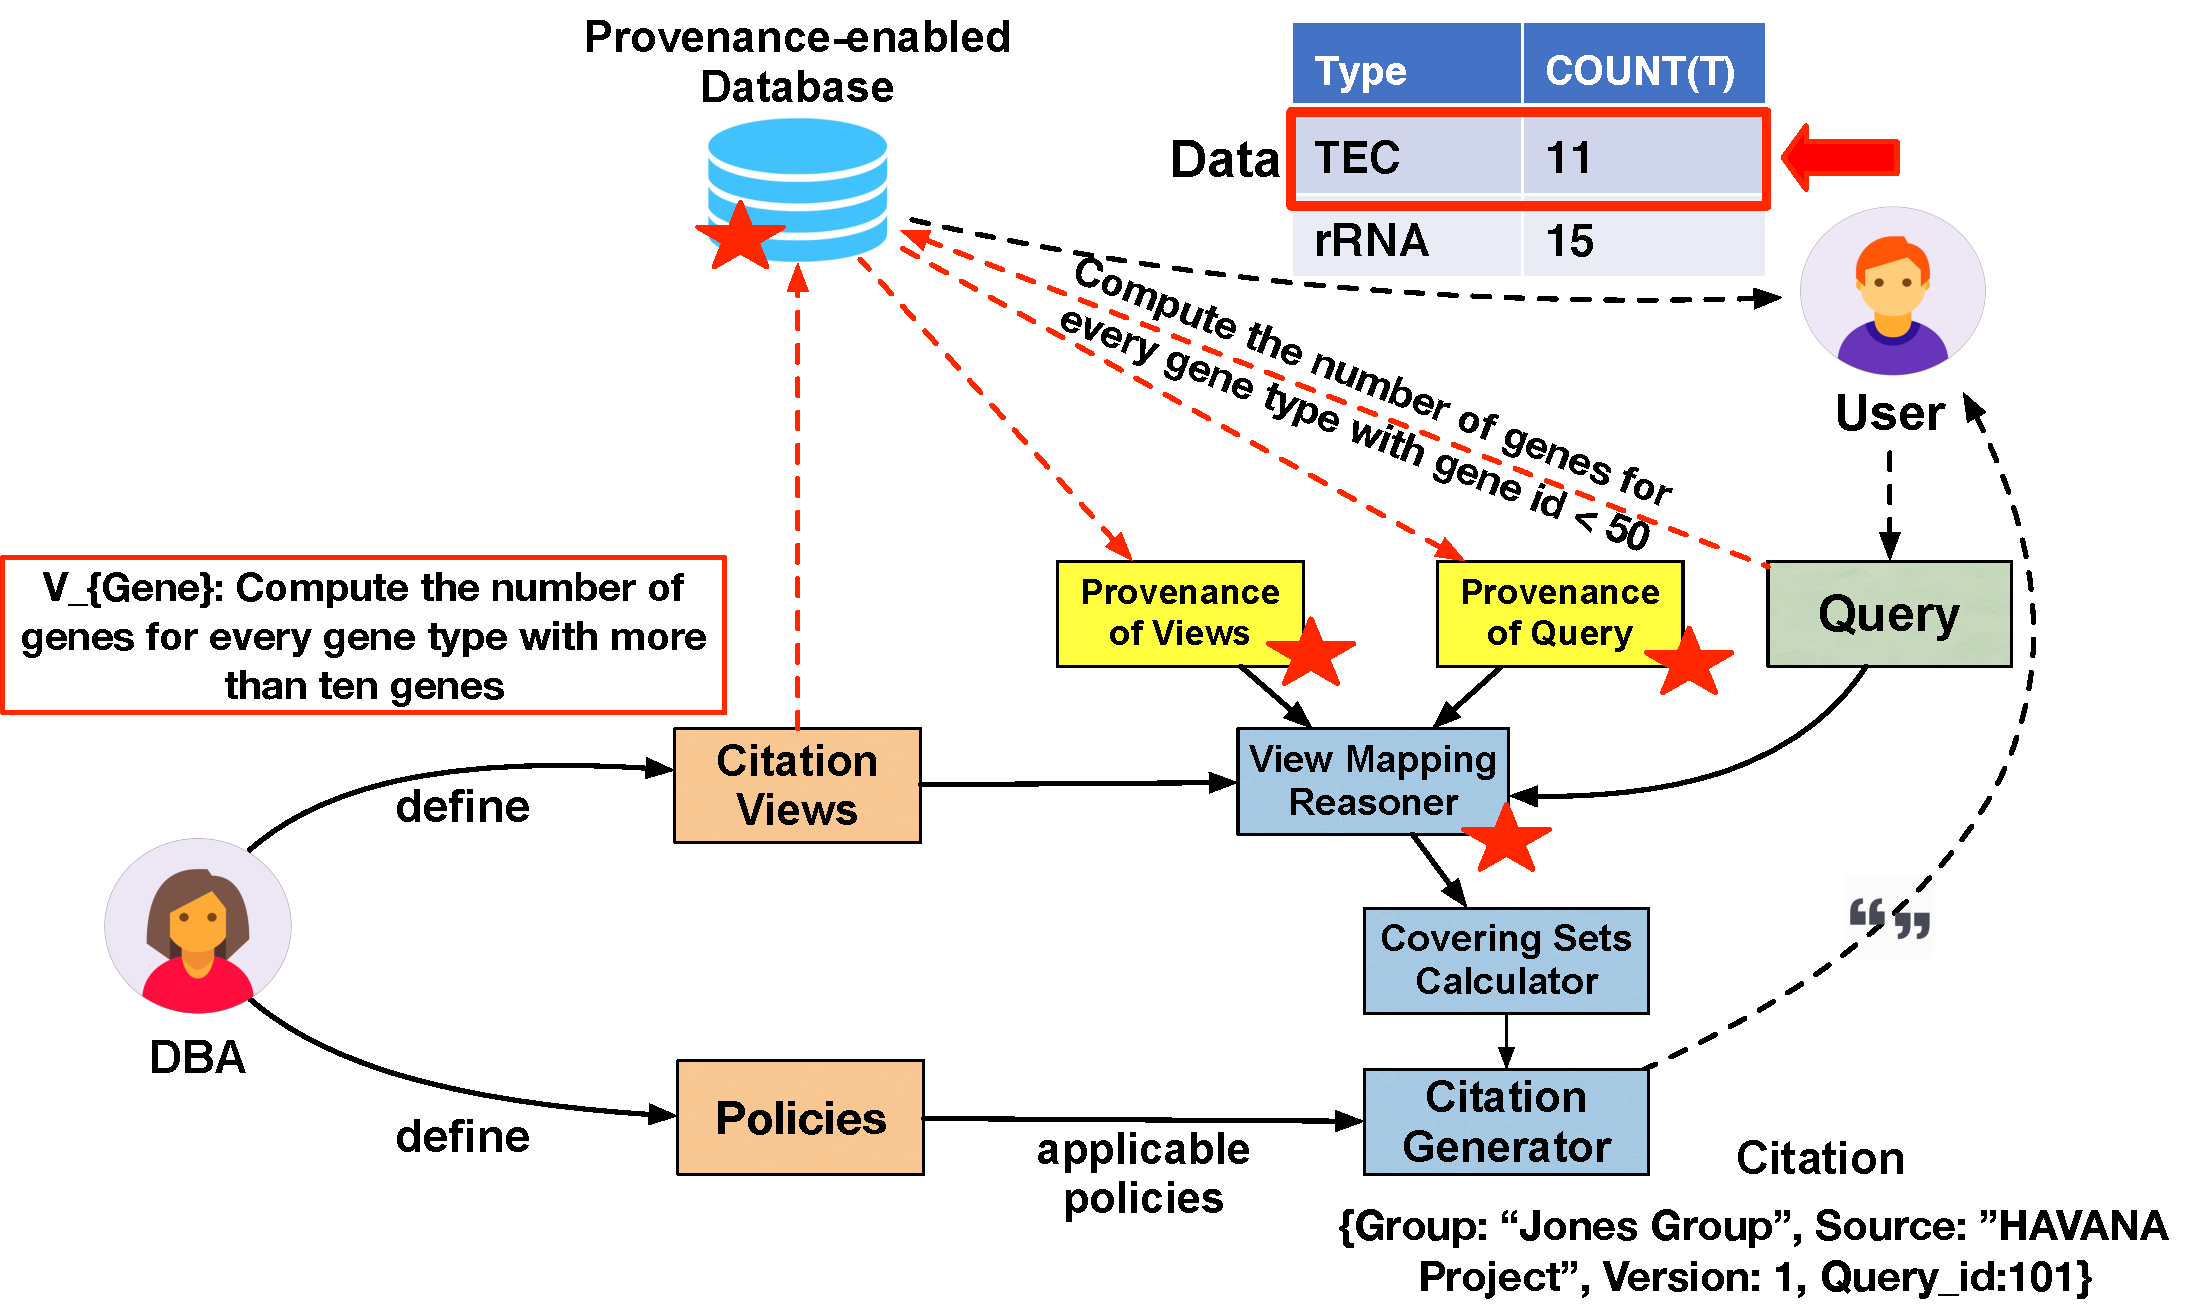
\includegraphics[width=0.48\textwidth,height=0.25\textwidth]{Figures/general_citaiton_framework.pdf}
%    \caption{System overview of ProvCite}
%    \small \label{fig:DataCitationFW}
%\end{figure}

%contributions
{\textbf{Contributions}} of this paper include:
\begin{enumerate}
\item A framework formalizing the connection between data provenance and data citation.

\item %\scream{claim general agg function is supported} 
A semantics for generating citations to the results of aggregate queries with {\em general aggregate functions} given a set of either aggregate or conjunctive views using provenance in the view and query instances. 

\item An implementation of \pba\ called ProvCite, which automatically generates fine-grained citations for the results of general queries, where both the queries and views may involve aggregates. The implementation includes multiple dedicated optimizations. 
%Some optimization strategies were used, which are also applicable in other scenarios wherever the provenance from different queries or views needs to be compared, such as fine-grained access control \cite{goyal2006attribute} and linked brushing in data visualization \cite{psallidas2018smoke}.

\eat{Two strategies are tested for the provenance of views: In the first, provenance is generated on the fly ({\em lazy strategy}), whereas in the second provenance is pre-computed ({\em eager strategy}).}
\item 
An experimental study using both {\em synthetic}  and {\em realistic} workloads, showing the efficiency of the approach and the effectiveness of the developed optimizations.

%comparing 
%\provalg\ against \rba\ approaches~\cite{wu2018data} in the case of aggregate queries and conjunctive views, and measuring the effect of the optimization strategies for \provalg\ when queries and views involve aggregates.  
\eat{ In {\em synthetic workloads}, the new approach is compared to prior approaches (TLA and SSLA) in the case where all views are $\mathcal{CV}$ while ({\em virtualization strategy}) and ({\em materialization strategy}) are compared to each other in the case where all views are $\mathcal{CAV}$ (which cannot be handled by TLA or SSLA).}
%The results show that \provalg\ has acceptable time performance even when the queries and views have large instances, and can in some cases significantly outperform \rba\ approaches.
\eat{feasible in time performance no matter whether the provenance of views are materialized or virtual even when queries and views have large instances; 2) compared to TLA and SSLA, the provenance approach is even about 2x faster than TLA and SSLA in some cases. }
\end{enumerate}

\eat{Yinjun, there are too many sections.  Perhaps fold background information into the model, and/or the algorithm?}
The rest of this paper is organized as follows.
Related work is discussed in Section~\ref{Sec: related_work}, and the running example and preliminaries are given in Section~\ref{Sec: examples}.  Details of the \pba\ and its implementation in ProvCite are presented in Sections~\ref{sec: model} and~\ref{Sec: implementation} respectively. Section~\ref{sec:experiments} gives experimental results before concluding in Section~\ref{sec: conclusion}.


% We have developed a model for automating data citation and implemented three approaches for generating citations at various levels of granularity (tuple level, semi-schema level, and schema level)~\cite{wu2018data}.  The model, however, only works for non-recursive conjunctive queries ($\mathcal{CQ}$) and non-recursive conjunctive views ($\mathcal{CV}$). In this work, we propose a model that uses {\em provenance} to support more complicated queries, i.e. non-recursive select-project-join-aggregate (SPJA) queries ($\mathcal{CAQ}$) and non-recursive select-project-join-aggregate (SPJA) views ($\mathcal{CAV}$). In both $\mathcal{CAQ}$ and $\mathcal{CAV}$, the aggregate operator can only occur as the last step in the query plan (no aggregation in sub-queries), and may have conditions over aggregates (i.e, the HAVING clause)

% In this section, we assume that the form of both the query and views is . 
% To represent such  queries, we use an extended version of Datalog called S-Datalog \cite{consens1990low}, an extension which is commonly used in work on query rewriting using views with aggregation \cite{cohen2006user}\cite{cohen2006rewriting}. In this section, the aggregate operator can only occur as the last step in the query plan (no nesting), and may have conditions over aggregates (i.e, the HAVING clause in SQL) in views and queries, which is not considered in \cite{cohen2006rewriting}.


% \subsection{Why aggregate queries and views}
% In several applications, we have found that users are interested in extracting \textit{summaries} from a database by issuing aggregate queries. 

% Although aggregate queries are common in Hetionet, the citable objects (view queries) are in $\mathcal{CV}$. In this case the reasoning is not very different from the conjunctive query case. 
% We therefore have another example, GENCODE\footnote{www.gencodegenes.org}, where \textit{both the queries and views} are $\mathcal{CAQ}$.  In this case, the reasoning becomes more interesting.

% Since neither of these examples are intuitive, in the paper (to be written) we will develop complex queries and views using a database of computer science publications (extracted from DBLP) and funding sources (extracted from the NSF website).  We will mention, but not build on, the use cases of Hetionet, IUPHAR and GENCODE.

\section{Related work}\label{Sec: related_work}

%from digital library domain
{\em Data citation.} Principles for data citation have been proposed within the digital libraries community\cite{CODATA2013,FORCE11_2104} 
%by CODATA~\cite{CODATA2013} and FORCE 11~\cite{FORCE11_2104}, 
and include: 1) identification and access to the cited data; 2) persistence of the cited data; and 3) completeness of the reference~\cite{Klump2015,Simons12,BraseSL15,DataCite2016}. 
The community also recognized the importance of citations to aggregate data~\cite{CODATA2013}, as have various scientific communities~\cite{harrow2012gencode, himmelstein2017systematic, mcentyre2015biostudies}. 
%, which couldn't be handled at the same time by previous efforts 
More recently, data citation has captured the attention of database researchers, who formulated computational challenges~\cite{BunemanEtAl2016, DBLP:conf/pods/DavidsonBDMS17}.
To address these challenges, a model of {\em citation views} was defined in \cite{davidson2017model} and implemented in \cite{alawini2017automating,wu2018data}.  However, this work was limited to conjunctive queries and views, and did not address aggregates. 
% constructing citations for {\em aggregated data} has become a major concern. Some principles for data citations have been come up with especially for aggregated data. For example, CODATA \cite{CODATA2013} proposes one such principle, i.e. {\em Citations should facilitate the establishment of provenance of aggregated data}.


%{\em Query rewriting using views with aggregation} 
{\em Query rewriting using views.} %As \cite{wu2018data} claimed, 
Data citation is closely related to the problem of query rewriting using views.
%, which reasons about how to use a set of views $\mathcal{V}$ to ``rewrite'' a given query $Q$.  
Rewriting relies on notions of {\em containment} and {\em equivalence} of queries \cite{halevy2001answering}, and has been extensively studied 
in the context of conjunctive queries \cite{chandra1977optimal, chaudhuri1995optimizing, pottinger2000scalable, afrati2007using} as well as aggregate queries~\cite{cohen2007deciding, cohen1999rewriting}. 
% Unlike conjunctive queries, for which containment and equivalence use a {\em set semantics}, aggregate queries use a {\em bag-set semantics} for containment and equivalence.
%is applied to determine the containment and equivalence between queries, which takes the operands of queries (query result) as set (bag).
Various algorithms have been designed to rewrite aggregate queries.
% using the {\em bag-set semantics}. 
For example, \cite{srivastava1996answering, galindo2001orthogonal} provide algorithms for determining whether a materialized view is usable for answering an aggregate query by considering both conjunctive and aggregate views.
In \cite{zaharioudakis2000answering}, an algorithm is given to handle nested subqueries and multidimensional aggregations in queries and views. However, only standard aggregate functions (e.g. SUM, COUNT) are considered in ~\cite{zaharioudakis2000answering, srivastava1996answering, galindo2001orthogonal}; general aggregate functions (such as
user defined aggregate functions) cannot be used. The problem of general aggregate functions is considered in \cite{cohen2006rewriting}, and \cite{cohen2006user} bridges the gap between theory and practice by providing  implementation suggestions. However, to our knowledge, there is no work which considers how to rewrite queries using \textit{general aggregate views with having clauses}.

{\em Data Provenance.} Data provenance identifies where a piece of data came from and the process by which it arrived in the database \cite{buneman2001and}.  It has been used to track the dependencies between inputs and outputs, detect errors in complex workloads, and provide explanations for debugging purposes. Various formulations of provenance have been studied, such as \textit{why- and where-provenance} \cite{buneman2001and}, \textit{why-not-provenance} \cite{chapman2009not}, and the \textit{provenance semirings} framework %(how-provenance) 
for conjunctive queries \cite{green2007provenance}, aggregate queries \cite{amsterdamer2011provenance} and queries with negation \cite{xu2018provenance}.  This framework has been used to implement several practical provenance-enabled database systems, such as ORCHESTRA \cite{ives2008orchestra} and GProM \cite{arab2018gprom}. The connection between data citation and provenance was discussed in \cite{BunemanEtAl2016} and explored but not formalized in \cite{alawini2018data}. This paper develops those ideas further, provides an implementation based on a provenance-enabled database system, and shows the feasibility of the approach.


\section{Preliminaries}\label{Sec: examples}
In this section, we introduce the running example, %, a simplification of GENCODE, 
review the notions of \textit{citation views}~\cite{davidson2017model}, {\em view mapping} and {\em validity} of view mappings \cite{wu2018data}, and then show why the \rba\ of \cite{wu2018data} cannot be extended for aggregate queries and views, motivating the need for {\em provenance}.
% discuss why query rewriting using views is not enough for fine-grained citation, and show why the approach in~\cite{wu2018data} works for fine-grained citation in \textit{conjunctive} queries and views but not for \textit{aggregate} queries and views.

\subsection{Running example: GENCODE}\label{subsec:running example}

\eat{\begin{figure}[t!]
    \centering
    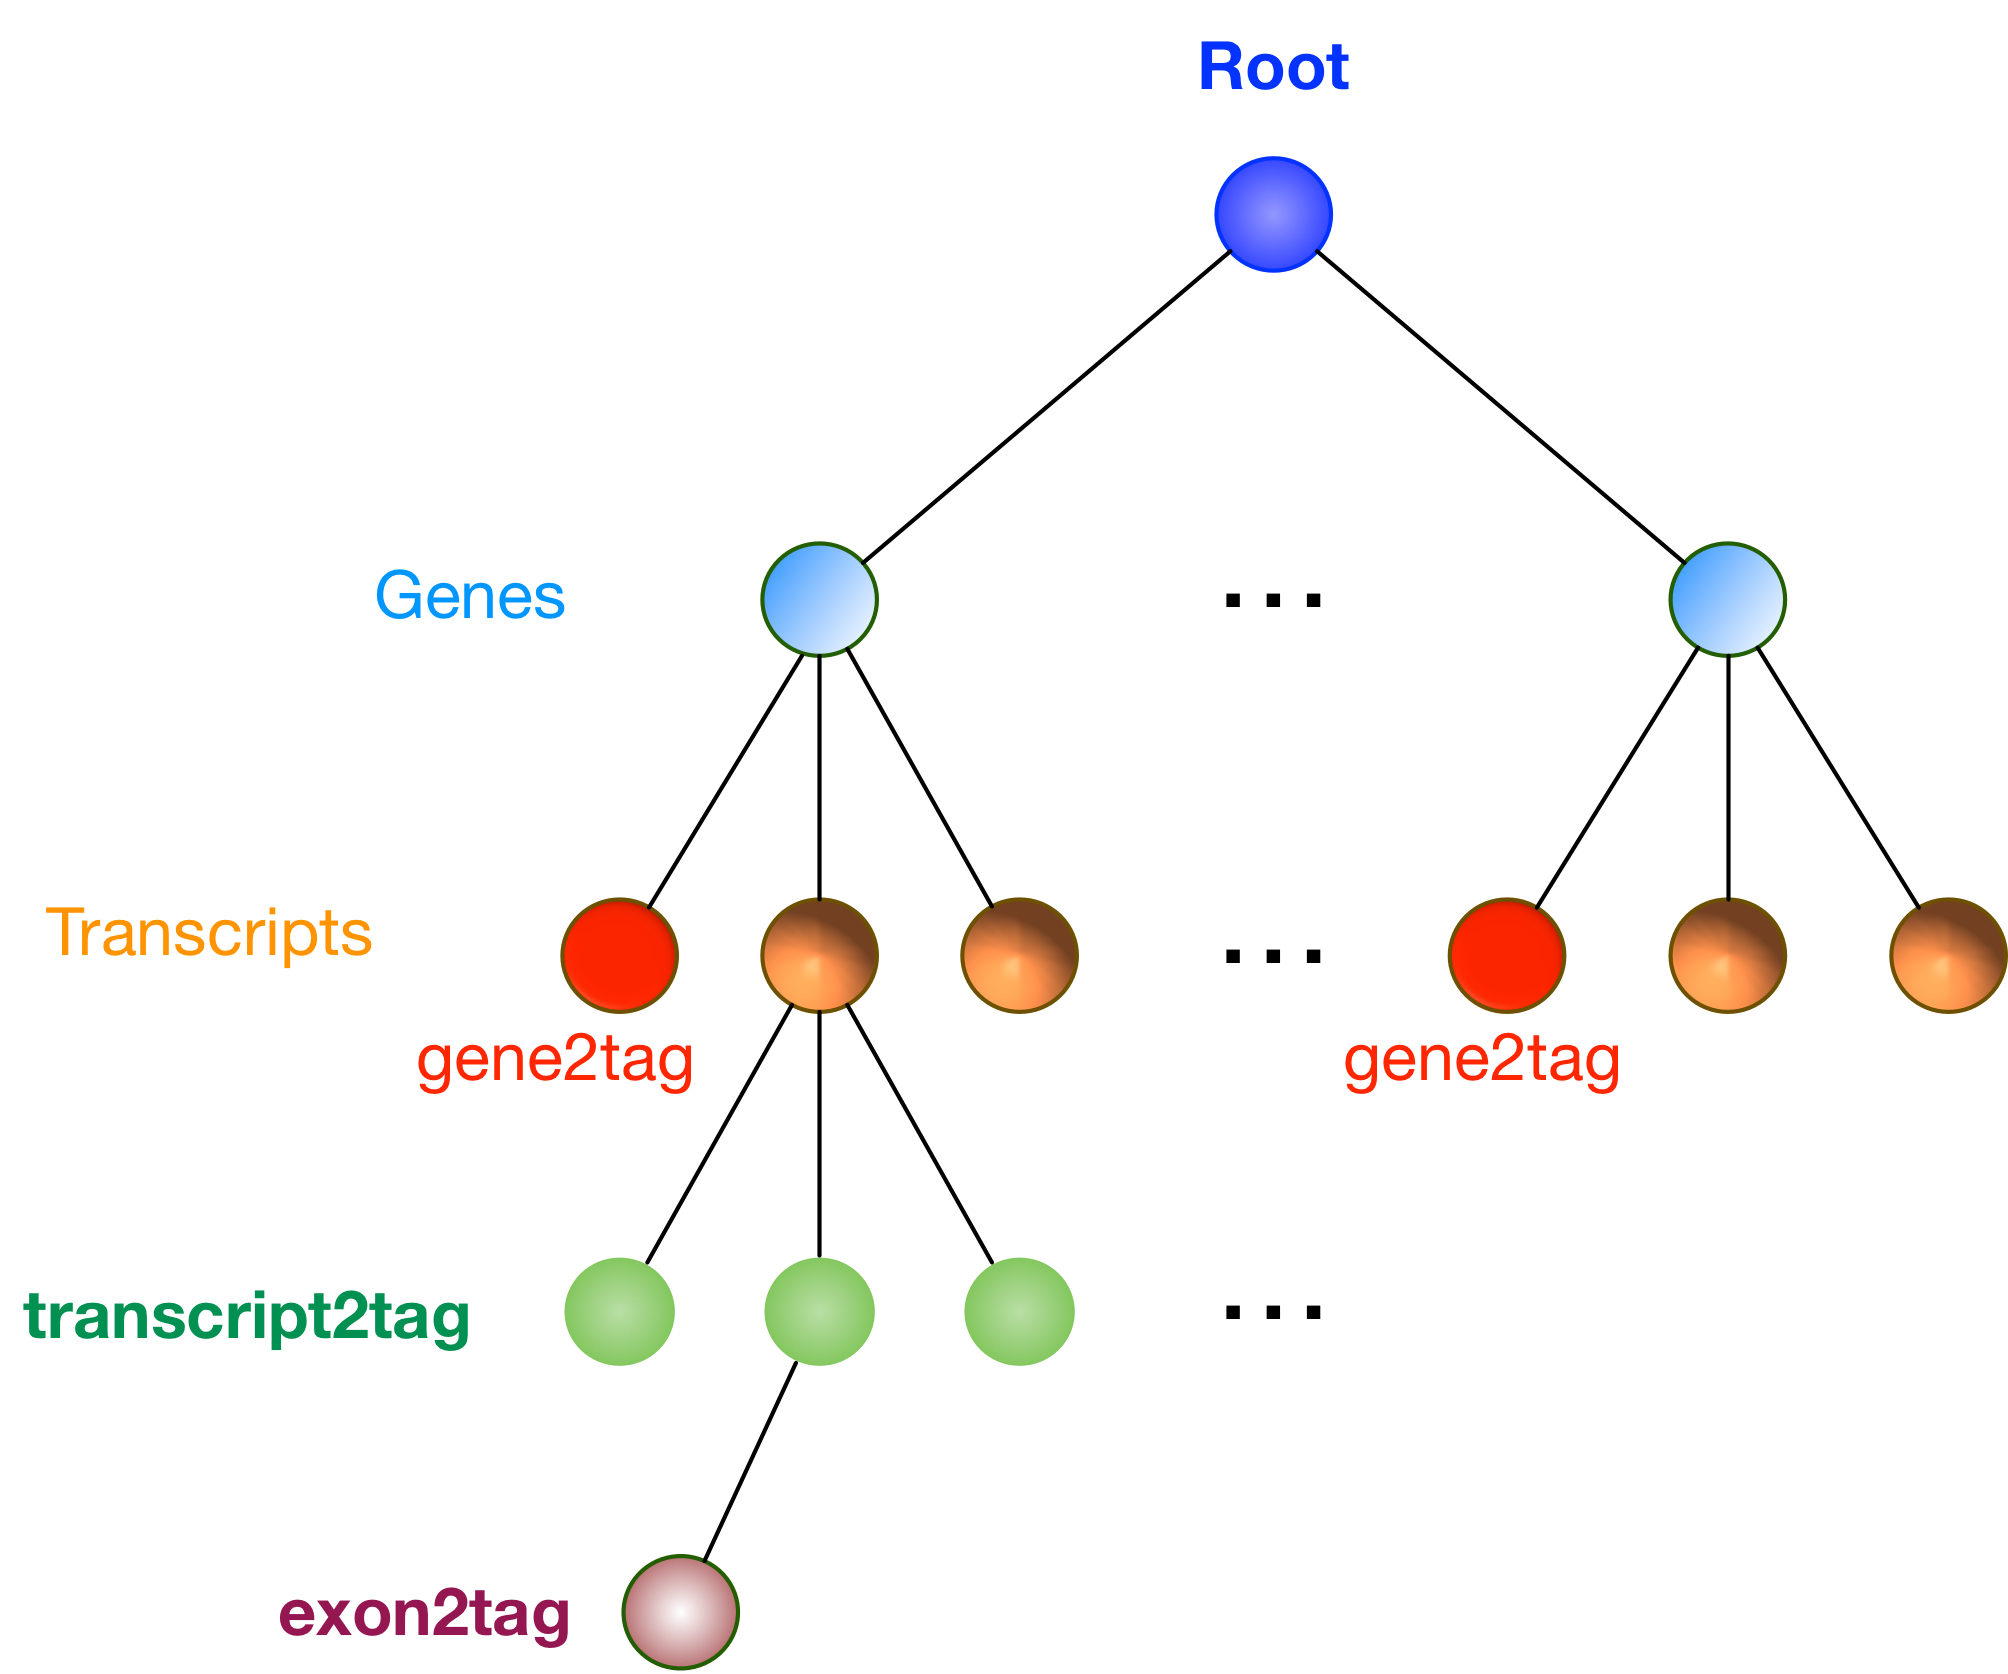
\includegraphics[width=0.4\textwidth,height=0.24\textwidth]{Figures/Gens_Trans_Tree.jpg}
    \caption{Hierarchical structure in GENCODE}
    \small \label{fig:gencode}
\end{figure}}


We use a simplified schema from GENCODE as our running example. In this database, information is structured hierarchically\eat{ (see Figure \ref{fig:gencode})}: Each gene is associated with one or more transcripts, and each transcript has one or more exons. Genes, transcripts, and exons may all be annotated with tags, which are created either by human experts or by programs. A simplified schema based on this structure is shown below:

\begin{tabbing}
%\begin{tabular}{l}
Gene(\underline{GID}, Name, Type)\\
Gene2tag(GID, annot) GID references Gene\\
Transcript(\underline{TID}, Name, Type, GID) GID references Gene\\
Transcript2tag(TID, annot) TID references Transcript\\
Exon(\underline{EID}, Level, TID), TID references Transcript\\
Exon2tag(EID, annot), EID references Exon
% \hspace{0.85in} PID references Person\\
% Person(\underline{PID}, PName, Affiliation)\\
% Gene2P(\underline{GID}, \underline{PID}), GID references Gene, PID references Person\\
% Transcript2P(\underline{TID}, \underline{PID}), TID references Transcript, 
% \\PID references Person\\
% Exon2P(\underline{EID}, \underline{PID}), EID references Exon, PID references Person\\
% \hspace{0.85in}  \\
% MetaData(Type, Value)\\
%\end{tabular}
\end{tabbing}
Relations Gene2tag, Transcript2tag and Exon2tag capture the annotations ({\em annot}). 
% For example, some genes were given annotation ``overlapping locus'', which indicates that ``exon(s) of the locus overlap exon(s) of a readthrough transcript or a transcript belonging to another locus''\footnote{http://vega.archive.ensembl.org/info/about/annotation\_attributes.html}. 
The source of the annotation (e.g. a research group or workflow/program) is also stored in GENCODE and can be used for citations.  For simplicity, we omit these relations.
\eat{
research groups involved in Havana project\footnote{https://www.sanger.ac.uk/science/groups}), which implies citations. Such citation information is also stored in GENECODE and ready for generating formated citations when the corresponding data are cited.}

\textit{Citation views}~\cite{davidson2017model} define views of the database to which citations have been specified.  A citation view consists of 1) a \textit{view query}, defining the subset of the data to which the citation is attached; 2) a \textit{citation query}, which retrieves information required for the citation for the view; and 3) a \textit{citation function}, which formats the information retrieved by the citation query to provide the final citation, e.g. in JSON, BibTex or RIS format. View queries can be considered to be the \textit{frequent queries} over the database; all other queries will be called \textit{general} queries.
\eat{
Since the reasoning involved in generating a citation to a general query involves reasoning over the view queries, we focus on view queries.}

View queries for GENCODE correspond to web-page views  created by the DBAs.  Each of these views could have an associated citation.  For example, the citation query for the web page view of a gene could be used to retrieve the research groups or programs that contributed annotations for the gene; this information, together with the gene name, version of the database, and query used to retrieve the data (e.g. the http address of the web page) could then be formatted by the citation function.
\eat{
For on-line scientific databases like GENCODE, the citation views are defined by DBAs and used to represent the on-line webpages (i.e. cited data) associated with hard-coded citations. For example, for the simplified schema, to mimic those existing citations on line, the {\em view definitions} could be:} 
Below we show several of these views, which are expressed using S-Datalog \cite{consens1990low}, an extended version of Datalog that allows aggregates:
\noindent
\begin{tabbing}
$\lambda G.$\=$V_1(G, Ty) $\hspace{6em}\=$:-$\=$ Gene(G, N, Ty), G \leq 2$\\
\> $V_2(Ty, COUNT(G)) $\>$:-$\>$ Gene(G, N, Ty), Ty = `rRNA$'\\
% \>\>\>$ Exon(E, L, T2), T1=T2$\\
\> $V_3(T1, E, G1, L)$\>$:-$\>$Transcript(T1, N1, Ty1, G1),$\\
% \>\>\>$Gene(G1, N1, Ty1), G1 = G2,$\\
\>\>\>$Exon(E, L, T2), T1 = T2,$\\
\>\>\>$E \leq 2$\\
\> $V_4(G1, COUNT(T1))$\>$:-$\>$Transcript(T1, N1, Ty1, G1),$\\
\>\>\>$Exon(E, L, T2), T1 = T2, $\\
\>\>\>$L \leq 2$\\
\>$V_5(G1, MAX(L), COUNT(E))$\\
\>\>$:-$\>$Transcript(T1, N1, Ty1, G1),$\\
\>\>\>$Exon(E, L, T2), T1 = T2$\\
\> $V_6(G, COUNT(T)) $\>$:-$\>$ Transcript(T, N, Ty, G)$
\end{tabbing}
$V_1$ and $V_3$ are simple conjunctive queries. % and %belong to $\mathcal{CV}$ 
%are simple conjunctive queries.  
$V_1$ is \textit{parameterized} by the gene id $G$, meaning that it defines a family of views, one for each gene. Each view in this family consists of a single tuple.  In this way, each gene may have different citation, giving credit to the person or program who annotated that gene. 
In contrast, $V_3$ is not parameterized, which indicates that the same citation is shared across all the view tuples.\eat{Maybe we don not need the figure, just point to SIGMOD paper}
% Figure \ref{fig:lambda} shows the effect of the lambda term in $V_1$ versus the unparameterized view $V_2$ on a sample instance of Gene.
% is parameterized by the transcript id $T$,
%and includes the id ($T$), name ($N$) and type ($Ty$) of the transcript, 
% enabling each transcript to have a different citation. 
% The view for each gene and transcript includes information about the 
\eat{\begin{figure}[t!]
    \centering
    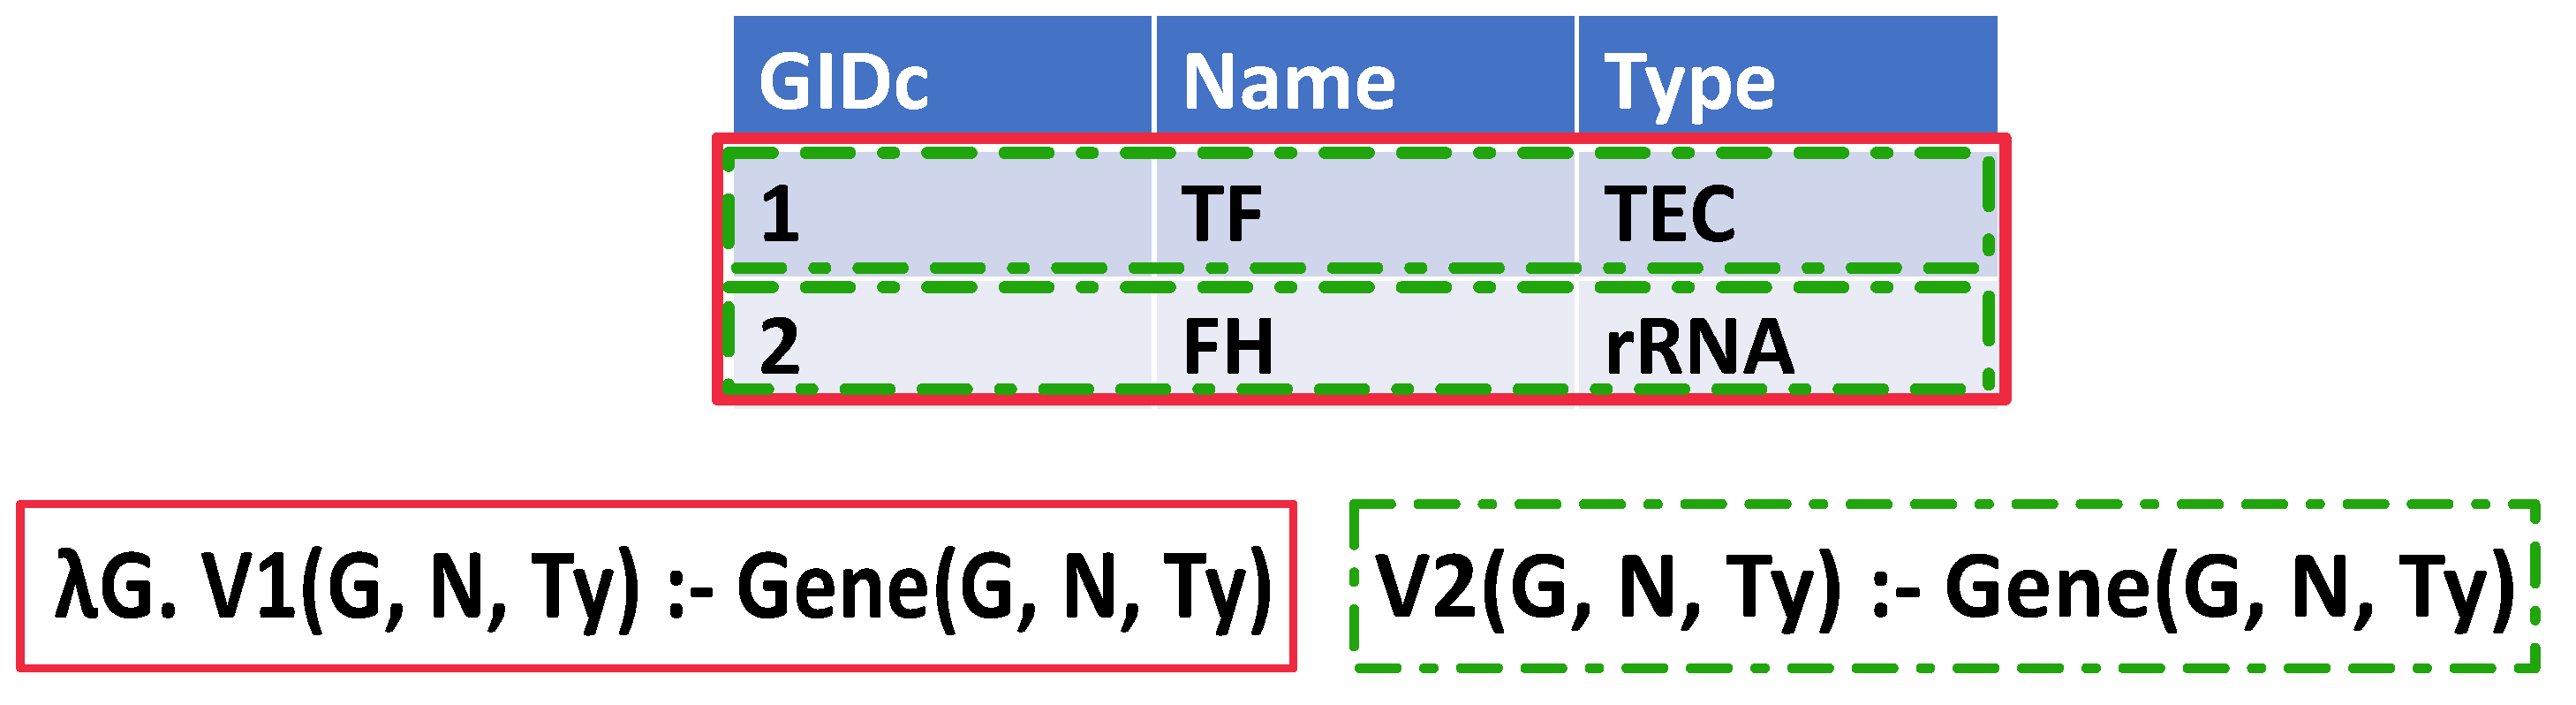
\includegraphics[width=0.45\textwidth,height=0.11\textwidth]{Figures/GIDsExample.pdf}
    \caption{Effect of parameters on views}
    \small \label{fig:lambda}
\end{figure}}
The other four views are aggregate views. Their meaning is: for each binding of variables in the body, group over the variables  in the head (called {\em grouping variables}) and apply the aggregate(s) to each group. Each {aggregate function} along with its arguments is called an {\em aggregate term}, in which the arguments are called {\em aggregate variables}.
Thus $V_2$ could be translated into SQL as:
\begin{tabbing}
SELECT G.Type, COUNT(G.GID)\\
FROM Gene G\\
WHERE G.Type = `rRNA'\\
GROUP BY G.Type
\end{tabbing}
% \begin{tabbing}
% SELECT T.GID, COUNT(T.TID)\\
% FROM Transcript T, Exon E\\
% WHERE T.TID=E.TID and E.Level $\leq$ 2\\
% GROUP BY T.GID
% \end{tabbing}
which counts the number of `rRNA' genes. Similarly, $V_4$ counts the number of transcript associated with one exon whose level is not greater than 2 for each gene.
$V_5$ returns the maximal level of exons and the count of exons for each gene.
$V6$ counts the number of transcripts for each gene.

\subsection{Query rewriting:  View mappings}
%\scream{I think we need to cover more concepts here, e.g. the notion of mapping and covering}
Given a (general) query $Q$ and a set of views $\mathcal{V}$, the \rba\ implementation in~\cite{wu2018data} starts by building a set of \textit{view mappings} $\mathcal{M}$ from $\mathcal{V}$ to $Q$. For each query tuple, \rba\ then reasons about the {\em validity} of each view mapping in $\mathcal{M}$ and constructs {\em covering sets}, which are converted to formatted citations later. Each covering set is a \textit{maximal}, \textit{non-redundant} set of {\em valid} view mappings,
% Since there may be many such covering sets, only \textit{maximal}, \textit{non-redundant} covering sets are considered, 
i.e. covering sets for which no other view mappings can be added to \textit{cover} more subgoals and head variables in $Q$, nor can any be removed and still \textit{cover} the same subgoals and head variables in $Q$.

%According to \cite{wu2018data}, a
\eat{here}
A \textit{view mapping} $M$ consists of a {\em relation mapping}, $h$ and {\em variable mapping}, $\phi$ (denoted $M=(h, \phi)$). The former, $h$, maps relational subgoals in a view $V$ to relational subgoals with the same relation names in query $Q$, while the latter variable mapping $\phi$ is an induced mapping by $h$. 
% We say that a head variable of $Q$, $x$ is {\em covered} under $M$ iff there exists a head variable $y$ of $V$ such that $\phi(y) = x$.

Intuitively, for a query tuple $t$, view mapping $M$ is valid iff there exists a view tuple $t'$ in $V$ such that $t'$ is {\em visible} in $t$ under $M$, the reasoning of which depends on examining the lambda variables, the head variables and predicates of views by \rba\ in \cite{wu2018data}. We say that a head variable or a relational subgoal of $Q$ is {\em covered} by $M$ iff it is involved in $M$.

\eat{In the remainder of this paper, we will call the model in \cite{wu2018data} 
the \textit{Rewriting-based Model}.} \eat{maybe we don't need it since we call the approach RBA}

\eat{Need to call this "V\_6" or something... I don't understand the numberings.}

\begin{example}\label{eg: conjunctive_case}
Suppose a conjunctive query is defined below:
\begin{tabbing}
$Q_{\ref{eg: conjunctive_case}}(T, Gid) $\hspace{0.05em}$:- Gene(Gid, Name, T), Gid \leq 3$
\end{tabbing}
There is a view mapping $M_{1\ref{eg: conjunctive_case}} = (h_{1\ref{eg: conjunctive_case}}, \phi_{1\ref{eg: conjunctive_case}})$ from $V_1$ to $Q_{\ref{eg: conjunctive_case}}$, in which the relation mapping $h_{1\ref{eg: conjunctive_case}}$ is $\{Gene(G, N, Ty) \rightarrow Gene(Gid, Name, T)\}$ while the variable mapping $\phi_{1\ref{eg: conjunctive_case}}$ is $\{G\rightarrow Gid, N \rightarrow Name, Ty\rightarrow T\}$. $M_{1\ref{eg: conjunctive_case}}$ is only valid for query tuples with $Gid \leq 2$ since 1) those query tuples can appear in the instance of $V_1$ by satisfying predicate $G \leq 2$; and 2) the head variables $G$ (also lambda variable) and $Ty$ in $V_1$ are mapped to head variables $Gid, T$ in $Q_{\ref{eg: conjunctive_case}}$ respectively, which implies {\em visibility}. \rba\ determines the validity by checking whether the portion of a query tuple $t$ ``exists'' under the view mapping in the view instance, which is achieved by evaluating the predicates in the views along with the executions of the query. So $Q_{\ref{eg: conjunctive_case}}$ is rewritten as:


\begin{tabbing}
$Q_{\ref{eg: conjunctive_case}}(T, Gid,(Gid \leq 2))$\hspace{0.1em}\=$:-Gene(Gid, Name, T),Gid <= 3$
\end{tabbing}

The instance of $Q_{\ref{eg: conjunctive_case}}$ is shown in Table \ref{Table: Instance of Q1} (ignore the last column temporarily), in which the boolean expression $(Gid \leq 2)$ (derived from the predicate of $V_1$) is also evaluated. The truth or false value indicates the {\em existence} or {\em non-existence} of the query tuple in the view instance under the view mapping. For instance, $t_{q_{\ref{eg: conjunctive_case}}1}$ makes all the predicates in $V_1$, i.e. $(Gid \leq 2)$ true since $t_{q_{\ref{eg: conjunctive_case}}1}$ ``exists'' in the instance of $V_1(D)$ (i.e. $t_{v_11}$, under the mapping $M_{1\ref{eg: conjunctive_case}}$) while the false value in $t_{q_{\ref{eg: conjunctive_case}}3}$ is due to the fact that it is missing from $V_1(D)$.
% its satisfiability for each $(T, Gid)$ pair. Under a view mapping $M$ (e.g. $M_{1\ref{eg: conjunctive_case}'}$), only if all the corresponding view predicates (e.g. $(Gid \leq 2)$ for $M_{1\ref{eg: conjunctive_case}'}$) are satisfied for a query tuple $t$, $M$ is determined as a valid view mapping for $t$.

For the query tuples for which $M_{1\ref{eg: conjunctive_case}}$ is a valid view mapping, one covering set can be constructed:  \{$M_{1\ref{eg: conjunctive_case}}$\}. After the user selects the query subset or the entire query result,  the \textit{citation queries} associated with $V_1$ are executed and the {\em citation function} is applied to construct formatted citations.
\end{example}
\eat{
\begin{example}\label{eg: conjunctive_case}
Suppose a conjunctive view and a conjunctive query are defined below:
\begin{tabbing}
$V_{\ref{eg: conjunctive_case}}'(E, T)$\hspace{0.05em}\=$:-$\=$ Exon(E, L, T), E <= 4$\\
%$Q_{\ref{eg: illustrative_eg3}}(Tid, AVG(Level)) $\>$:-$\>$ Exon(Eid, Level, Tid), Tid = 2$
$Q_{\ref{eg: conjunctive_case}}'(Eid, Tid) $\hspace{0.05em}$:- Exon(Eid, Level, Tid)$
\end{tabbing}
There is a view mapping $M_{\ref{eg: conjunctive_case}}' = (h_{\ref{eg: conjunctive_case}}', \phi_{\ref{eg: conjunctive_case}}')$ from $V_{\ref{eg: conjunctive_case}}'$ to $Q_{\ref{eg: conjunctive_case}}'$, in which the relation mapping $h_{\ref{eg: conjunctive_case}}'$ is $\{Exon(E, L, T) \rightarrow Exon$ $(Eid, Level, Tid)\}$ while the variable mapping $\phi_{\ref{eg: conjunctive_case}}'$ is $\{E\rightarrow Eid, L \rightarrow Level, T\rightarrow Tid\}$. $M_{\ref{eg: conjunctive_case}}'$ is only valid for query tuples with $Eid <= 4$ since 1) all the view tuples in $V_{\ref{eg: conjunctive_case}}'$ satisfy $E <= 4$; and 2) no lambda variables in $V_{\ref{eg: conjunctive_case}}'$ and the head variables $E, T$ in $V_{\ref{eg: conjunctive_case}}'$ are mapped to head variables $Eid, Tid$ in $Q_{\ref{eg: conjunctive_case}}'$ respectively, which implies {\em visibility}. For the query tuples for which $M_{\ref{eg: conjunctive_case}}'$ is a valid view mapping, one covering set can be constructed:  \{$M_{\ref{eg: conjunctive_case}}'$\}. After the user selects the query subset or the entire query result,  the \textit{citation queries} associated with $V_{\ref{eg: conjunctive_case}}'$ are executed and the {\em citation function} is applied to construct formatted citations.
\end{example}}

% rewriting \textit{each tuple $t$ in the result of} $Q$ in terms of $\mathcal{V}$ (fine-grained citations).  

% Each rewriting involves a subset of the views, whose citations are {\em jointly used} (*) to construct a possible citation for $t$.  Since there may be multiple rewritings for $t$, the citations of each rewriting are {\em alternatively used} (+) to construct the citation for $t$.  Reasoning is done at the level of the schema of views. 



\subsection{The need for provenance}
\label{ssec:need-provenance}


\begin{table}[htp]
\centering
\small
% \caption{Sample instance of relation $Transcript$ with how- and where-provenance}\label{Table: Sample instance of Transcript}
% \begin{tabular}[t]{c|c|c|c|c|c|c|c|c|c|} \hhline{~---------}
% &TID&&Name&&Type&&GID&&\\ \hhline{~---------}
% $t_{1}$&1&$a_1$&TF&$b_1$&TEC&$c_1$&1&$d_1$&$T_1$\\ \hhline{~---------}
% $t_{2}$&2&$a_2$&FH&$b_2$&rRNA&$c_2$&1&$d_2$&$T_2$\\ \hhline{~---------}
% $t_{3}$&3&$a_3$&HP&$b_3$&rRNA&$c_3$&1&$d_3$&$T_3$\\ \hhline{~---------}
% $t_{4}$&4&$a_4$&GK&$b_4$&TEC&$c_4$&2&$d_4$&$T_4$\\ \hhline{~---------}
% $t_{5}$&5&$a_5$&F7&$b_5$&rRNA&$c_5$&1&$d_5$&$T_5$\\ \hhline{~---------}
% \end{tabular}
\caption{Instance of relation $Exon$ with provenance}\label{Instance of Exon}
\begin{tabular}[t]{c|c|c|c||b|} \hhline{~----}
&EID&Level&TID&prov\\ \hhline{~----}
$t_{e1}$&1&1&1&$e_1$\\ \hhline{~----}
$t_{e2}$&2&3&2&$e_2$\\ \hhline{~----}
$t_{e3}$&3&3&2&$e_3$\\ \hhline{~----}
$t_{e4}$&4&2&4&$e_4$\\ \hhline{~----}
$t_{e5}$&5&3&5&$e_5$\\ \hhline{~----}
$t_{e6}$&6&2&5&$e_6$\\ \hhline{~----}
$t_{e7}$&7&2&5&$e_7$\\ \hhline{~----}
\end{tabular}
\bigskip
\caption{Instance of relation $Gene$ with provenance}\label{Instance of Gene}
\begin{tabular}[t]{c|c|c|c||b|} \hhline{~----}
&GID&Name&Type&prov\\ \hhline{~----}
$t_{g1}$&1&TF&TEC&$g_1$\\ \hhline{~----}
$t_{g2}$&2&FH&rRNA&$g_2$\\ \hhline{~----}
$t_{g3}$&3&RP1&rRNA&$g_3$\\ \hhline{~----}
$t_{g4}$&4&IYD&rRNA&$g_4$\\ \hhline{~----}
$t_{g5}$&5&EPN&mRNA&$g_5$\\ \hhline{~----}
\end{tabular}
\bigskip
\caption{Instance of relation $Transcript$ with provenance}\label{Instance of Transcript}
\begin{tabular}[t]{c|c|c|c|c||b|} \hhline{~-----}
&TID&Name&Type&GID&prov\\ \hhline{~-----}
$t_{t1}$&1&MB-203&TEC&1&$r_1$\\ \hhline{~-----}
$t_{t2}$&2&PC-203&rRNA&2&$r_2$\\ \hhline{~-----}
$t_{t3}$&4&HP-218&rRNA&3&$r_3$\\ \hhline{~-----}
$t_{t4}$&5&GK-207&rRNA&3&$r_4$\\ \hhline{~-----}
\end{tabular}
\end{table}



We now show how to reason about the {\em validity} of view mappings for query tuples in the context of aggregate queries and  views via an example, and illustrate how \rba\ can be extended for conjunctive views and why \rba\ fails for aggregate views, motivating the need for {\em provenance}.
% illustrate how aggregate queries can be rewritten in terms of aggregate views, and discuss why the approach is limited in some cases for reasoning about fine-grained citations, necessitating the use of provenance.




\eat{\begin{example}\label{eg: illustrative_eg1}
Suppose we have the following view ($V_{\ref{eg: illustrative_eg1}}$) and query  ($Q_{\ref{eg: illustrative_eg1}}$) defined over relation Transcript:
\eat{\begin{tabbing}
$V_{\ref{eg: illustrative_eg1}}(Ty1, G1, TOP2(T1))$\hspace{0.05em}\=$:-$\=$ Transcript(T1, N1, Ty1, G1)$\\
$Q_{\ref{eg: illustrative_eg1}}(Ty, MAX(T)) $\>$:-$\>$ Transcript(T, N, Ty, G), T <= 3$
\end{tabbing}}
\begin{tabbing}
$V_{\ref{eg: illustrative_eg1}}(T, COUNT(L), SUM(L))$\hspace{0.05em}\=$:-$\=$ Exon(E, L, T)$\\
%$Q_{\ref{eg: illustrative_eg1}}(AVG(Level)) $\>$:-$\>$ Exon(Eid, Level, Tid), Tid <= 3$
$Q_{\ref{eg: illustrative_eg1}}(AVG(Level)) $\hspace{0.05em}$ :- Exon(Eid, Level, Tid), Tid <= 3$
\end{tabbing}


\eat{$V_{\ref{eg: illustrative_eg1}}$ returns the top-2 transcript ids~\footnote{Note that this is not a 1NF result.} for each (gene,type),
whereas $Q_{\ref{eg: illustrative_eg1}}$ returns the largest transcript id for each (type).
It is easy to see that $V_{\ref{eg: illustrative_eg1}}$ can be used to rewrite $Q_{\ref{eg: illustrative_eg1}}$ by further aggregating $V_{\ref{eg: illustrative_eg1}}$ over $Ty$. The reason is as follows: First, there is a {\em view mapping} $M(h, \phi)$ from $V_{\ref{eg: illustrative_eg1}}$ to $Q_{\ref{eg: illustrative_eg1}}$, 
%which is composed of relational subgoal mapping $h$ and variable mapping $\phi$ (See details in \cite{wu2018data}). 
where $h$ maps relational subgoals of $V_{\ref{eg: illustrative_eg1}}$ to relational subgoals of $Q_{\ref{eg: illustrative_eg1}}$ with the same names (i.e. $\{Transcript \rightarrow Transcript\}$) and $\phi$ is an induced variable mapping of $h$ (i.e. $\{T1 \rightarrow T, N1 \rightarrow N, Ty1 \rightarrow Ty, G1 \rightarrow G\}$)~\cite{wu2018data}. Second, under $M$,  $V_{\ref{eg: illustrative_eg1}}$ \textit{does not project out any necessary columns and rows} for computing the query instance; this is done by comparing the head and predicates between the query and view~\cite{srivastava1996answering}. 
Third, there exists a {\em computation rule} from $TOP2$ to $MAX$, which indicates that for the same input, the output of $MAX$ function can be computed using the output of $TOP2$ function~\cite{cohen2006user}. We can therefore say that view mapping $M$ is a valid view mapping at the {\em schema level} for $Q_{\ref{eg: illustrative_eg1}}$~\cite{wu2018data}.}

$V_{\ref{eg: illustrative_eg1}}$ returns the number of exon levels ($COUNT(L)$) and the sum of exon levels ($SUM(L)$) for each Transcript id,
whereas $Q_{\ref{eg: illustrative_eg1}}$ returns the average level for all exons whose corresponding Transcript id is no more than 3.
It is easy to see that $V_{\ref{eg: illustrative_eg1}}$ can be used to rewrite $Q_{\ref{eg: illustrative_eg1}}$ by further aggregating $V_{\ref{eg: illustrative_eg1}}$ over $T$. More formally, this is because:  1) there is a {\em view mapping} $M=(h, \phi)$ from $V_{\ref{eg: illustrative_eg1}}$ to $Q_{\ref{eg: illustrative_eg1}}$, 
%which is composed of relational subgoal mapping $h$ and variable mapping $\phi$ (See details in \cite{wu2018data}). 
where $h$ maps relational subgoals of $V_{\ref{eg: illustrative_eg1}}$ to relational subgoals of $Q_{\ref{eg: illustrative_eg1}}$ with the same names (i.e. $\{Exon \rightarrow Exon\}$) and $\phi$ is an induced variable mapping of $h$ (i.e. $\{E \rightarrow Eid, L \rightarrow Level, T \rightarrow Tid\}$)~\cite{wu2018data}; 2) under $M$,  $V_{\ref{eg: illustrative_eg1}}$ \textit{does not project out any necessary columns and rows} for computing the query instance -- this is checked by comparing the head and predicates between the query and view~\cite{srivastava1996answering}; 
and 3) there exists a {\em computation rule} from $COUNT$ and $SUM$ to $AVG$, which indicates that for the same input, the output of $AVG$ function can be computed using the output of $COUNT$ and $SUM$ function~\cite{cohen2006user}. We can therefore say that view mapping $M$ is a valid view mapping at the {\em schema level} for $Q_{\ref{eg: illustrative_eg1}}$~\cite{wu2018data}.
 
% \scream{Disrupts flow:  (In this case, we say that the aggregate term $AVG(Level)$ in $Q_{\ref{eg: illustrative_eg1}}$ is {\em covered} since the aggregate variable in some aggregate term of $V_{\ref{eg: illustrative_eg1}}$ (say $COUNT(L)$) is mapped to its aggregate variable $Level$ under variable mapping $\phi$) Solved by mentioning it later}

% This is because 1) we can build a view mapping $M$ from $v_{\ref{eg: illustrative_eg1}}$ to $q_{\ref{eg: illustrative_eg1}}$; 2) $v_{\ref{eg: illustrative_eg1}}$ has {\em finer granularity} than $q_{\ref{eg: illustrative_eg1}}$ under the view mapping $M$; 3) we can add a predicate ($T <= 3$) to $v_{\ref{eg: illustrative_eg1}}$ so that $q_{\ref{eg: illustrative_eg1}}$ and $v_{\ref{eg: illustrative_eg1}}$ share the same set of predicates; 4) $v_{\ref{eg: illustrative_eg1}}$ and $q_{\ref{eg: illustrative_eg1}}$ share the same aggregate term, i.e. $MAX(T)$ in their heads (see~\cite{srivastava1996answering} for details).
\end{example}}

% We may also be able relax the last condition (a shared aggregate term) for a view to be usable in a rewriting. % For example:
% \eat{
% It is also possible to relax some conditions in Example \ref{eg: illustrative_eg1} so that the view is still usable to rewrite the query. First, we do a little change to $v_{\ref{eg: illustrative_eg1}}$ and $q_{\ref{eg: illustrative_eg1}}$ such that they do not necessarily share the same aggregate terms in the head under any view mappings. See the following example:}

% \begin{example}\label{eg: illustrative_eg2}
% Suppose we replace $MAX$ in the head of $V_{\ref{eg: illustrative_eg1}}$ with $TOP2$ as shown below, %in $V_{\ref{eg: illustrative_eg2}}$, 
% which computes the largest two values of attribute $T$:

% \begin{tabbing}
% $V_{\ref{eg: illustrative_eg2}}(Ty, G, TOP2(T)) $\hspace{1em}\=$:-$\=$ Transcript(T, N, Ty, G)$\\
% $Q_{\ref{eg: illustrative_eg1}}(Ty, MAX(T)) $\>$:-$\>$ Transcript(T, N, Ty, G), T <= 3$
% \end{tabbing}

% Although $TOP2$ and $MAX$ differ, we can still further aggregate $V_{\ref{eg: illustrative_eg2}}$ over the attribute $Ty$ and take the MAX of the aggregated $TOP2$ values.  This is called a  a {\em computation rule} in~\cite{cohen2006user}.  \eat{That is, we can create a {\em computation rule}~\cite{cohen2006user} $TOP2 \rightarrow MAX$ which, given the same set of values $\bar{X}$, the results of $MAX(\bar{X})$ can be calculated by simply applying a function $f$ over the results of $TOP2(\bar{X})$, i.e. $MAX(TOP2(\bar{X})) = MAX(\bar{X})$. In this case, $v_{\ref{eg: illustrative_eg2}}$ is still a valid candidate to rewrite $q_{\ref{eg: illustrative_eg2}}$.}
% \end{example}

\eat{However, in the context of data citation, we reason about fine-grained citations at the level of a tuple in the output of $Q$,  

Instead of caring about validity of views (or view mappings) in the schema level for any database instance in query rewriting using views problem, we focus on the citations at the tuple level for a given database instance and thus the validity of view mappings for \textit{each query tuple} becomes the priority. Note that it is possible for a view mapping to be valid for a query tuple but not for the entire query result.}
%under every database instance, as shown below:

\begin{example} \label{eg: illustrative_eg3}
%Given  query $Q_{\ref{eg: illustrative_eg3}}$ and $V_{\ref{eg: illustrative_eg3}}$ as follows:
Consider the following query which is constructed by adding one aggregate function to $Q_{\ref{eg: conjunctive_case}}$:
\begin{tabbing}
% $\lambda T. V_{\ref{eg: illustrative_eg3}}'(T, COUNT(L), SUM(L))$\hspace{0.2em}\=$:-$\=$ Exon(E, L, T),$\\
% \>\>$COUNT(*) < 3$\\
$Q_{\ref{eg: illustrative_eg3}}(T, COUNT(Gid)) :- Gene(Gid, Name, T), Gid <= 3$
\end{tabbing}
% \vspace{-0.5mm}
Note that only $V_1$ and $V_2$ can provide candidate view mappings $M_{1{\ref{eg: illustrative_eg3}}}(=(h_{1{\ref{eg: illustrative_eg3}}}, \phi_{1{\ref{eg: illustrative_eg3}}}$)) and $M_{2{\ref{eg: illustrative_eg3}}}(=(h_{2{\ref{eg: illustrative_eg3}}}, \phi_{2{\ref{eg: illustrative_eg3}}}))$ for $Q_{\ref{eg: illustrative_eg3}}$ since they include the same relational subgoals in the body. $M_{1{\ref{eg: illustrative_eg3}}}$ and $M_{2{\ref{eg: illustrative_eg3}}}$ have the same form, i.e, $h_{1\ref{eg: illustrative_eg3}}(h_{2\ref{eg: illustrative_eg3}}) = Gene(G,$ $N, Ty) \rightarrow Gene(Gid, Name, T)$ and $\phi_{1\ref{eg: illustrative_eg3}} (\phi_{2\ref{eg: illustrative_eg3}}) = \{G\rightarrow Gid, N \rightarrow Name, Ty\rightarrow T\}$. Under the two mappings, neither $V_1$  nor $V_2$ can be used to rewrite $Q_{\ref{eg: illustrative_eg3}}$ for arbitrary database instance since $V_1$ has one logically stronger predicate than $Q_{\ref{eg: illustrative_eg3}}$ and we can find an instance $D$ for $V_2$ such that the first two genes are not `rRNA' and thus $V_2$ and $Q_{\ref{eg: illustrative_eg3}}$ aggregate over different set of tuples from $Gene$ relation. 







However, {\em some} query tuples may be still computed using view tuples of $V_1$ and $V_2$ when the database instance is given (as shown in Table \ref{Instance of Exon}-\ref{Instance of Transcript}, ignore the last column for the time being), which captures the concept of {\em fine-grained citation} proposed in \cite{wu2018data}. Given the database instance, the instances of $V_1$, $V_2$ and $Q_{\ref{eg: illustrative_eg3}}$ are also presented in Table \ref{Table: Sample instance of V1 with provenance}-\ref{Table: Sample instance of Q with provenance} (ignore the columns on the right side of double vertical lines for now). Note that the citations for each view tuple are also included in the view instances (See the column with green background).


\eat{Note that $V_{\ref{eg: illustrative_eg3}}'$ corresponds to an SQL query with a HAVING clause, since $COUNT(*) < 3$ appears as a subgoal in the body.  $V_{\ref{eg: illustrative_eg3}}'$ is parameterized by $T$, and is associated with a parameterized citation query $CV_{\ref{eg: illustrative_eg3}}'$ which retrieves the citation information for every transcript ID. First, we can derive a view mapping $M_{\ref{eg: illustrative_eg3}}' = (h_{\ref{eg: illustrative_eg3}}', \phi_{\ref{eg: illustrative_eg3}}')$ where $h_{\ref{eg: illustrative_eg3}}' =\{Exon(E, L, T) \rightarrow Exon(Eid, Level, Tid)\}$ and $\phi_{\ref{eg: illustrative_eg3}}' = \{E \rightarrow Eid, L \rightarrow Level, T \rightarrow Tid\}$.
Due to the subgoal $COUNT(*) < 3$, $V_{\ref{eg: illustrative_eg3}}'$ cannot be used to rewrite $Q_{\ref{eg: illustrative_eg3}}'$ since not every tuple in $Q_{\ref{eg: illustrative_eg3}}'(D)$ can be computed using tuples in $V_{\ref{eg: illustrative_eg3}}'(D)$
for \textit{every} database instance $D$.
\eat{, which violates the intuition from ~\cite{srivastava1996answering}, i.e. \textit{the usable views for rewriting a query should not project out any necessary columns and rows for computing the query instance}.}However, \textit{some} query tuples may be still computable from view tuples when a database instance is given.
% by doing further aggregation or applying computation rules.  
Therefore, 
%Since we are interested in individual tuples in {\em fine-grained citation},  
$V_{\ref{eg: illustrative_eg3}}'$ is potentially useful for \textit{fine-grained citations} for \textit{some} tuples in the instance of $Q_{\ref{eg: illustrative_eg3}}'$.}
\eat{may be justified, as shown below.
So given a database instance $D$, the usability of $V_{\ref{eg: illustrative_eg3}}$ for generating citations for $Q_{\ref{eg: illustrative_eg3}}$ may be justified, as shown below.}

\eat{Consider the instance of relation Transcript in Table \ref{Table: Sample instance of Transcript}, and the corresponding instances of $V_{\ref{eg: illustrative_eg3}}$ and $Q_{\ref{eg: illustrative_eg1}}$ in Tables \ref{Table: Sample instance of V with provenance} and \ref{Table: Sample instance of Q with provenance}, respectively
(ignore for now the columns containing provenance tokens $a_i$, $b_i$, $c_i$, $d_i$).
Recall that $V_{\ref{eg: illustrative_eg3}}$ groups the first 4 tuples in Transcript by GID and Type, and returns the top-2 TIDs, hence has a set-valued result for TOP2(T).}

\eat{To see this, consider the instances of relations Exon, Gene and Transcript in Tables \ref{Instance of Exon}, \ref{Instance of Gene} and \ref{Instance of Transcript} respectively.
%, which are used throughout the rest of the paper. 
Given those instances, the corresponding instances of $V_{\ref{eg: illustrative_eg3}}'$ and $Q_{\ref{eg: illustrative_eg3}}'$ are shown in Tables \ref{Table: Sample instance of V with provenance} and \ref{Table: Sample instance of Q with provenance} (ignore for now the last columns). Note that the citations for each view tuple retrieved by instantiated $CV_{\ref{eg: illustrative_eg3}}'$ are also provided in Table \ref{Table: Sample instance of V with provenance} (see the column with green background).}
% Recall that $V_{\ref{eg: illustrative_eg3}}$ groups the first 4 tuples in Exon by Transcript ID, and returns the sum and count of exon levels, hence has a set-valued result for TOP2(T).



\eat{\begin{table}[htp]
\centering
\small
% \caption{Sample instance of relation $Transcript$ with how- and where-provenance}\label{Table: Sample instance of Transcript}
% \begin{tabular}[t]{c|c|c|c|c|c|c|c|c|c|} \hhline{~---------}
% &TID&&Name&&Type&&GID&&\\ \hhline{~---------}
% $t_{1}$&1&$a_1$&TF&$b_1$&TEC&$c_1$&1&$d_1$&$T_1$\\ \hhline{~---------}
% $t_{2}$&2&$a_2$&FH&$b_2$&rRNA&$c_2$&1&$d_2$&$T_2$\\ \hhline{~---------}
% $t_{3}$&3&$a_3$&HP&$b_3$&rRNA&$c_3$&1&$d_3$&$T_3$\\ \hhline{~---------}
% $t_{4}$&4&$a_4$&GK&$b_4$&TEC&$c_4$&2&$d_4$&$T_4$\\ \hhline{~---------}
% $t_{5}$&5&$a_5$&F7&$b_5$&rRNA&$c_5$&1&$d_5$&$T_5$\\ \hhline{~---------}
% \end{tabular}
\caption{Instance of relation $Exon$ with how- and where-provenance}\label{Instance of Exon}
\begin{tabular}[t]{c|c|c|c|c|c|c|c|} \hhline{~-------}
&EID&&Level&&TID&&\\ \hhline{~-------}
$t_{e1}$&1&$e_1$&1&$e_2$&1&$e_3$&$E_1$\\ \hhline{~-------}
$t_{e2}$&2&$e_4$&3&$e_5$&2&$e_6$&$E_2$\\ \hhline{~-------}
$t_{e3}$&3&$e_7$&3&$e_{8}$&2&$e_{9}$&$E_3$\\ \hhline{~-------}
$t_{e4}$&4&$e_{10}$&2&$e_{11}$&4&$e_{12}$&$E_4$\\ \hhline{~-------}
$t_{e5}$&5&$e_{13}$&3&$e_{14}$&5&$e_{15}$&$E_5$\\ \hhline{~-------}
$t_{e6}$&6&$e_{16}$&2&$e_{17}$&5&$e_{18}$&$E_6$\\ \hhline{~-------}
$t_{e7}$&7&$e_{19}$&2&$e_{20}$&5&$e_{21}$&$E_7$\\ \hhline{~-------}
\end{tabular}
\bigskip
\caption{Instance of relation $Gene$}\label{Instance of Gene}
\begin{tabular}[t]{c|c|c|c|c|c|c|c|} \hhline{~-------}
&GID&&Name&&Type&&\\ \hhline{~-------}
$t_{g1}$&1&$g_1$&TF&$g_2$&TEC&$g_3$&$G_1$\\ \hhline{~-------}
$t_{g2}$&2&$g_5$&FH&$g_6$&rRNA&$g_7$&$G_2$\\ \hhline{~-------}
\end{tabular}
\bigskip
\caption{Instance of relation $Transcript$}\label{Instance of Transcript}
\begin{tabular}[t]{c|c|c|c|c|c|c|c|c|c|} \hhline{~---------}
&TID&&Name&&Type&&GID&&\\ \hhline{~---------}
$t_{t1}$&1&$t_1$&MB-203&$t_2$&TEC&$t_3$&1&$t_4$&$T_1$\\ \hhline{~---------}
$t_{t2}$&2&$t_5$&PC-203&$t_6$&rRNA&$t_7$&2&$t_8$&$T_2$\\ \hhline{~---------}
$t_{t3}$&4&$t_9$&HP-218&$t_{10}$&rRNA&$t_{11}$&2&$t_{12}$&$T_3$\\ \hhline{~---------}
$t_{t4}$&5&$t_{13}$&GK-207&$t_{14}$&rRNA&$t_{15}$&2&$t_{16}$&$T_4$\\ \hhline{~---------}
\end{tabular}
\bigskip
\caption{Instance of view $V_{\ref{eg: illustrative_eg3}}$ with provenance}\label{Table: Sample instance of V with provenance}
% \begin{tabular}[t]{c|c|c|c|c|c|c|} \hhline{~------}
% &Ty&&G&&TOP2(T)&\\ \hhline{~------}
% $t_{v_{\ref{eg: illustrative_eg3}}1}$&TEC&$\{c_1\}$&1&$\{d_1\}$&$\{1\}$&$T_1$\\ \hhline{~------}
% $t_{v_{\ref{eg: illustrative_eg3}}2}$&TEC&$\{c_4\}$&2&$\{d_4\}$&$\{4\}$&$T_4$\\ \hhline{~------}
% $t_{v_{\ref{eg: illustrative_eg3}}3}$&rRNA&$\{c_2, c_3\}$&1&$\{d_2, d_3\}$&$\{2,3\}$&$T_2 + T_3$\\ \hhline{~------}
% \end{tabular}
\begin{tabular}[t]{c|c|c|c|c|c|} \hhline{~-----}
&T&&COUNT(L)&SUM(L)&\\ \hhline{~-----}
$t_{v_{\ref{eg: illustrative_eg3}}1}$&1&$\{e_3\}$&1&$1$&$E_1$\\ \hhline{~-----}
$t_{v_{\ref{eg: illustrative_eg3}}2}$&2&$\{e_6, e_9\}$&2&$6$&$E_2 + E_3$\\ \hhline{~-----}
$t_{v_{\ref{eg: illustrative_eg3}}3}$&4&$\{e_{12}\}$&1&$2$&$E_4$\\ \hhline{~-----}
\end{tabular}
\bigskip
\caption{Instance of query $Q_{\ref{eg: illustrative_eg3}}$ with provenance}\label{Table: Sample instance of Q with provenance}
\begin{tabular}[t]{c|c|c|c|c|} \hhline{~----}
&Tid&&AVG(Level)&\\ \hhline{~----}
$t_{q_{\ref{eg: illustrative_eg3}}1}$&2&$\{e_6, e_9\}$&$3$&$E_2 + E_3$\\ \hhline{~----}
$t_{q_{\ref{eg: illustrative_eg3}}2}$&5&$\{e_{15}, e_{18}, e_{21}\}$&$2.33$&$E_5 + E_6 + E_7$\\ \hhline{~----}
\end{tabular}

% \caption{Instance of view $V_{\ref{eg: illustrative_eg3}}$}\label{Table: Sample instance of V}
% \begin{tabular}[t]{c|c|c|c|} \hhline{~---}
% &Type&Gid&TOP2(Tid)\\ \hhline{~---}
% $t_{v_{\ref{eg: illustrative_eg3}}1}$&TEC&1&$\{1\}$\\ \hhline{~---}
% $t_{v_{\ref{eg: illustrative_eg3}}2}$&TEC&2&$\{4\}$\\ \hhline{~---}
% $t_{v_{\ref{eg: illustrative_eg3}}3}$&rRNA&1&$\{2,3\}$\\ \hhline{~---}
% \end{tabular}
% \caption{Instance of query $Q_{\ref{eg: illustrative_eg3}}$}\label{Table: Sample instance of Q}
% \begin{tabular}[t]{c|c|c|} \hhline{~--}
% &Ty&MAX(T)\\ \hhline{~--}
% $t_{q_{\ref{eg: illustrative_eg3}}1}$&TEC&$4$\\ \hhline{~--}
% \end{tabular}
\end{table}}


\eat{In this case, we can further aggregate the view tuples $t_{v_{\ref{eg: illustrative_eg3}}1}$ and $t_{v_{\ref{eg: illustrative_eg3}}2}$ on Type, and apply the computation rule mentioned in Example \ref{eg: illustrative_eg1} over the aggregate term $TOP2(T)$ to compute the query tuple $t_{q_{\ref{eg: illustrative_eg3}}1}$. This strategy works since 1) there is a view mapping $M$ as discussed earlier;
\eat{exists a view mapping $M=(h, \phi)$ where $h=\{Transcript \rightarrow Transcript\}$ and $\phi = \{Tid \rightarrow T, Name \rightarrow N, Type \rightarrow Ty, Gid \rightarrow G\}$}
2) Under the $M$, $V_{\ref{eg: illustrative_eg3}}$ retains all the columns needed by $Q_{\ref{eg: illustrative_eg3}}$; 3) there exist a computation rule from $TOP2$ to $MAX$; 4) The effect of predicates in $V_{\ref{eg: illustrative_eg3}}$ and $Q_{\ref{eg: illustrative_eg3}}$ retain the same set of base relation tuples used to construct the view tuples $\{t_{v_{\ref{eg: illustrative_eg3}}1}, t_{v_{\ref{eg: illustrative_eg3}}2}\}$ and the query tuple $t_{q_{\ref{eg: illustrative_eg3}}1}$, which implies {\em provenance}.}





% To determine the validity of view mappings using \rba\ in the context of conjunctive queries and conjunctive views, the key idea is to check the satisfiability of every view predicate $p$ in each query tuple, which is achieved by including every $p$ in the query head such that $p$ is evaluated along with the executions of the query. For instance, if the aggregate functions are thrown away in the aggregate terms of $V_1$, then for $Q_{\ref{eg: conjunctive_case}}'$ ($Q_{\ref{eg: illustrative_eg3}}'$ without aggregate functions) is rewritten as:
% \begin{tabbing}
% % $\lambda T. V_{\ref{eg: illustrative_eg3}}'(T, COUNT(L), SUM(L))$\hspace{0.2em}\=$:-$\=$ Exon(E, L, T),$\\
% % \>\>$COUNT(*) < 3$\\
% $Q_{\ref{eg: conjunctive_case}}'(T, Gid,(Gid \leq 2), (T = `rRNA$'$))$\hspace{0.1em}\=$:-Gene(Gid, Name, T)$\\
% \>$,Gid <= 3$
% \end{tabbing}

% where $(Gid \leq 2)$ and $(T = `rRNA$'$)$ are boolean expression, which are evaluated as true or false to indicate their satisfiability for each $(T, Gid)$ pair. Under a view mapping $M$ (e.g. $M_{1\ref{eg: conjunctive_case}'}$), only if all the corresponding view predicates (e.g. $(Gid \leq 2)$ for $M_{1\ref{eg: conjunctive_case}'}$) are satisfied for a query tuple $t$, $M$ is determined as a valid view mapping for $t$.

To follow the idea of checking the {\em existence} of query tuple in the view instance, \rba\ is extended for aggregate queries by exploiting a special built-in function $agg$ (``array\_agg'' function in Postgresql) to collect the evaluations of the view predicates for every query tuple before aggregation is applied. For example, $Q_{\ref{eg: illustrative_eg3}}$ can be extended as:
\begin{tabbing}
$Q_{\ref{eg: illustrative_eg3}}(T, COUNT(Gid), $\hspace{0.1em}\=$ agg((Gid \leq 2)), agg((T = `rRNA$'$))):-$\\
\>$Gene(Gid, Name, T),Gid <= 3$
\end{tabbing}

The instance of extended $Q_{\ref{eg: illustrative_eg3}}$ is shown in Table \ref{Table: Sample instance of Q with provenance} (See the third and fourth column). Note that, since two tuples are generated before aggregate function is applied for tuple $t_{q_{\ref{eg: illustrative_eg3}}2}$ (i.e. $t_{q_{\ref{eg: conjunctive_case}}2}$ and $t_{q_{\ref{eg: conjunctive_case}}3}$ from Table \ref{Table: Instance of Q1}), the evaluation of $agg((Gid\leq2))$ will result in a {\em set} of boolean values of size 2, which, intuitively, is derived by aggregating over $t_{q_{\ref{eg: conjunctive_case}}2}$ and $t_{q_{\ref{eg: conjunctive_case}}3}$ in Table \ref{Table: Instance of Q1} and collecting the evaluations for $(G\leq 2)$ (i.e. true and false) as one set. The existence of the false value indicates that before aggregation, one query tuple (i.e. $t_{q_{\ref{eg: conjunctive_case}}3}$) is missing from the view instance $V_1(D)$, which fails the reconstruction of the aggregate result of tuple $t_{q_{\ref{eg: illustrative_eg3}}2}$ from the view instance and thus $V_1$ cannot provide enough citation information for $t_{q_{\ref{eg: illustrative_eg3}}2}$. On contrast, for $t_{q_{\ref{eg: illustrative_eg3}}1}$, the evaluation of $agg((Gid\leq2))$ only includes one truth value, meaning that based on the view instance of $V_1(D)$ (especially $t_{{v_1}1}$), the aggregate result of $t_{q_{\ref{eg: illustrative_eg3}}1}$ can be computed.

% Given the result, for $V_1$, only $t_{q_{\ref{eg: illustrative_eg3}}'1}$ can make all the evaluations of the predicate ($G \leq 2$) true while there is a false value in the evaluation result of $t_{q_{\ref{eg: illustrative_eg3}}'2}$, which means that $M_{1{\ref{eg: illustrative_eg3}}'}$ is valid for $t_{q_{\ref{eg: illustrative_eg3}}'1}$ rather than $t_{q_{\ref{eg: illustrative_eg3}}'2}$. The reasoning result is reasonable since $V_1$ is a conjunctive view and each single pair of $(G, Ty)$ satisfying $G \leq 2$ is usable to construct the aggregate result of the query tuple.

However, simply checking the {\em existence} of query tuples in the view instance for aggregate views is not enough. For example, for query tuple $t_{q_{\ref{eg: illustrative_eg3}}2}$, although the evaluations of the predicate $Ty=`rRNA$' (from $V_2$, an aggregate view) do not include false value, indicating that all the query tuples before aggregation {\em exist} in the view instance (also before aggregation). But the aggregate result of $t_{q_{\ref{eg: illustrative_eg3}}2}$ (i.e. 2) does not match that of $t_{v_21}$ (i.e. 3). The reason behind it is that three tuples $t_{g2}-t_{g4}$ from relation $Gene$ are used to construct $t_{v_21}$ while $t_{q_{\ref{eg: illustrative_eg3}}2}$ is derived from two of them ($t_{g2}-t_{g3}$), which thus means that the reasoning should not only capture the {\em existence} of query tuples in the view instance but also the {\em exact matching} of the aggregate results between query tuples and view tuples.
%The Rewriting-based Model works well for determining the usability of every view tuple in every query tuple, but not for a group of them.
We therefore adopt an alternative model, called the {\em \pbafull} ({\em \pba}), which uses {\em provenance}.

\eat{Although $V_{\ref{eg: illustrative_eg3}}'$ and $Q_{\ref{eg: illustrative_eg3}}'$ do not have the same aggregate terms, there exists a \textit{computation rule}~\cite{cohen2006user} from $COUNT$ and $SUM$ to $AVG$:  For the same input, the output of $AVG$ can be computed using the output of $COUNT$ and $SUM$. By applying the computation rule over the aggregate terms $COUNT(L)$ and $SUM(L)$ under view mapping $M_{\ref{eg: illustrative_eg3}}'$, $AVG(Level)$ in query tuple $t_{q_{\ref{eg: illustrative_eg3}}'1}$ is computable. This relies on the fact that: 1) under $M_{\ref{eg: illustrative_eg3}}'$, $V_{\ref{eg: illustrative_eg3}}'$ retains all the columns needed for the aggregation in $Q_{\ref{eg: illustrative_eg3}}'$ (i.e. $Level$); 2) the predicates in $V_{\ref{eg: illustrative_eg3}}'$ and $Q_{\ref{eg: illustrative_eg3}}'$ retain the same set of base relation tuples used to construct the view tuple $t_{v_{\ref{eg: illustrative_eg3}}'1}, t_{v_{\ref{eg: illustrative_eg3}}'2}$ and $t_{v_{\ref{eg: illustrative_eg3}}'3}$ as well as the query tuple $t_{q_{\ref{eg: illustrative_eg3}}'1}$.  Note that this implies {\em provenance}. Intuitively, the aggregate results in $t_{q_{\ref{eg: illustrative_eg3}}'1}$ can be obtained by further aggregation over $t_{v_{\ref{eg: illustrative_eg3}}'1}-t_{v_{\ref{eg: illustrative_eg3}}'3}$ in $V_{\ref{eg: illustrative_eg3}}'(D)$. Meanwhile, citation of $t_{q_{\ref{eg: illustrative_eg3}}'1}$ can be produced by combining the citations of $t_{v_{\ref{eg: illustrative_eg3}}'1}-t_{v_{\ref{eg: illustrative_eg3}}'3}$ , i.e. {\tt \{Group: [`Lee', `Joe', `Liu']\}}.% In contrast, there are no such view tuples for $t_{q_{\ref{eg: illustrative_eg3}}'2}$ since it does not share the same Transcript ID value with any view tuples in $V_{\ref{eg: illustrative_eg3}}'(D)$.}

However, it is not trivial to extend \rba\ %in \cite{wu2018data} 
to handle such cases. %aggregate queries and aggregate views. 
The core idea of \rba\ is to determine whether there exists \textit{a} view tuple that can provide a citation to \textit{a} given query tuple (before duplicates are removed), which is achieved by explicitly evaluating the predicates of every view in each individual query tuple.  (See more details in \cite{wu2018data}).}
% reason about such connections between \textit{one single} tuple in the view instance and \textit{one single} tuple in the query instance.
% which, from the perspective of provenance, is the same as comparing a how-provenance monomial from the view instance and a how-provenance monomial from the query instance. 
\eat{In contrast, every tuple in an aggregate query or aggregate view instance is derived from a \textit{set} of tuples, which complicates the reasoning since we are looking for a group of view tuples that can match {\em exactly} a group of query tuples. 
%The Rewriting-based Model works well for determining the usability of every view tuple in every query tuple, but not for a group of them.
We therefore adopt an alternative model, called the {\em \pbafull} ({\em \pba}).}
%Doing such reasoning can be challenging without applying {\em provenance}.
% Doing such reasoning requires {\em provenance}.
\begin{table}[htp]
\caption{Instance of view $V_1$ with provenance and citation}\label{Table: Sample instance of V1 with provenance}
% \begin{tabular}[t]{c|c|c|c|c|c|c|} \hhline{~------}
% &Ty&&G&&TOP2(T)&\\ \hhline{~------}
% $t_{v_{\ref{eg: illustrative_eg3}}1}$&TEC&$\{c_1\}$&1&$\{d_1\}$&$\{1\}$&$T_1$\\ \hhline{~------}
% $t_{v_{\ref{eg: illustrative_eg3}}2}$&TEC&$\{c_4\}$&2&$\{d_4\}$&$\{4\}$&$T_4$\\ \hhline{~------}
% $t_{v_{\ref{eg: illustrative_eg3}}3}$&rRNA&$\{c_2, c_3\}$&1&$\{d_2, d_3\}$&$\{2,3\}$&$T_2 + T_3$\\ \hhline{~------}
% \end{tabular}
\begin{tabular}[t]{c|c|c||a|b|} \hhline{~----}
&G&Ty&citation&prov\\ \hhline{~----}
$t_{v_11}$&1&TEC&\{Group: [`Joe']\}&$g_1$\\ \hhline{~----}
$t_{v_12}$&2&rRNA&\{Group: [`Liu']\}&$g_2$\\ \hhline{~----}
% $t_{v_{\ref{eg: illustrative_eg3}}'2}$&2&2&$6$&\{Group: [`Joe']\}&$e_2 + e_3$\\ \hhline{~-----}
% $t_{v_{\ref{eg: illustrative_eg3}}'3}$&4&1&$2$&\{Group: [`Liu']\}&$e_4$\\ \hhline{~-----}
\end{tabular}
\bigskip
\caption{Instance of view $V_2$ with provenance and citation}\label{Table: Sample instance of V2 with provenance}
% \begin{tabular}[t]{c|c|c|c|c|c|c|} \hhline{~------}
% &Ty&&G&&TOP2(T)&\\ \hhline{~------}
% $t_{v_{\ref{eg: illustrative_eg3}}1}$&TEC&$\{c_1\}$&1&$\{d_1\}$&$\{1\}$&$T_1$\\ \hhline{~------}
% $t_{v_{\ref{eg: illustrative_eg3}}2}$&TEC&$\{c_4\}$&2&$\{d_4\}$&$\{4\}$&$T_4$\\ \hhline{~------}
% $t_{v_{\ref{eg: illustrative_eg3}}3}$&rRNA&$\{c_2, c_3\}$&1&$\{d_2, d_3\}$&$\{2,3\}$&$T_2 + T_3$\\ \hhline{~------}
% \end{tabular}
\begin{tabular}[t]{c|c|c||a|b|} \hhline{~----}
&Ty&COUNT(G)&citation&prov\\ \hhline{~----}
$t_{v_21}$&rRNA&3&\{Group: [`Lee']\}&$g_2 + g_3 + g_4$\\ \hhline{~----}
% $t_{v_{\ref{eg: illustrative_eg3}}'2}$&2&2&$6$&\{Group: [`Joe']\}&$e_2 + e_3$\\ \hhline{~-----}
% $t_{v_{\ref{eg: illustrative_eg3}}'3}$&4&1&$2$&\{Group: [`Liu']\}&$e_4$\\ \hhline{~-----}
\end{tabular}
\bigskip
\caption{$Q_{\ref{eg: conjunctive_case}}(D)$ with how-provenance}\label{Table: Instance of Q1}
\begin{tabular}[t]{c|c|c||c|a|b|} \hhline{~-----}
&T&Gid&($G\leq 2$)&citation&prov\\ \hhline{~-----}
$t_{q_{\ref{eg: conjunctive_case}}1}$&TEC&1&T&{Group:['Joe']}&$g_1$\\ \hhline{~-----}
$t_{q_{\ref{eg: conjunctive_case}}2}$&rRNA&2&T&{Group:['Liu']}&$g_2$\\ \hhline{~-----}
$t_{q_{\ref{eg: conjunctive_case}}3}$&rRNA&3&F&&$g_3$\\ \hhline{~-----}
% $t_{q_{\ref{eg: conditions_conjunctive}}2}$&4&$a_4$&TEC&$c_4$&$T_4$\\ \hhline{~-------}
\end{tabular}
\bigskip
\caption{Instance of query $Q_{\ref{eg: illustrative_eg3}}$ with provenance}\label{Table: Sample instance of Q with provenance}
\begin{tabular}[t]{c|c|c||c|c|b|} \hhline{~-----}
&T&\makecell{COUNT\\(Gid)}&\makecell{$agg\\((G\leq2))$}&\makecell{$agg\\((Ty=`rRNA'))$}&prov\\ \hhline{~-----}
$t_{q_{\ref{eg: illustrative_eg3}}1}$&TEC&1&\{T\}&\{F\}&$g_1$\\ \hhline{~-----}
$t_{q_{\ref{eg: illustrative_eg3}}2}$&rRNA&2&\{T, F\}&\{T, T\}&$g_2 + g_3$\\ \hhline{~-----}
% $t_{q_{\ref{eg: illustrative_eg3}}'2}$&5&$2.33$&$e_5 + e_6 + e_7$\\ \hhline{~---}
\end{tabular}

% \caption{Instance of view $V_{\ref{eg: illustrative_eg3}}$}\label{Table: Sample instance of V}
% \begin{tabular}[t]{c|c|c|c|} \hhline{~---}
% &Type&Gid&TOP2(Tid)\\ \hhline{~---}
% $t_{v_{\ref{eg: illustrative_eg3}}1}$&TEC&1&$\{1\}$\\ \hhline{~---}
% $t_{v_{\ref{eg: illustrative_eg3}}2}$&TEC&2&$\{4\}$\\ \hhline{~---}
% $t_{v_{\ref{eg: illustrative_eg3}}3}$&rRNA&1&$\{2,3\}$\\ \hhline{~---}
% \end{tabular}
% \caption{Instance of query $Q_{\ref{eg: illustrative_eg3}}$}\label{Table: Sample instance of Q}
% \begin{tabular}[t]{c|c|c|} \hhline{~--}
% &Ty&MAX(T)\\ \hhline{~--}
% $t_{q_{\ref{eg: illustrative_eg3}}1}$&TEC&$4$\\ \hhline{~--}
% \end{tabular}
\end{table}
\end{example}


\section{Provenance-Based Model}\label{sec: model}
We now present the model for determining valid view mappings for each query tuple using provenance.
%, which can be used both for conjunctive queries and views, as well as aggregate queries and views. %, which adds more complexity compared to prior work in \cite{wu2018data} due to the aggregate terms in the head of queries and views. 
We start by introducing some basic concepts
before presenting validity conditions for view mappings, first for conjunctive queries and then extending them to handle aggregate queries.


\subsection{Basic concepts}\label{Sec: prelim}
\eat{\textbf{Datalog for aggregate query} In this paper, we use an extended version of Datalog called S-Datalog \cite{consens1990low} to represent aggregate queries and aggregate views, which extends standard Datalog by including aggregate terms in the head. Such extended version of Datalog is commonly used in the context of query rewriting using views with aggregation \cite{cohen2006user}\cite{cohen2006rewriting}. Typical example of S-Datalog is presented below.%The formal definition of S-Datalog is presented below.

% \begin{definition}
% {\bf Datalog for aggregate queries}
% %\scream{Daniel: Do we want this syntax? For instance further examples allow to add consitions over aggregate values. Not clear to me what is the precise semantic fragment}
% An aggregate query has the following syntax:
% \begin{tabbing}
% \small
% $Q(X_1, X_2,\dots, X_k, Agg_1(\bar{Y_1}), Agg_2(\bar{Y_2}),\dots, Agg_r(\bar{Y_r})) :-$\=$ B$
% \end{tabbing}
% In the head of $Q$, the attributes $X_1, X_2,\dots, X_k$ are {\em grouping variables}, the attributes in $\bar{Y_1}, \bar{Y_2},\dots, \bar{Y_r}$ are {\em aggregate variables}, and the terms $Agg_1(\bar{Y_1}), Agg_2(\bar{Y_2}),\dots, Agg_r(\bar{Y_r})$ are {\em aggregate terms}.
% \end{definition}

% \begin{example}\label{eg: S-datalog}
% Given a SQL query:

% \begin{tabbing}
% \small
% $q_{\ref{eg: S-datalog}}: SELECT\ $\=$ EID, MAX(Level)\ FROM\ Exon$\\
% % \>$$\\
% \>$WHERE\ TID \geq 2\ GROUP\ BY\ EID$
% % \>$$
% \end{tabbing}
% \noindent
% can be expressed as the following S-Datalog query:
% \begin{tabbing}
% \small
% $q_{\ref{eg: S-datalog}}(E, MAX(L)) :-$\=$ Exon(E, L, T), T \geq 2$
% \end{tabbing}
% \end{example}
In an S-Datalog query, the head terms without {\em aggregate function} belong to {\em grouping variables} (e.g. Variable $T$ in the head of $v_{\ref{eg: illustrative_eg1}}$) while other terms with {\em aggregate function} are {\em aggregate terms} (e.g. $COUNT(L)$ in the head of $q_{\ref{eg: illustrative_eg1}}$, in which $COUNT$ is {\em aggregate function} and $L$ is an {\em aggregate variable}).
}


% \begin{definition}
% {\bf Datalog for aggregate queries}
% %\scream{Daniel: Do we want this syntax? For instance further examples allow to add consitions over aggregate values. Not clear to me what is the precise semantic fragment}
% An aggregate query has the following syntax:
% \begin{tabbing}
% \small
% $Q(X_1, X_2,\dots, X_k, Agg_1(\bar{Y_1}), Agg_2(\bar{Y_2}),\dots, Agg_r(\bar{Y_r})) :-$\=$ B$
% \end{tabbing}
% In the head of $Q$, the attributes $X_1, X_2,\dots, X_k$ are {\em grouping variables}, the attributes in $\bar{Y_1}, \bar{Y_2},\dots, \bar{Y_r}$ are {\em aggregate variables}, and the terms $Agg_1(\bar{Y_1}), Agg_2(\bar{Y_2}),\dots, Agg_r(\bar{Y_r})$ are {\em aggregate terms}.
% \end{definition}

% \begin{example}
% The SQL query:

% \begin{tabbing}
% \small
% $Q1: SELECT\ $\=$ B, SUM(D)$\\
% \>$FROM\ R$\\
% \>$WHERE\ C \geq 2$\\
% \>$GROUP\ BY\ B$
% \end{tabbing}
% \noindent
% can be expressed as the following S-Datalog query:
% \begin{tabbing}
% \small
% $Q1(B, SUM(D)) :-$\=$ R(A, B, C, D), C \geq 2$
% \end{tabbing}

% \end{example}

% We still use the {\em citation view model} defined by \cite{davidson2017model} and applied by \cite{wu2018data}\cite{alawini2017automating}. In \cite{davidson2017model}, a {\em citation view} is composed of {\em view definition}, {\em citation query} and {\em citation function}, which specify the cited data, the citation information to construct citations and the format of citations respectively. Same as {\em citation view model}, citation views are also optionally {\em parameterized}, where one or more {\em lambda terms} are added to represent a set of {\em instantiated views}.

% Same as \cite{wu2018data}, the core steps toward reasoning about citations is still to build {\em view mappings} from views to queries, check the validity of them for each individual query tuple and then construct citations. The formal definition of {\em view mapping} in the context of aggregate queries and aggregate views is as follows, which is an extension of the {\em view mapping} definition in \cite{wu2018data}.


% \begin{definition}{\bf View Mapping}\label{view_mapping}
% Given a view definition $V$ and query $Q$
% % \begin{center}
% % ${\tt V(\bar{Y}) :- A_1(\bar{Y_1}), A_2(\bar{Y_2}), \dots, A_k(\bar{Y_k}), condition(V)}$\\
% % ${\tt Q(\bar{X}) :- B_1(\bar{X_1}), B_2(\bar{X_2}), \dots, B_m(\bar{X_m}), condition(Q)}$
% % \end{center}

% \noindent
% {\tt $V(Y_1, Y_2,\dots, Y_k, Agg_1(\bar{Y'_{1}}), \dots, Agg_r(\bar{Y'_{r}}))\\ 
% \tab \tab \tab :- A_1, A_2, \dots, A_k, condition(V)$}\\
% {\tt $Q(X_1, X_2,\dots, X_t, Agg_1(\bar{X'_{1}}), \dots, Agg_s(\bar{X'_{s}}))\\
% \tab \tab \tab :- B_1, B_2, \dots, B_m, condition(Q)$}

% a {\bf view mapping} $M$ from $V$ to $Q$ is a tuple
% $(h, \phi)$ in which:
% \begin{itemize}
%   \item
%  $h$ is a partial one-to-one function which 1) maps a relational subgoal $A_i$ in $V$\eat{ that uses some variable in $\bar{Y}$} to a relational subgoal $B_j$
%  in $Q$ with the same relation name; and 2) cannot be extended to include more subgoals of $Q$.
%   \eat{
%  $h$ is a one-to-one function which maps each relational subgoal $A_i$ in $V$ that uses some variable in $\bar{Y}$ to a relational subgoal $B_j$
%  in $Q$ with the same relation name.}
%   \item $\phi$ are the variable mappings from  $\bar{Y}' = \cup_{i=1}^{k}\bar{Y_i}$ to
%   $\bar{X}'= \cup_{i=1}^{m}\bar{X_i}$ induced by $h$
% \end{itemize}
% A relational subgoal $B_j$ of $Q$ is {\em covered} iff $h(A_i)=B_j$ for some $i$.
% %\scream{Should this be "a relational subgoal"?  It just said "subgoal" before.}
% A variable $x$ of $Q$ is {\em covered} iff $\phi(y)= x$ for some $y$. Also the variable mapping $\phi$ can be also extended to handle a set of variables. That means, if there exists a set of variables $\bar{y}=\{y_1, y_2,\dots, y_n\}$ from $V$ and a set of variables $\bar{x}=\{x_1,x_2,\dots, x_n\}$ from $Q$ such that $\phi(y_i) = x_i (i=1,2,\dots, n)$, then $\phi(\bar{y}) = \bar{x}$
% \end{definition}

% \begin{example} \label{eg: view_mappings}
% Consider $q_\ref{eg: illustrative_eg3}$ and $v_\ref{eg: illustrative_eg3}$ in Example \ref{eg: illustrative_eg3} again. We can build one view mapping $M = (h, \phi)$ from $v_\ref{eg: illustrative_eg3}$ to $q_\ref{eg: illustrative_eg3}$, in which $h=\{Transcript \rightarrow Transcript\}$ while $\phi = \{T \rightarrow Tid, N \rightarrow name, Ty \rightarrow Type, G \rightarrow Gid\}$. Under this view mapping, it is not hard to see that every variable in the head and body of the query is {\em covered}.


% \end{example}

% \textbf{View mappings for aggregate queries} The concept of {\em view mapping} is still used but with some extension due to the existence of aggregate terms in the head of query. We say that an aggregate term $\alpha(\bar{X})$ ($\alpha$ is aggregate function while $\bar{X}$ is the aggregate variables) is {\em covered} by a view mapping $M$ iff all the variables in $\bar(X)$ are 

To determine the validity of view mappings, it is necessary to understand the relationship between the schema of the query and the schema of the views under the view mappings. Validity also relies on the notions of 1) how-provenance polynomials; and 2) an isomorphism between how-provenance monomials and subgoals, to pave the way to reasoning about {\em valid view mappings} at the tuple level.

\textbf{Granularity of queries and views.} An essential step in determining the validity of a view mapping $M=(h,\phi)$ is to compare the schemas of $Q$ and $V$, and detect whether $V$ keeps all necessary variables in its head. In particular, 
% for every grouping variable of $Q$, $x$, there should exist a grouping variable of $V$, $y$ such that $\phi(y) = x$. which implies that 
if $V$ has the set of grouping variables $\{Y_1, Y_2,\dots, Y_m\}$, then $\{\phi(Y_1), \phi(Y_2), \dots, \phi(Y_m)\}$ should be a superset of the set of grouping variables of $Q$, $\{X_1, X_2,\dots, X_k\}$. If $\{\phi(Y_1), \phi(Y_2), \dots,$ $\phi(Y_m)\} = \{X_1, X_2,\dots, X_k\}$, we say $Q$ has the {\em same granularity} as $V$. Otherwise, if $\{\phi(Y_1), \phi(Y_2), \dots, \phi(Y_m)\} \supsetneq \{X_1, X_2,\dots, X_k\}$, we say $V$ has {\em finer granularity} than $Q$.

\eat{If both have aggregation, %similar to query rewriting using views algorithms,
then $V$ should not project out any necessary columns for $Q$ under a potentially valid view mapping $M$, which implies that for any grouping variable of $Q$, $M$ should map a grouping variable of $V$ to it. In such case, if every grouping variables of $V$ are mapped to grouping variables of $Q$, we say that $Q$ has the {\em same granularity} as $V$. Otherwise, $M$ should map at least one grouping variables of $V$ to non-grouping variables in $Q$, for which we claim that $V$ has {\em finer granularity} than $Q$.}

% \begin{definition}{\bf Granularity of queries and views.}
% Consider the following aggregate query $Q$ and view $V$:

% \noindent
% {\tt $V(Y_1, Y_2,\dots, Y_k, Agg_1(\bar{Y'_{1}}), \dots, Agg_r(\bar{Y'_{r}}))\\ 
% \tab \tab \tab :- A_1, A_2, \dots, A_k, condition(V)$}\\
% {\tt $Q(X_1, X_2,\dots, X_t, Agg_1(\bar{X'_{1}}), \dots, Agg_s(\bar{X'_{s}}))\\
% \tab \tab \tab :- B_1, B_2, \dots, B_m, condition(Q)$}

% Suppose under a view mapping $M = (h, \phi)$ from $V$ to $Q$, for every grouping variable of $Q$, $X_i (i=1,2,\dots,t)$, there exists a grouping variable of $V$, $Y_j (j=1,2,\dots, k)$ such that $\phi(Y_j) = X_i$. 

% 1) If there still exists a grouping variable of $V$, $Y_j (j=1,2,\dots, k)$ such that $\phi(Y_j)$ is not any grouping variable of $Q$, then we say that $Q$ has a {\em coarser granularity} than $V$ (or $V$ has a {\em finer granularity} than $Q$).

% 2) If for every grouping variable of $V$, $Y_j (j=1,2,\dots, k)$ $\phi(Y_j) = X_i$, then we say that $Q$ has the {\em same granularity} as $V$.

% \end{definition}

\begin{example}
Consider $Q_{\ref{eg: illustrative_eg3}}'$ and $V_{\ref{eg: illustrative_eg3}}'$ from Example~\ref{eg: illustrative_eg3} of Section~\ref{ssec:need-provenance}.
$V_{\ref{eg: illustrative_eg3}}'$ has {\em finer granularity} than $Q_{\ref{eg: illustrative_eg3}}'$ since $V_{\ref{eg: illustrative_eg3}}'$ has one grouping variable $T$ while $Q_{\ref{eg: illustrative_eg3}}'$ does not have any grouping attribute. If we add variable $Tid$ into the head of $Q_{\ref{eg: illustrative_eg3}}'$, then $V_{\ref{eg: illustrative_eg3}}'$ has the {\em same granularity} as $Q_{\ref{eg: illustrative_eg3}}'$ since $\phi_{\ref{eg: illustrative_eg3}}'(T) = Tid$.
\end{example}

\eat{Introduce how-provenance monomials.  Refer to Tables 2-5}
\textbf{How-provenance.} We use the notion of {\em how-provenance} introduced in~\cite{green2007provenance}. It starts by annotating each base relation tuple with a unique {\em provenance token}, and propagates those tokens along with the tuples to the query result.  Each tuple in the query result then has a {\em how-provenance polynomial} expressed using $+$ (alternate use) and $*$ (joint use) to indicate {\em how} base relation tuples contribute to the query result. Each {\em how-provenance polynomial} is composed of multiple {\em how-provenance monomials} which are joint-use terms expressed with $*$. For example, the provenance polynomial for tuple $t_{q_{\ref{eg: illustrative_eg3}}'1}$ in $Q_{\ref{eg: illustrative_eg3}}'(D)$ (see Table \ref{Table: Sample instance of Q with provenance}) is $e_1 + e_2 + e_3 + e_4$, which has four \textit{how-provenance monomials}. It means that four tuples from base relation Exon with how-provenance tokens $e_1 - e_4$, respectively
% , share the same $Tid$ value and 
were used to create $t_{q_{\ref{eg: illustrative_eg3}}'1}$.  The $*$ operator is used  if there are multiple relational subgoals in the query body, in which case base tuples are {\em jointly used} to create the result.
% \subsection{How-provenance and where-provenance}\label{Sec: provenance intro}


\textbf{Isomorphism between how-provenance monomials and subgoals.} Since we need to reason about the \textit{validity} of view mappings using how-provenance, we need to build connections between them. Such connections are natural since how-provenance tokens in the query tuple can be traced back to the corresponding base relation tuples. When the query is evaluated, those base relation tuples are {\em assigned} to relational subgoals which may be involved in view mappings.
We therefore introduce the notion of {\em assignment}, before defining an {\em isomorphism} between how-provenance monomial and relational subgoals under an assignment.

As mentioned in \cite{green2007provenance}, the how-provenance for a query or view tuple is a polynomial of how-provenance tokens. To simplify reasoning over these expressions, \cite{amsterdamer2012provenance} defines a normal form for how-provenance polynomial: First, the provenance tokens in each how-provenance monomial preserves the same order as the relational subgoals in the query body. Second, the exponent of every provenance token is forced to be 1. Third, the coefficient of every monomial in a how-provenance polynomial is forced to be 1 by breaking the monomials with coefficient greater than 1 into multiple how-provenance monomials, which is closely connected to the notion of {\em assignment} as below.

% \textbf{Assignment} How- and where-provenance are applied to reason about valid view mappings for each individual tuples, which is closely related to the {\em assignment} of base relation tuples to the relational subgoals in the query body. 
% The concept of {\em assignment} originates from \cite{amsterdamer2012provenance} for conjunctive queries and its definition is provided below: 

\begin{definition}{\bf Assigment. }\cite{amsterdamer2012provenance}
An assignment $\gamma$ for a (conjunctive or aggregate) query $Q$ with respect to a database instance $D$ is a mapping of the relational subgoals of $Q$ to tuples in $D$ that respects relation names, and induces a mapping over variables/constants.  If a relational subgoal $R(x_1,\dots, x_n)$ is mapped to a tuple $R(a_1, \dots, a_n)$ then we say that $x_i$ is mapped to $a_i$ (denoted as $\gamma(x_1,\dots, x_n) = (a_1, \dots, a_n)$).
% Given a conjunctive query $Q$:

% \begin{tabbing}
% % \tab \tab \tab :- B_1, B_2, \dots, B_m, condition(Q)$}
% % ${\tt Q(\bar{X}) :- B_1(\bar{X_1}), B_2(\bar{X_2}), \dots, B_m(\bar{X_m}), condition(Q)}$
% \noindent
% {\tt $Q(\bar{X}) :- B_1(\bar{X}_1), B_2(\bar{X}_2), \dots, B_m(\bar{X}_m), condition(Q)$}
% \end{tabbing}

% and a database instance $D$, an assignment $\gamma$ is a mapping from one base relation tuple $t_i$ to the corresponding subgoal $B_i(\bar{X}_i)$, denoted as $\gamma(B_i) = t_i (i=1,2,\dots,m)$. Different assignments can lead to different tuples in $Q(D)$ before projection. 

\end{definition}

% is adapted here to handle aggregate queries and views, which is illustrated using the following example.
% \begin{definition}
% An assignment $\gamma$ of a conjunctive query $Q$
% to a database instance $D$ is a mapping of the relational subgoals of $Q$ to base relation tuples in $D$ that respects relation names and induces
% a mapping over arguments, i.e. if a relational subgoal $R(A_0, ..., A_n)$ is mapped to a tuple $(a_0, ..., a_n)$ then we say that $A_i$ is mapped to $a_i$ (denoted $\gamma(A_i) = a_i$). For a set of arguments and corresponding mapped values, we can also use $\gamma$ to represent such mapping, e.g. $\gamma(A_0, ..., A_n) = (a_0, ..., a_n)$.

% For a tuple $t$ in an aggregate query $Q$, it may be generated by multiple {\em assignment}, denoted $\Gamma = \{\gamma_1, \gamma_2, \dots, \gamma_m\}$

% \end{definition}
 
A tuple $t$ in $Q(D)$ may have multiple {\em assignments}, (denoted as $\Gamma = \{\gamma_1, \gamma_2, \dots, \gamma_m\}$), each of which should correspond to one {\em how-provenance monomial}. It is exemplified as below.
%   , that is, a joint-use term in the alternate-use expression.

 \eat{Fix the line overruns}

\begin{example} \label{eg: assignment}
Suppose we have a query which is a self join on relation Transcript, and retrieves some pairs of gene ids of the same type:
\begin{tabbing}
$Q_{\ref{eg: assignment}}'(G, G') :- $\=$Transcript(T, N, Ty, G), T >= 4, Ty = Ty',$\\
\>$Transcript(T', N', Ty', G'), T' >= 4$
\end{tabbing}

The query result along with the how-provenance expression is shown in Table \ref{Table:Q7(D)} using the instance of Transcript in Table \ref{Instance of Transcript}. Note that the second and the third how-provenance monomial of the tuple $t_{q_{\ref{eg: assignment}}'1}$ is written differently i.e. $r_3*r_4$ vs $r_4*r_3$ (although they are equivalent to each other), which represent different {\em assignments}. The former monomial $r_3*r_4$ represents one {\em assignment} $\gamma$ in which tuples $t_{t3}$=(4, HP-218, rRNA, 2) (with token $r_3$) and $t_{t4}$=(5, GK-207, rRNA, 2) (with token $r_4$) from Transcript are assigned to subgoals $Transcript(T, N, Ty, G)$ and $Transcript(T', N',$ $ Ty', G')$ respectively (denoted as $\gamma(T, N, Ty, G)$=(4, HP-218, rRNA, 2) and $\gamma(T', N', Ty', G')$=(5, GK-207, rRNA, 2)) while the latter one reverses the order of the assignment $\gamma$. 

Besides, the first how-provenance monomial of $t_{q_{\ref{eg: assignment}}'1}$ is written as $r_3*r_3$ instead of the compact form ($r_3^2$).  Furthermore, the coefficient of all the monomials in the how-provenance polynomial of $t_{q_{\ref{eg: assignment}}'1}$ is 1 (although in a more compact form, $r_3*r_4$ and $r_4*r_3$ can be combined into $2*r_3*r_4$ or $2*r_4*r_3$)

% \end{example}

% \begin{example} \label{eg: assignment}
% Suppose we have a query which is a self join on relation Transcript, and retrieves all pairs of gene ids of the same type:
% \begin{tabbing}
% $Q_{\ref{eg: assignment}}'(G, G') :- $\=$Transcript(T, N, Ty, G), T >= 4, Ty = Ty',$\\
% \>$Transcript(T', N', Ty', G'), T' >= 4$
% \end{tabbing}

% The query result along with the how-provenance expression is shown in Table \ref{Table:Q7(D)} using the instance of Transcript in Table \ref{Instance of Transcript}, which includes one query tuple $t_{q_{\ref{eg: assignment}}'1}$ with four how-provenance monomials.
% The instance for $Transcript$ is shown in  and 

\eat{Note that different monomials in $t_{q_{\ref{eg: assignment}}'1}$ reflects the different {\em assignments}.
A tuple $t$ in an aggregate query $Q$ may be generated by multiple {\em assignment}s, denoted $\Gamma = \{\gamma_1, \gamma_2, \dots, \gamma_m\}$. For example, if the aggregate term $COUNT(*)$ is added to the head of $Q_{\ref{eg: assignment}}'$ 
then all four query tuples in Table \ref{Table:Q7(D)} will be aggregated into one tuple.
The result of the modified query, denoted $Q_{\ref{eg: assignment}}''$, is shown in Table \ref{Table:Q10(D)}, and its how-provenance polynomial indicates the four different {\em assignment}s to the resulting query tuple. }
\end{example}


\eat{Isomorphism between how-provenance tokens and subgoals} 
%for single tuple, which can have various forms. 
%Let's start it from conjunctive queries and conjunctive views. For simplicity, we assume that duplicate tuples are not removed in the query instance $Q(D)$ ($Q$ is a conjunctive query) and view instance $V(D)$ ($V$ is a conjunctive view), which implies that the how-provenance polynomial of each tuple in $Q(D)$ or $V(D)$ is a monomial with coefficient 1. 
%An example of query result along with provenance is shown below:

% \begin{example} \label{eg: isomorphism}
% Let's still consider the query $q_{\ref{eg: assignment}}$. Its instance along with the how- and where-provenance is presented in Table \ref{Table:Q7(D)}, which is propagated from the relation $Transcript$ (see Table \ref{Table: Sample instance of Transcript}).

\eat{\begin{table}
\centering
\caption{$q_{\ref{eg: assignment}}(D)$ along with how-provenance}
\footnotesize
\begin{tabular}[!h]{>{\centering\arraybackslash}p{0.5cm}|p{0.5cm}|p{0.5cm}|p{0.5cm}|p{0.5cm}|p{1cm}|} \hhline{~-----}
&G&&G'&&\\ \hhline{~-----}
$t_{q_{\ref{eg: assignment}}1}$&2&$t_{12}$&2&$t_{12}$&$T_3*T_3$\\ \hhline{~-----}
$t_{q_{\ref{eg: assignment}}2}$&2&$t_{12}$&2&$t_{16}$&$T_3*T_4$\\ \hhline{~-----}
$t_{q_{\ref{eg: assignment}}3}$&2&$t_{16}$&2&$t_{12}$&$T_4*T_3$\\ \hhline{~-----}
$t_{q_{\ref{eg: assignment}}4}$&2&$t_{16}$&2&$t_{16}$&$T_4*T_4$\\ \hhline{~-----}
\end{tabular}
\label{Table:Q7(D)}
\end{table}}

\begin{table}
\centering
\caption{$Q_{\ref{eg: assignment}}'(D)$ along with how-provenance}
\footnotesize
\begin{tabular}[!h]{>{\centering\arraybackslash}p{0.5cm}|>{\centering\arraybackslash}p{0.5cm}|>{\centering\arraybackslash}p{0.5cm}||b|} \hhline{~---}
&G&G'&prov\\ \hhline{~---}
$t_{q_{\ref{eg: assignment}}'1}$&2&2&\makecell{$r_3*r_3 + r_3*r_4$\\$+ r_4*r_3 + r_4*r_4$}\\ \hhline{~---}
% $t_{q_{\ref{eg: assignment}}'2}$&2&2&$r_3*r_4$\\ \hhline{~---}
% $t_{q_{\ref{eg: assignment}}'3}$&2&2&$r_4*r_3$\\ \hhline{~---}
% $t_{q_{\ref{eg: assignment}}'4}$&2&2&$r_4*r_4$\\ \hhline{~---}
\end{tabular}
\label{Table:Q7(D)}
\end{table}


% The how-provenance monomials are represented in a particular form, as was done in \cite{amsterdamer2011provenance} in the context of provenance minimization. First, the how-provenance monomials are written so that the exponent is 1 for each provenance token. For instance, the how-provenance polynomial of the query tuple $t_{q_{\ref{eg: isomorphism}}1}$ is written as $T_1*T_1$ instead of the compact form ($T_1^2$). Additionally, to indicate the assignment of base relation tuples to corresponding relational subgoals, the order of how-provenance tokens within the monomial matters. For example, in tuple $t_{q_{\ref{eg: assignment}}2}$, the how-provenance monomial is written as $T_1*T_2$ instead of $T_2*T_1$ (although they are equivalent to each other), because to generate this query tuple the base relation tuple with token $T_1$ ($T_2$) is assigned to the first (second) relational subgoal.
% \end{example}

For a given query tuple, \cite{amsterdamer2012provenance} defines an \textit{isomorphism} between {\em assignments} and the how-provenance monomials in a query. Borrowing some ideas from there, we define an isomorphism between relational subgoals and how-provenance monomials under an assignment $\gamma$, which relies on the normal form of how-provenance monomials mentioned before.

\begin{definition}
{\bf Isomorphism between how-provenance monomials and subgoals.}  Given a conjunctive or aggregate query $Q$ with relational subgoals $B_1, B_2, \dots, B_m$,
\eat{\begin{tabbing}
% \tab \tab \tab :- B_1, B_2, \dots, B_m, condition(Q)$}
% ${\tt Q(\bar{X}) :- B_1(\bar{X_1}), B_2(\bar{X_2}), \dots, B_m(\bar{X_m}), condition(Q)}$
\noindent
{\tt $Q(X_1, X_2,\dots, X_t) :- B_1, B_2, \dots, B_m, condition(Q)$}
\end{tabbing}}
under an assignment $\gamma$, base relation tuples $t_{b1}, t_{b2}, \dots, t_{bm}$ are assigned to relational subgoals $B_1$, $B_2, \dots, B_m$ respectively to generate an output tuple, which can be written as $\gamma(B_i) = t_{bi} (i=1,2,\dots, m)$ \cite{amsterdamer2011provenance}. If tuple $t_{bi}$ is associated with how-provenance token $h_{bi}$, then we say that under the assignment $\gamma$ there is an {\em isomorphism} $F$ between each relational subgoal $B_i$ and each provenance token $h_{bi}$ (call {\em isomorphism under an assignment} for short thereafter), which can be written as: $F(B_i|\gamma) = h_{bi}$ and $F^{-1}(h_{bi}|\gamma) = B_i$.
\end{definition}

% \begin{example}
Returning to Example \ref{eg: assignment}, consider the second how-provenance monomial $r_3*r_4$ and corresponding {\em assignment} $\gamma$ in query tuple $t_{q_{\ref{eg: assignment}}'1}$ in Table \ref{Table:Q7(D)}. Since $t_{t3}$ and $t_{t4}$ are associated with how-provenance tokens $r_3$ and $r_4$ respectively, there should be an isomorphism $F$ such that $F(Transcript(T, N,$ $Ty, G)|\gamma)$ = $r_3$ while $F(Transcript(T', N', Ty', G')|\gamma) = r_4$.
% \end{example}


% For aggregate queries and aggregate views, each tuple in the instance of such query or view should be associated with a how-provenance polynomial with multiple monomials. Each monomial should respect the form of single monomial in conjunctive queries and conjunctive views. Same as \cite{amsterdamer2011provenance}, such entire how-provenance polynomial is written in the form of monomial with the coefficient 1 (if the coefficient is greater than 1, we can break it into multiple monomials with coefficient 1).  

% \begin{example}\label{eg: how-provenance agg}
% We convert $q_{\ref{eg: assignment}}$ to an aggregate query by adding an aggregate term in its head, which is as follows:

% \begin{tabbing}
% $q_{\ref{eg: how-provenance agg}}(G, G', count(*)) :- $\=$Transcript(T, N, Ty, G), Transcript(T', N', Ty', G'),$\\
% \>$Ty = Ty', TID <= 2, TID' <= 2$
% \end{tabbing}

% The instance of $q_{\ref{eg: how-provenance agg}}$ along with how-provenance expression is shown in Table \ref{Table:Q10(D)}. For tuple $t_{q_{\ref{eg: how-provenance agg}}1}$, the how-provenance polynomial of it has four monomials, in which the coefficient of every monomial is forced to be 1. Plus, for each such monomial and corresponding {\em assignment}, the order of how-provenance tokens within it also follows the rules proposed in Example \ref{eg: isomorphism}.

\eat{
\begin{table}
\centering
\caption{$Q_{\ref{eg: assignment}}''(D)$  with how-provenance}
\footnotesize
\begin{tabular}[!h]{>{\centering\arraybackslash}p{0.5cm}|>{\centering\arraybackslash}p{0.3cm}|>{\centering\arraybackslash}p{0.3cm}|>{\centering\arraybackslash}p{1.5cm}|>{\centering\arraybackslash}p{3cm}|} \hhline{~----}
&G&G'&COUNT(*)& \\ \hhline{~----}
$t_{q_{\ref{eg: assignment}}''1}$&2&2&4&\makecell{$r_3*r_3 + r_3*r_4$\\$+ r_4*r_3 + r_4*r_4$} \\ \hhline{~----}
\end{tabular}
\label{Table:Q10(D)}
\end{table}
}


% \end{example}

% Recall that one core step to reason about fine-grained citations is to determine valid {\em view mappings} for every query tuple. The concepts provided above pave the way to formalizing the validity conditions for view mappings, which starts by considering conjunctive queries and conjunctive views and extends to aggregate queries and views.


\subsection{Validity conditions without aggregation}\label{valid_condition_no_agg}

We now discuss how to apply {\em provenance} to determine the validity of view mappings for conjunctive queries.
Note that aggregate views have previously been shown to be \textit{invalid} for rewriting conjunctive queries~\cite{srivastava1996answering}. We therefore only consider view mappings of conjunctive views.

The validity conditions of view mappings can be divided into {\em schema-level conditions} and a {\em tuple-level condition}. A view mapping $M$ is valid for a given query tuple iff $M$ satisfies both {\em schema-level} and {\em tuple-level} conditions. 

\begin{definition}\label{definition:token mapping}
%{\bf Validity of View Mappings - Schema-level conditions}
{\bf Schema-level conditions.}
A view mapping $M$ from a conjunctive view $V$ to a conjunctive query $Q$ should satisfy the following conditions at the schema level if it is valid for some query tuples:
%The {\em schema-level conditions} are defined as follows:
\begin{enumerate}
\item There exists at least one distinguished variable $y \in \bar{Y}$ such that $\phi(y)$ is a distinguished variable; and
\item All lambda variables in $V$ are mapped to variables in the body of $Q$.
\end{enumerate}
\end{definition}

Now suppose that head variables $Y_1, Y_2, \dots, Y_r$ from $V$ are mapped to head variables $X_1, X_2, \dots, X_r$ from $Q$, which implies that $\phi(Y_i) = X_i \;(i=1,2,\dots, r)$. Then we say that the head variables $X_i (i=1,2,\dots, r)$ are {\em covered} under $M$.

\eat{We have not discussed where-provenance.Did you mean how?}
%The {\em tuple-level condition} is defined in terms of provenance. We assume that duplicates are not removed in the query and view instances during the citation generation process, in which case the how-provenance expression of every view or query tuple has only one monomial. 

\begin{definition}
%{\bf Validity of View Mappings - Tuple-level conditions}
{\bf Tuple-level condition.}
Let the how-pro\-venance polynomial of $t_q \in Q(D)$ ($t_v \in V(D)$) include a how-provenance monomial $W$ ($W'$) with corresponding assignment $\gamma$ ($\gamma'$) and the isomorphism $F$ ($F'$) under $\gamma$ ($\gamma'$.)

Given a tuple $t_q$ and a view mapping $M=(h,\phi)$ satisfying the {\em schema-level conditions} above, if we can find a tuple $t_v$ such that the following condition holds, then we say that $M$ is \textit{valid} for the how-provenance monomial $W$ in $t_q$:
For each relational subgoal $A_i$ in the view body that is involved in the view mapping $M$ and mapped to relational subgoal $B_j$ in the query body under $M$, then $F(B_j|\gamma) = F'(A_i|\gamma')$.

\eat{daniel:I think $h$ is not defined? Need to say there exists a mapping $h$ such that..?}

Furthermore, we say that the how-provenance monomial $W'$ of $t_v$ is {\em mapped} to the how-provenance monomial $W$ of $t_q$ under view mapping $M$.
\end{definition}


\eat{
\begin{definition}
%{\bf Validity of View Mappings - Tuple-level conditions}
{\bf Tuple-level condition.}\eat{Let $t_q \in Q(D)$ with how-pro\-ve\-nance monomial $W =w_1 w_2\dots w_t$ and assignment $\gamma$, and $F$ be the isomorphism between how-provenance tokens and relational subgoals under $\gamma$.
For $t_v \in V(D)$ with how-provenance monomial $W'=w_1'w_2'\dots w_t'$, let $\gamma'$ be the corresponding assignment from the base relation tuples to the relational subgoals in $V$ and $F'$ be the isomorphism between how-provenance tokens and relational subgoals under $\gamma'$.}
% and the where-provenance of $t_v$ for attributes $\{Y_1, Y_2, \dots, Y_r\}$ be $\{c_1', c_2', \dots, c_r'\}$ respectively.
Let $t_q \in Q(D)$ ($t_v \in V(D)$) with how-provenance polynomial $W =w_1 w_2\dots w_t$ ($W'=w_1'w_2'\dots w_t'$) and assignment $\gamma$ ($\gamma'$), and $F$ ($F'$) be the isomorphism between how-provenance tokens and relational subgoals under $\gamma$ ($\gamma'$.)

Given a tuple $t_q$, if we can find a tuple $t_v$ such that the following condition holds, then we say that $M=(h,\phi)$ is a \textit{valid view mapping} for $t_q$:
For each relational subgoal $A_i$ in the view body that is involved in the view mapping $M$, if $B_j = h(A_i)$ then $F(B_j|\gamma) = F'(A_i|\gamma')$.

\eat{daniel:I think $h$ is not defined? Need to say there exists a mapping $h$ such that..?}

Furthermore, we say the how-provenance monomial $W'$ of $t_v$ is  {\em mapped} to the how-provenance monomial  $W$ of $t_q$.
\end{definition}}

\begin{example}\label{eg: conditions_conjunctive}
Suppose $Q_{\ref{eg: illustrative_eg3}}'$ and $V_{\ref{eg: illustrative_eg3}}'$ in Example \ref{eg: illustrative_eg3} are modified as follows by throwing away aggregate functions, and adding one predicate to $V_{\ref{eg: illustrative_eg3}}'$:
\begin{tabbing}
$\lambda T. V_{\ref{eg: illustrative_eg3}}''(T, L)$\hspace{2em}\=$:-$\=$ Exon(E, L, T), E <= 3$\\
%$Q_{\ref{eg: illustrative_eg3}}(Tid, AVG(Level)) $\>$:-$\>$ Exon(Eid, Level, Tid), Tid = 2$
$Q_{\ref{eg: illustrative_eg3}}''(Level) $\>$:- Exon(Eid, Level, Tid), Tid <= 4$
% \>$COUNT(*) > 1$
\end{tabbing}

% \begin{tabbing}
% $\lambda G. V_{\ref{eg: conditions_conjunctive}}'(T, Ty, G) $\hspace{1em}\=$:-$\=$ Transcript(T, N, Ty, G), T <= 4$\\
% $Q_{\ref{eg: conditions_conjunctive}}'(Tid, Type) $\>$:-$\>$ Transcript(Tid, name, Type, Gid)$\\
% \>$Type = `TEC$'
% \end{tabbing}

\eat{We can build the obvious view mapping $M_{\ref{eg: conditions_conjunctive}}'$ from $V_{\ref{eg: conditions_conjunctive}}'$ to $Q_{\ref{eg: conditions_conjunctive}}'$. Using the instance of  Transcript  in Table \ref{Instance of Transcript}, the instance of $V_{\ref{eg: conditions_conjunctive}}'$ and $Q_{\ref{eg: conditions_conjunctive}}'$ can be constructed as in Tables \ref{Table: Instance of v9} and \ref{Table: Instance of q9}.}

We can build the obvious view mapping $M_{\ref{eg: illustrative_eg3}}'' = (h_{\ref{eg: illustrative_eg3}}'', \phi_{\ref{eg: illustrative_eg3}}'')$ from $V_{\ref{eg: illustrative_eg3}}''$ to $Q_{\ref{eg: illustrative_eg3}}''$. Using the instance of Exon in Table \ref{Instance of Exon}, the instances of $V_{\ref{eg: illustrative_eg3}}''$ and $Q_{\ref{eg: illustrative_eg3}}''$ can be constructed as in Tables \ref{Table: Instance of v9}-\ref{Table: Instance of q9}. 
% Note that the duplicates in both $V_{\ref{eg: illustrative_eg3}}''(D)$ and $Q_{\ref{eg: illustrative_eg3}}''(D)$ are not removed for ease of reasoning.

\eat{\begin{table}[htp]
\centering
\small
\caption{$v_{\ref{eg: conditions_conjunctive}}(D)$ along with provenance}\label{Table: Instance of v9}
\begin{tabular}[t]{c|c|c|c|c|c|c|c|} \hhline{~-------}
&T&&Ty&&G&&\\ \hhline{~-------}
$t_{v_{\ref{eg: conditions_conjunctive}}1}$&1&$t_1$&TEC&$t_3$&1&$t_4$&$T_1$\\ \hhline{~-------}
$t_{v_{\ref{eg: conditions_conjunctive}}2}$&2&$t_5$&rRNA&$t_7$&2&$t_8$&$T_2$\\ \hhline{~-------}
$t_{v_{\ref{eg: conditions_conjunctive}}3}$&4&$t_9$&rRNA&$t_{11}$&2&$t_{12}$&$T_3$\\ \hhline{~-------}
% $t_{v_{\ref{eg: conditions_conjunctive}}4}$&4&$a_4$&TEC&$c_4$&2&$d_4$&$T_4$\\ \hhline{~-------}
\end{tabular}
\small
\caption{$q_{\ref{eg: conditions_conjunctive}}(D)$ along with provenance}\label{Table: Instance of q9}
\begin{tabular}[t]{c|c|c|c|c|c|c|c|} \hhline{~-------}
&Tid&&Type&&\\ \hhline{~-------}
$t_{q_{\ref{eg: conditions_conjunctive}}1}$&1&$t_1$&TEC&$t_3$&$T_1$\\ \hhline{~-------}
$t_{q_{\ref{eg: conditions_conjunctive}}2}$&1&$t_1$&TEC&$t_3$&$T_1$\\ \hhline{~-------}
% $t_{q_{\ref{eg: conditions_conjunctive}}2}$&4&$a_4$&TEC&$c_4$&$T_4$\\ \hhline{~-------}
\end{tabular}
\end{table}
\begin{table}[htp]
\centering
\small
\caption{$V_{\ref{eg: conditions_conjunctive}}'(D)$ with how-provenance}\label{Table: Instance of v9}
\begin{tabular}[t]{c|c|c|c|c|} \hhline{~----}
&T&Ty&G&\\ \hhline{~----}
$t_{v_{\ref{eg: conditions_conjunctive}}'1}$&1&TEC&1&$r_1$\\ \hhline{~----}
$t_{v_{\ref{eg: conditions_conjunctive}}'2}$&2&rRNA&2&$r_2$\\ \hhline{~----}
$t_{v_{\ref{eg: conditions_conjunctive}}'3}$&4&rRNA&2&$r_3$\\ \hhline{~----}
% $t_{v_{\ref{eg: conditions_conjunctive}}4}$&4&$a_4$&TEC&$c_4$&2&$d_4$&$T_4$\\ \hhline{~-------}
\end{tabular}
\small
\caption{$Q_{\ref{eg: conditions_conjunctive}}'(D)$ with how-provenance}\label{Table: Instance of q9}
\begin{tabular}[t]{c|c|c|c|c|c|} \hhline{~-----}
&Tid&Type&\\ \hhline{~-----}
$t_{q_{\ref{eg: conditions_conjunctive}}'1}$&1&TEC&$r_1$\\ \hhline{~-----}
% $t_{q_{\ref{eg: conditions_conjunctive}}2}$&4&$a_4$&TEC&$c_4$&$T_4$\\ \hhline{~-------}
\end{tabular}
\end{table}
}

\begin{table}[htp]
\centering
\small
\caption{$V_{\ref{eg: illustrative_eg3}}''(D)$ with how-provenance}\label{Table: Instance of v9}
\begin{tabular}[t]{c|c|c||a|b|} \hhline{~----}
&T&L&citation&prov\\ \hhline{~----}
$t_{v_{\ref{eg: illustrative_eg3}}''1}$&1&1&\{Group: [`Lee']\}&$e_1$\\ \hhline{~----}
$t_{v_{\ref{eg: illustrative_eg3}}''2}$&2&3&\{Group: [`Joe']\}&$e_2 + e_3$\\ \hhline{~----}
% $t_{v_{\ref{eg: illustrative_eg3}}''3}$&2&3&$e_4$\\ 
% \hhline{~---}
% $t_{v_{\ref{eg: illustrative_eg3}}''4}$&4&2&$e_4$\\ 
% \hhline{~---}
% $t_{v_{\ref{eg: conditions_conjunctive}}4}$&4&$a_4$&TEC&$c_4$&2&$d_4$&$T_4$\\ \hhline{~-------}
\end{tabular}
\small
\caption{$Q_{\ref{eg: illustrative_eg3}}''(D)$ with how-provenance}\label{Table: Instance of q9}
\begin{tabular}[t]{c|c||b|} \hhline{~--}
&Level&prov\\ \hhline{~--}
$t_{q_{\ref{eg: illustrative_eg3}}''1}$&1&$e_1$\\ \hhline{~--}
$t_{q_{\ref{eg: illustrative_eg3}}''2}$&3&$e_2 + e_3$\\ \hhline{~--}
$t_{q_{\ref{eg: illustrative_eg3}}''3}$&2&$e_4$\\ \hhline{~--}
% $t_{q_{\ref{eg: conditions_conjunctive}}2}$&4&$a_4$&TEC&$c_4$&$T_4$\\ \hhline{~-------}
\end{tabular}
\end{table}

\eat{daniel: Need all output tuples to satisfy the tuple-level condition? Or are we now always talking about validity for a given tuple $t$? Still require also schema-level? Yinjun: For a given tuple}


We can show that $M_{\ref{eg: illustrative_eg3}}''$ is a valid view mapping for the query tuple, $t_{q_{\ref{eg: illustrative_eg3}}''1}$ and $t_{q_{\ref{eg: illustrative_eg3}}''2}$, as follows: The {\em schema-level conditions} are satisfied because 1) the head variable $L$ in $V_{\ref{eg: illustrative_eg3}}''$ are mapped to the head variable $Level$ in $Q_{\ref{eg: illustrative_eg3}}''$; % under $M_{\ref{eg: conditions_conjunctive}}'$; 
and 2) the lambda variable $T$ in $V_{\ref{eg: illustrative_eg3}}''$ is mapped to $Tid$ in the body of $Q_{\ref{eg: illustrative_eg3}}''$.

The {\em tuple-level condition} also holds for the two result tuples. For example, for query tuple $t_{q_{\ref{eg: illustrative_eg3}}''2}$ (and view tuple $t_{v_{\ref{eg: illustrative_eg3}}''2}$), for its first monomials, the assignment and isomorphism under the assignment are $\gamma$ ($\gamma'$) and $F$ ($F'$) respectively. Since under the view mapping $M_{\ref{eg: illustrative_eg3}}''=(h_{\ref{eg: illustrative_eg3}}'', \phi_{\ref{eg: illustrative_eg3}}'')$, $h_{\ref{eg: illustrative_eg3}}''(Exon(E, L, T)) = Exon(Eid, Level, Tid)$, \\
$F'(Exon(E, L, T)|\gamma')$ = $e_2$ = $F(Exon(Eid, Level, Tid)| \gamma)$. So we say that $M_{\ref{eg: illustrative_eg3}}''$ is a valid view mapping for the how-provenance monomial $e_2$ for query tuple $t_{q_{\ref{eg: illustrative_eg3}}''2}$. We can also prove that $M_{\ref{eg: illustrative_eg3}}''$ is a valid view mapping for how-provenance monomial $e_3$ in tuple $t_{q_{\ref{eg: illustrative_eg3}}''2}$ and for $e_1$ in tuple $t_{q_{\ref{eg: illustrative_eg3}}''1}$.


% Suppose the assignment and isomorphism for tuple $t_{q_{\ref{eg: illustrative_eg3}}''1}$ is $\gamma$ and $F$. Then we can find a view tuple $t_{v_{\ref{eg: illustrative_eg3}}''1}$ with assignment $\gamma'$ and isomorphism $F'$ such that 
% 1) for head variable $Tid$ ($Type$) of $Q_{\ref{eg: conditions_conjunctive}}'$, $\phi(T) = Tid$ ($\phi(Ty) = Type$) and $T$ ($Ty$) shares the same where-provenance with $Tid$ ($Type$); 
% under the view mapping $M_{\ref{eg: illustrative_eg3}}''=(h_{\ref{eg: illustrative_eg3}}'', \phi_{\ref{eg: illustrative_eg3}}'')$, $h_{\ref{eg: illustrative_eg3}}''(Exon(E, L, T)) = Exon(Eid, Level, Tid)$, $F'(Exon(E, L, T)|\gamma')$ = $e_2$ = $F(Exon(Eid, Level, Tid)| \gamma)$. Same conclusion can be applied for query tuple $t_{q_{\ref{eg: illustrative_eg3}}''2}$.

\end{example}

\eat{daniel:would it be better to use a variant of Example 2 (without aggregates) to contrast schema-based and tuple-based? Done}


\subsection{Validity conditions with aggregation}\label{valid_condition_agg}
% In this section, we will introduce the provenance-based  model to facilitate citation reasoning process for $\mathcal{CAQ}$. We use the following intuition for reasoning about data citation for aggregate queries: {\em For a tuple $t$ in the query result, if 1) we can use a multiset of view tuples to compute some aggregated value in $t$ and 2) those view tuples and tuple $t$ are constructed by the same multiset of tuples from the base relations (captured by the how-provenance polynomials), then the citation for $t$ should use the citations from those view tuples}.
% For ease of illustrations, we use a running example from GENCODE database \footnote{https://www.gencodegenes.org/}.

% In the following, we will need to compare the {\em granularity} of $Q$ and $V$.

% \begin{definition}{\bf Granularity of queries and views.}
% Consider the following aggregate query $Q$ and view $V$:

% {\tt $V(Y_1, Y_2,\dots, Y_k, Agg_1(\bar{Y'_{1}}), \dots, Agg_1(\bar{Y'_{r}}))\\ 
% \tab \tab \tab :- A_1, A_2, \dots, A_k, condition(V)$}\\
% {\tt $Q(X_1, X_2,\dots, X_t, Agg_1(\bar{X'_{1}}), \dots, Agg_s(\bar{X'_{s}}))\\
% \tab \tab \tab :- B_1, B_2, \dots, B_m, condition(Q)$}

% Also, consider a view mapping $M = (h, \phi)$ from $V$ to $Q$ in which for every grouping variable $Q$, $X_i (i=1,2,\dots,t)$, there exists a grouping variable of $V$, $Y_j (j=1,2,\dots, k)$ such that $\phi(Y_j) = X_i$. 

% 1) If there still exists a grouping variable of $V$, $Y_j (j=1,2,\dots, k)$ such that $\phi(Y_j)$ is not any grouping variable of $Q$, then we say that $Q$ has a {\em coarser granularity} than $V$ (or $V$ has a {\em finer granularity} than $Q$).

% 2) If for every grouping variable of $V$, $Y_j (j=1,2,\dots, k)$ $\phi(Y_j) = X_i$, then we say that $Q$ has the {\em same granularity} as $V$.

% \end{definition}

\eat{In the field of query rewriting using views with aggregation, there are two major concerns according to \cite{HalevyVLDBJ2001}. The first one is aggregation on
an attribute make some information about the attribute missing, which is dealt by simply considering views with finer-grained grouping for a query. The other concern is how to track the multiplicity of tuples which are involved in aggregations.}

The validity conditions for view mappings are next extended to handle aggregate queries and views, using the following intuition: {\em for a query tuple $t$, if 1) a set of view tuples can be used to compute $t$ by applying some aggregate function(s) and 2) the view tuples and $t$ are constructed by the same multiset of tuples from the base relations (captured by provenance), then the citation information of those view tuples can be used to construct the citation of $t$}.


We start by introducing requirements on the %{\em general} 
aggregate function before formalizing this intuition.

%\subsubsection{Intuition}

\subsubsection{Aggregate function requirements} \label{Sec: aggregate functions}
A view mapping $M$, which maps an aggregate view $V$ to an aggregate query $Q$, is valid for a query tuple only if the aggregate functions of $V$ and $Q$ satisfy certain requirements;  this has been explored in previous work \cite{cohen2006user, cohen2006rewriting} in the context of query rewriting using views with aggregation. 

In particular, \cite{cohen2006user}  formalizes the notion of a \textit{well-formed aggregate function}. Loosely speaking, a well-formed aggregate function can be characterized by some initial ``mapper" function, followed by a ``reduce" function, followed by a ``finalize" function, which we will call a \textit{terminating function}.

It  is easy to see that some common aggregate functions are {\em well-formed}. For example, 
% $SUM$ is {\em well formed}, in which $D_s = D_i = D_t = \mathbb{Q}$, $F$ and $T$ are identity function and $\bigoplus$ is arithmetic addition.
the ``mapper" function for $AVG$ takes a set of rational numbers, $\{d_1, d_2, \dots, d_k\}$, and maps each number $d_i$ to a pair $(d_i, 1)$.  The reduce function is pair-wise addition, whose result is a pair whose first element represents the sum of the $d_i$'s and second element represents the count ($k$).  The ``finalize" function divides the first element by the second element. Similarly, $SUM$ maps each $d_i$ to itself and takes the sum of all $d_i$'s in the reduce step; ``finalize" is the identity function.


% For a given \textit{well-formed aggregate function} $\alpha$ which maps a set of values, $\bar{x} = \{x_1, x_2, \dots, x_k\}$ ($x_j$ is from a source domain $D_s$) to a value $y$ in domain $D_t$ (denoted $\alpha(\bar{x}) = y$), we say that $\alpha$ is defined over a triple $(F, \bigoplus, T)$ where $F$ (translating function) maps each $x_j$ to an intermediate element $z_j$ in an intermediate domain $D_i$, then a commutative and associative operator $\bigoplus$ is applied over $\{z_1,z_2,\dots,z_k\}$ resulting in a value $z$ (also in $D_i$) and finally $T$ (terminating function) maps $z$ to $y$ (See more details in \cite{cohen2006user}).

\eat{
For a given \textit{well-formed aggregate function} $\alpha$ which maps a set of values, $\bar{x} = \{x_1, x_2, \dots, x_k\}$ to a value $y$ (denoted $\alpha(\bar{x}) = y$), we say that $\alpha$ is defined over a triple $(F, \bigoplus, T)$ where $F$ (\textit{translating function}) maps each $x_j$ to an intermediate element $z_j$, then a commutative and associative operator $\bigoplus$ ``sums up'' $\{z_1,z_2,\dots,z_k\}$ resulting in $z$ and finally $T$ (\textit{terminating function}) maps $z$ to $y$. (Note that $x_j$, $y$, $z_j$ may be not in the same domain, see more details in \cite{cohen2006user}).


%and provided some implementation suggestions, 
% and defines {\em well-formed} aggregate functions as follows:

% \begin{definition}\cite{cohen2006user}
% Let $\alpha: \mathcal{M}(D_s) \rightarrow D_t$ be an aggregate function and $\mathcal{M}(D_s)$ be the set of all nonempty multisets of elements from $D_s$.
% \eat{Is this correct?, Yes}
% \eat{Let $D_s$ be the domain, $\mathcal{M}(D_s)$ be the set of all nonempty multisets of elements from $D_s$, and $\alpha$ be a function whose domain is $\mathcal{M}(D_s)$ and target is $D_t$. }
% We say that $\alpha$ is {\em well-formed} if there is a domain $D_i$ and a triple $(F, \bigoplus, T)$ such that:
% \begin{enumerate}
% \item $F$: $D_S\rightarrow D_i$ is a translating function;
% \item $\bigoplus$: is a commutative and associative binary operation over $D_i$; and
% \item $T$: $D_i \rightarrow D_t$ is a terminating function such that for all $\{\{d_1, d_2, \dots, d_n\}\} \in \mathcal{M}(D_s)$, $\alpha(\{\{d_1, d_2, \dots, d_n\}\}) = T(F(d_1) \bigoplus \dots \bigoplus F(d_n))$
% \end{enumerate}
% % We say that $\alpha$ is \textit{defined in terms of} $(F, \bigoplus, T)$. A view is an $\alpha$-view if and only if it includes the aggregate function $\alpha$ in its head.
% \end{definition}
}


% For $AVG$, $D_s = D_t = \mathbb{Q}$, $D_i = \mathbb{Q} \times \mathbb{N}$, $\bigoplus$ is defined as addition operator over $\mathbb{Q} \times \mathbb{N}$, $F$ maps a rational number $d$ to a pair $(d, 1)$ and $T$ maps an element $(d, n) \in \mathbb{Q} \times \mathbb{N}$ to their division $\frac{d}{n}$. So $AVG(\{\{d_1, d_2, \dots, d_n\}\}) = T(F(d_1) \bigoplus \dots \bigoplus F(d_n)) = T((d_1, 1) \bigoplus \dots \bigoplus (d_n, 1)) = T((\sum_{i=1}^n d_i, n)) = \frac{\sum_{i=1}^nd_i}{n}$

%We can prove that other complicated aggregate functions are also {\em well-formed} functions. For example, t
\eat{Some other less common aggregate functions such as {\em VAR} are also {\em well-formed}. Due to the space limit, the details are not presented here.}
% The aggregate function {\em VAR} is also well-formed. In this case, $D_s, D_t$ are the same as those for $AVG$. For other abstract symbols, $F$ maps a rational number $d$ to a pair $(d^2, d, 1)$, $D_i = \mathbb{Q} \times \mathbb{Q} \times \mathbb{N}$, $\bigoplus$ is defined as addition operator over $\mathbb{Q} \times \mathbb{Q} \times \mathbb{N}$ and $T$ maps an element $(d1, d2, n) \in \mathbb{Q} \times \mathbb{Q} \times \mathbb{N}$ to $\frac{d1}{n} - (\frac{d2}{n})^2 \in \mathbb{Q}$, which represents the formula $VAR(X) = EX^2 - (EX)^2$ where $X \in \mathcal{M}(\mathbb{Q})$.

\textbf{Invertibility.} 
One of the most important properties of a well-formed aggregate function is {\em invertibility}~\cite{cohen2006user}. An aggregate function is invertible iff its terminating function is invertible.  For example, $SUM$ is invertible whereas $AVG$ is not.

Invertibility is important for determining the validity of view mappings when the view has a finer granularity than the query, as illustrated below.
%, which is closely related to the validity of view mappings for a query.
% For example, $SUM$ is an invertible function since the corresponding $T$ function is the identity function (which is invertible), while $AVG$ is not an invertible function since the corresponding $T$ function (division over $\mathbb{Q}\times \mathbb{N}$) has no inverse. This %aggregate functions of this 
% property is essential for determining whether an aggregate view can be used for rewriting an aggregate query, as exemplified below.

\begin{example} \label{eg: invertible property}
Consider the following query and view:
% Suppose we have one view $v_{\ref{eg: invertible property}}$ and one query $q_{\ref{eg: invertible property}}$ defined over relation $Exon$
\begin{tabbing}
$V_{\ref{eg: invertible property}}'(E, T, SUM(L)) :- Exon(E, L, T)$\\
$Q_{\ref{eg: invertible property}}'(E, SUM(L)) :- Exon(E, L, T)$
\end{tabbing}

$V_{\ref{eg: invertible property}}'$ computes a coarser-grained aggregation result than $Q_{\ref{eg: invertible property}}'$ does. Both %$V_{\ref{eg: invertible property}}'$ and $Q_{\ref{eg: invertible property}}'$ 
share the same aggregate function $SUM$, which is invertible. % since the terminating function is the identity function. 
This means that we can take the sum of the aggregation results in $V_{\ref{eg: invertible property}}'$ to get the result of $Q_{\ref{eg: invertible property}}'$ under the obvious view mapping $M_{\ref{eg: invertible property}}'.$%, which maps the Exon relation in $V_{\ref{eg: invertible property}}'$ to that in $Q_{\ref{eg: invertible property}}'$. 

However, if we replace $SUM$ with $AVG$,
% \begin{tabbing}
% $v_{\ref{eg: invertible property}}'(E, T, AVG(L)) :- Exon(E, L, T)$\\
% $q_{\ref{eg: invertible property}}'(E, AVG(L)) :- Exon(E, L, T)$\\
% \end{tabbing}
the aggregation result in $V_{\ref{eg: invertible property}}'$ will not be useful to compute the aggregation result in $Q_{\ref{eg: invertible property}}'$ under $M_{\ref{eg: invertible property}}'$;  the intermediate sum and count from $V_{\ref{eg: invertible property}}'$ that were used in the terminating function (divide) cannot be regained to use in the further aggregation for $Q_{\ref{eg: invertible property}}'$, since divide is not invertible.
\end{example}

\textbf{Computation rules.}  
A view may also be usable to compute the aggregation results in the query without sharing the same aggregate function with the query~\cite{cohen2006user}. For example, the result of an $AVG$ function in the query can be computed by dividing the result of $SUM$ by the result of $COUNT$ from the view. In~\cite{cohen2006rewriting}, an aggregate function $\beta$ is said to be {\em computed} from a set of aggregate functions $\alpha_1, \alpha_2, \dots, \alpha_n$ if there is a function $g$ such that for any multiset of values $M$: $\beta(M) = g(\alpha_1(M), \alpha_2(M), \dots, \alpha_n(M))$. It can be also written as a {\em computation rule}: $\alpha_1, \alpha_2, \dots, \alpha_n \rightarrow \beta$. For instance, as Example \ref{eg: illustrative_eg3} shows, there is a computation rule from $SUM$ and $COUNT$ to $AVG$, i.e. $SUM, COUNT \rightarrow AVG$. Such computation rules can be predefined by the DBAs.

The authors in \cite{cohen2006user} and \cite{cohen2006rewriting} consider aggregate function requirements for potentially valid views to rewrite a query by combining the aggregate function properties mentioned above, which are adapted below for data citation:

\begin{definition}\label{Def: conditions_for_agg_functions}
{\bf Aggregate function requirements}
Suppose a query $Q$ has an aggregate function $\alpha$, which takes a set of variables $X$ as arguments, if $M$ is {\em valid} for some query tuples, the aggregate functions in $V$ should satisfy the following conditions under view mapping $M = (h, \phi)$ mapping $V$ to $Q$:
\eat{it satisfies the following conditions for aggregate terms:
\begin{enumerate}
\item If $Q$ and $V$ have the same granularity, then either (a) or (b) must hold:
\begin{enumerate}
\item $V$ %is an $\alpha$-view  
also has an aggregate function $\alpha$ with arguments $Y$, and $\phi(Y) = X$ 
\item there exist some {\em computation rule} $\beta_1, \beta_2, \dots, \beta_m \rightarrow \alpha$ and $\beta_1, \beta_2, \dots, \beta_m$ also appear (or can be derived by other computation rules) in the schema of $V$, all of which take same set of variables $Y$ as arguments and $\phi(Y) = X$.
\end{enumerate}
\item If $Q$ has coarser granularity than $V$, then either (a) or (b) must hold:
\begin{enumerate}
\item $V$ also has an \textit{invertible} aggregate function $\alpha$ with arguments $Y$, and $\phi(Y) = X$ 
%$V$ is an $\alpha$-view, $\alpha$ should be an invertible function and for the arguments of $\alpha$ function, $Y$, $\phi(Y) = X$ 
\item there exist some {\em computation rule} $\beta_1, \beta_2, \dots, \beta_m \rightarrow \alpha$ and $\beta_1, \beta_2, \dots, \beta_m$ also appear (or can be derived by other computation rules) in the schema of $V$, all of which are invertible functions and take the same set of variables $Y$. Besides, $\phi(Y) = X$
\end{enumerate}
}
\begin{enumerate}
\item $V$ %is an $\alpha$-view  
also has an aggregate function $\alpha$ with arguments $Y$, and $\phi(Y) = X$ 
\item there exists some {\em computation rule} $\beta_1, \beta_2, \dots, \beta_m \rightarrow \alpha$ and $\beta_1, \beta_2, \dots, \beta_m$ also appear (or can be derived by other computation rules) in the schema of $V$, all of which take same set of variables $Y$ as arguments and $\phi(Y) = X$.
\item If $Q$ has coarser granularity than $V$, then the functions $\alpha$ or $\beta_1, \beta_2, \dots, \beta_m$ must also be invertible.
\end{enumerate}
In this case, we say that the aggregate term $\alpha(X)$ in $Q$ is {\em covered} under view mapping $M$.
\end{definition}

Note that there is a special case in which the grouping variables of a view can be used to compute an aggregate term of a query under some view mapping, and in this case the view mapping is also potentially valid. In order to deal with this case, we assume that those grouping variables are associated with the  identity  function (a special aggregate function mapping its arguments to themselves), by which the rules in Definition \ref{Def: conditions_for_agg_functions} are then applicable.

% Although the conditions proposed by Definition \ref{Def: conditions_for_agg_functions} originate from \cite{cohen2006user}, they are much more concise than the original version. For example, in \cite{cohen2006user} and \cite{cohen2006rewriting}, $COUNT$ function is considered as a special function, in which case a view $v$ is defined as {\em pure candidate} to a certain query $q$ if $COUNT$ is the only aggregate function in $v$ and $v$ can be used to rewrite $q$. Typical example is:

\begin{example}\label{eg: computation rule}
Suppose $Q_{\ref{eg: computation rule}}'$ and $V_{\ref{eg: computation rule}}'$ are defined as:
\begin{tabbing}
$V_{\ref{eg: computation rule}}'(E, L, COUNT(*)) :- Exon(E, L, T)$\\
$Q_{\ref{eg: computation rule}}'(E, AVG(L)) :- Exon(E, L, T)$
\end{tabbing}

%The first impression of this example is that 
Although $V_{\ref{eg: computation rule}}'$ has a finer granularity than $Q_{\ref{eg: computation rule}}'$ under the obvious view mapping $M_{\ref{eg: computation rule}}'$, there is no computation rule from $COUNT$ to $AVG$. However, it is possible to assign the identity  function to the grouping variable $L$ of $V_{\ref{eg: computation rule}}'$ such that the following two computation rules work, and thus $M_{\ref{eg: computation rule}}'$ satisfies the rules in Definition \ref{Def: conditions_for_agg_functions}:

\begin{tabbing}
$IDENTITY, COUNT \rightarrow SUM$\\
$SUM, COUNT \rightarrow AVG$
\end{tabbing}

\end{example}

% However, such type of aggregation function candidate can be captured by two {\em computation rule}s (we can imagine the variable $C$ in the head of $v$ is associated with an aggregate function $IDENTITY$, which won't influence the result), i.e.:



\eat{\begin{definition}
For an aggregate function $Agg$ and a set of arbitrary \scream{Daniel: not sure what that means} values $E = \{e_1, e_2, \dots, e_m\}$, we say $Agg$ has the {\em weak recomputation property} over a set of aggregate functions $\{Agg_1, Agg_2, \dots Agg_k\}$ iff we can find a function $f$ such that
$Agg(E) = f(Agg_1(E), Agg_2(E), \dots, Agg_k(E))$ \scream{Daniel: maybe talk about function composition?}
\end{definition}

\begin{definition}
For an aggregate function $Agg$ and a set of arbitrary values $E = \{e_1, e_2, \dots, e_m\}$, we say $Agg$ has the {\em strong recomputation property} over a set of aggregate functions $\{Agg_1, Agg_2, \dots Agg_k\}$ iff for arbitrary partitions of the $E$, $\{E_1, E_2,\dots, E_l\}$, we can find a function $f$ and another set of aggregate functions $\{Agg_1', Agg_2', \dots Agg_k'\}$ such that 
$Agg(E) = f(Agg_1'(Agg_1(E_1), Agg_1(E_2), \dots, Agg_1(E_l)), \\ Agg_2'(Agg_2(E_1), Agg_2(E_2), \dots, Agg_2(E_l)), \dots, \\ Agg_k'(Agg_k(E_1), Agg_k(E_2), \dots, Agg_k(E_l)))$
\end{definition}


For example, the aggregate function $AVG$ has the {\em strong recomputation property} over $SUM$ and $COUNT$ since for any set of values $E$ and arbitrary partition $\{E_1, E_2, \dots E_l\}$, 
$ SUM(E) = SUM(SUM(E1), SUM(E2), \dots, SUM(E_l))$, \\
$COUNT(E) = SUM(COUNT(E_1), COUNT(E_2), \dots, $ \\
$COUNT(E_l))$,
and $AVG(E) = SUM(E)/COUNT(E)$.

However, other aggregate functions only have the {\em weak recomputation property}.
%but fail to satisfy {\em strong recomputation property}. 
For example, the variance $VAR$ only has {\em weak recomputation property} over $COUNT$ and $Agg'$ where $Agg' = \sum_{i=1}^N{(e_i-\mu)^2}$ and $\mu = \frac{1}{N}\sum_{i=1}^Ne_i$ since $VAR(E) = Agg'(E)/COUNT(E)$
}

\eat{Yinjun:  format better}
\subsubsection{Valid view mappings for aggregate queries}\label{Sec: validity conditions for aggregate queries}
We can now formally provide conditions for valid view mappings for aggregate queries, which are still composed of {\em schema-level conditions} and a {\em tuple-level condition}.

% , its validity .

\begin{definition}
{\bf Schema-level conditions for aggregate queries.}
Given an aggregate query $Q$ and % {\tt $V(Y_1, Y_2,\dots, Y_k, Agg_1(Y'_{1}), \dots, Agg_r(Y'_{r}))\\ 
% \tab \tab \tab :- A_1, A_2, \dots, A_k, condition(V)$}\\
% {\tt $Q(X_1, X_2,\dots, X_t, Agg_1(X'_{1}), \dots, Agg_s(X'_{s}))\\
% \tab \tab \tab :- B_1, B_2, \dots, B_m, condition(Q)$}
 a view mapping $M = (h, \phi)$ from view $V$ to $Q$. The {\em schema-level conditions} are as follows:
\begin{enumerate}
\item For \textit{grouping attributes} of $Q$, the following must hold:
\begin{enumerate}
\item If $V$ is a \textit{conjunctive} view, then for every grouping attribute $X$ of $Q$ there is an attribute $Y$ in the head of $V$ such that $\phi(Y) = X$.
\item If $V$ is an \textit{aggregate} view, then $Q$ must have the same or coarser granularity than $V$ under $M$.
\end{enumerate}
\item There exists at least one \textit{aggregate term }with aggregate function $\alpha$ taking a set of variables $X'$ as arguments in the head of $Q$ such that:
\begin{enumerate}
\item If $V$ is a \textit{conjunctive} view, then there is a set of head variables $Y'$ in $V$ such that $\phi(Y') = X'$.
\item If $V$ is an \textit{aggregate} view, then $Q$ and $V$ should satisfy the conditions in Definition \ref{Def: conditions_for_agg_functions}.


% \item one grouping attribute $Y'$ in the head of $V$ such that $\phi(Y') = X'$
% OR 
% \item one aggregate attribute $Y'$ in the head of $V$ such that 
% \begin{enumerate}
% \item $\phi(Y') = X'$
% \item One of the following two conditions for the aggregate function is satisfied:

% \eat{Yinjun: check that I reworded this correctly}
% \begin{enumerate}
% \item 
% for every grouping attribute $Y$ in the head of $V$, $\phi(Y)$ is the grouping attribute of $Q$ and we can find a set of aggregate terms 

% $\{Agg_1(Y'), Agg_2(Y'), \dots, Agg_s(Y')\}$ in the head of $V$ such that $Agg$ has the {\em weak recomputation property} over 

% $\{Agg_1, Agg_2, \dots, Agg_s\}$
% \item if there exists a grouping attribute $Y$ in the head of $V$ and $\phi(Y)$ is not in the head of $Q$, then we can find a set of aggregated terms $\{Agg_1(Y'), Agg_2(Y'), \dots, Agg_s(Y')\}$ in the head of $V$ such that $Agg$ has {\em strong recomputation property} over 

% $\{Agg_1, Agg_2, \dots, Agg_s\}$
% \end{enumerate}
% \end{enumerate}

\end{enumerate}
\end{enumerate}
\end{definition}

Suppose the schema-level conditions are satisfied for a view mapping $M$. $M$ is a {\em valid view mapping} for some query tuples iff the following {\em tuple-level condition} holds:
% Under $M$, the grouping variables $Y_1, Y_2, \dots, Y_t$ from $V$ are mapped to the grouping variables $X_1, X_2, \dots, X_t$. 
\eat{In the case of aggregate queries, the how-provenance expression of each tuple will include multiple monomials. Based on these observations, the tuple-level condition is:}

\begin{definition}
{\bf Tuple-level condition for aggregate queries.}
Let $t \in Q(D)$ with how-provenance polynomial $W$.
% and the where provenance set is $H_i$ for grouping variable $Y_i$. 
Furthermore, given a multiset $\{t_1, t_2,\dots, t_p\} \in V(D)$, let $t_i (i=1,2,\dots,p)$ have a how-provenance polynomial $W_i'=W_{i_1}' + W_{i_2}' + \dots + W_{i_q}'$.
% and where provenance set $H_{ij}$ for grouping variable $Y_j$. 
If for $\{t_1, t_2,\dots, t_p\}$ and $t$, the following condition holds, then we say that $M$ is valid for $t$ (not for a single how-provenance monomial):
% \item Since $\phi(Y_i) = X_i$, $\bigcup_{i=1}^v H_{ij} = H_j$
Every monomial $W_{i_j}'$ in $\sum_{i=1}^pW_i'$ ($\sum_{i=1}^pW_i'$ again follows the normal form mentioned in Section \ref{Sec: prelim}) can be {\em mapped} to some monomial in $W$ %and such monomial mappings between $W$ and $\sum_{i=1}^v{W_i'}$ should be 
as a one-to-one function under $M$.

%\scream{daniel:The tuple-level part is the same as without aggregation, no? If so can simplify}

% \item $\sum_{i=1}^v{W_i'}$ should be equal to $W$.
% \item For every monomial $W_k(k = 1,2,\dots, p)$, we can find a monomial $W'$ from $\sum_{i=1}^v{W_i'}$ such that $W'$ is {\em mapped} to $W_k$
% \item For every monomial $W'$ from $\sum_{i=1}^v{W_i'}$, we can find a monomial $W_k$ from $W$ such that $W'$ is {\em mapped} to $W_k$
% \item The mappings between the monomials of $W$ and $\sum_{i=1}^v{W_i'}$ are bijections.
% \end{enumerate}
\end{definition}

\begin{example}
Recall $Q_{\ref{eg: illustrative_eg3}}'$, $V_{\ref{eg: illustrative_eg3}}'$, and view mapping $M_{\ref{eg: illustrative_eg3}}'=(h_{\ref{eg: illustrative_eg3}}',\phi_{\ref{eg: illustrative_eg3}}')$ from Example \ref{eg: illustrative_eg3}.
$M_{\ref{eg: illustrative_eg3}}'$
%from $V_{\ref{eg: illustrative_eg3}}'$ to $Q_{\ref{eg: illustrative_eg3}}'$ 
is valid for query tuple $t_{q_{\ref{eg: illustrative_eg3}}'1}$. The reasons are as follows.

In terms of {\em schema-level conditions}, $M_{\ref{eg: illustrative_eg3}}'$ is satisfied because 1) $V_{\ref{eg: illustrative_eg3}}'$ has {\em finer granularity} than $Q_{\ref{eg: illustrative_eg3}}'$ under $M_{\ref{eg: illustrative_eg3}}'$; and 2) the arguments in the aggregate terms of $V_{\ref{eg: illustrative_eg3}}'$, $COUNT(L)$ and $SUM(L)$, can be mapped to the aggregate term of $Q_{\ref{eg: illustrative_eg3}}'$, $AVG(Level)$, and there exists a {\em computation rule}: \\
$COUNT, SUM \rightarrow AVG$.

The {\em tuple-level condition} also holds for the query tuple $t_{q_{\ref{eg: illustrative_eg3}}'1}$ if we compare its provenance to the sum of the provenance polynomials of the view tuple set $\{t_{v_{\ref{eg: illustrative_eg3}}'1}, t_{v_{\ref{eg: illustrative_eg3}}'2}, t_{v_{\ref{eg: illustrative_eg3}}'3}\}$, i.e. 
% For where-provenance, since $\phi(T) = Tid$, the where-provenance of $T$ in view tuple $t_{v_{\ref{eg: illustrative_eg3}}'2}$ is same as the one of attribute $Tid$ in the query tuple $t_{q_{\ref{eg: illustrative_eg3}}'1}$. In terms of how-provenance, t
% The how-provenance polynomial of $t_{v_{\ref{eg: illustrative_eg3}}'2}$ is 
$W' = e_1 + e_2 + e_3 + e_4$, and the monomial mapping between $W'$ and the how-provenance polynomial of $t_{q_{\ref{eg: illustrative_eg3}}'1}$ (i.e. $e_1 + e_2 + e_3 + e_4$) is a one-to-one function.  
This reasoning is more complicated than that in Example \ref{eg: conditions_conjunctive}, since the validity of view mappings is determined by comparing entire how-provenance polynomials between the query tuple and view tuples instead of single how-provenance monomials.

\eat{The {\em tuple-level conditions} also hold for the query tuple $t_{q_{\ref{eg: illustrative_eg3}}1}$ if we compare its provenance to the provenance of the first two view tuples ($t_{v_{\ref{eg: illustrative_eg3}}1}$ and $t_{v_{\ref{eg: illustrative_eg3}}2}$). For where-provenance, since $\phi(Type) = Ty$, the union of the where-provenance of attribute $Type$ in  $t_{v\ref{eg: illustrative_eg3}1}$ and $t_{v_{\ref{eg: illustrative_eg3}}2}$ is $\{c_1, c_4\}$, which is same as the where-provenance of attribute $Ty$ in tuple $t_{q_{\ref{eg: illustrative_eg3}}1}$. For how-provenance, the sum of the how-provenance expression in the two view tuples is $W' = T_1 + T_4$ and the monomial mappings between $W'$ and the how-provenance polynomial of $t_{q_{\ref{eg: illustrative_eg3}}1}$ (i.e. $T_1 + T_4$) satisfy one-to-one function.}

% which matches the how-provenance polynomial of $t_{q_{\ref{eg: illustrative_eg3}}1}$, i.e. $W = T_1 + T_4$. 


% \begin{table}[htp]
% \centering
% \small
% \caption{Instance of view $v_{\ref{eg: illustrative_eg3}}$ along with provenance}\label{Table: Sample instance of V with provenance}
% \begin{tabular}[t]{c|c|c|c|c|c|c|} \hhline{~------}
% &Ty&&G&&TOP2(T)&\\ \hhline{~------}
% $t_{v_{\ref{eg: illustrative_eg3}}1}$&TEC&$\{c_1\}$&1&$\{d_1\}$&$\{1\}$&$T_1$\\ \hhline{~------}
% $t_{v_{\ref{eg: illustrative_eg3}}2}$&TEC&$\{c_4\}$&2&$\{d_4\}$&$\{4\}$&$T_4$\\ \hhline{~------}
% $t_{v_{\ref{eg: illustrative_eg3}}3}$&rRNA&$\{c_2, c_3\}$&1&$\{d_2, d_3\}$&$\{2,3\}$&$T_2 + T_3$\\ \hhline{~------}
% \end{tabular}
% \caption{Instance of query $q_{\ref{eg: illustrative_eg3}}$ along with provenance}\label{Table: Sample instance of Q with provenance}
% \begin{tabular}[t]{c|c|c|c|c|} \hhline{~----}
% &Type&&MAX(Tid)&\\ \hhline{~----}
% $t_{q_{\ref{eg: illustrative_eg3}}1}$&TEC&$\{c_1, c_4\}$&$4$&$T_1 + T_4$\\ \hhline{~----}
% \end{tabular}
% \end{table}
\end{example}

% We can prove that by combining how-provenance and view mappings, where-provenance is not necessary for reasoning but still introduced above for clarity.

\eat{Check rewording.}
Finally, as in~\cite{wu2018data}, {\em covering sets} are computed %by combining a set of valid {\em view mappings} using joint and alternate use operators, 
which cover as many {\em aggregate terms} in the query as possible using the fewest view mappings, i.e. that are \textit{maximal and non-redundant}.

\begin{example}\label{eg: covering_sets}
Consider the following three views and query:
\begin{tabbing}
$V_{\ref{eg: covering_sets}}'(E, MAX(L)) :- Exon(E, L, T)$\\
$V_{\ref{eg: covering_sets}}''(E, MAX(T)) :- Exon(E, L, T)$\\
$V_{\ref{eg: covering_sets}}'''(E, MAX(T), MAX(L)) :- Exon(E, L, T)$\\
$Q_{\ref{eg: covering_sets}}'(E, MAX(L), MAX(T)) :- Exon(E, L, T)$
\end{tabbing}
There is a valid view mapping from each individual view to $Q_{\ref{eg: covering_sets}}'$ for all query tuples, denoted $M_{\ref{eg: covering_sets}}', M_{\ref{eg: covering_sets}}''$ and $M_{\ref{eg: covering_sets}}'''$ respectively, which form two {\em covering sets}. The first one is \{$M_{\ref{eg: covering_sets}}'$, $M_{\ref{eg: covering_sets}}''$\}, which {\em jointly} cover the two aggregate terms in $Q_{\ref{eg: covering_sets}}'$.
% (denoted $M_{\ref{eg: covering_sets}}'*M_{\ref{eg: covering_sets}}''$)
The other covering set is \{$M_{\ref{eg: covering_sets}}'''$\}, which covers the same terms as \{$M_{\ref{eg: covering_sets}}', M_{\ref{eg: covering_sets}}''\}$ does. The two covering sets provide two {\em alternative} ways to generate citations and are denoted $\{\{M_{\ref{eg: covering_sets}}', M_{\ref{eg: covering_sets}}''\},\{M_{\ref{eg: covering_sets}}'''\}\}$.

\end{example}




% \subsection*{Complexity}

% Suppose there are $m$ view mappings from a set of views $\mathcal{V}$ to query $Q$, for each view mapping, the total execution time is composed of two parts, the first part is the average IO time $T$ to retrieve the view provenance from the database, which ends up with time complexity $O(m*T)$. Since $T$ is proportional to the average number of how-provenance polynomials per view $N_{pv}$, $O(m*T)$ can be rewritten as $O(m*N_{pv})$.

% The second part is the execution time to compare view provenance and query provenance in memory. For a given query tuple $t_q$ in the query instance, suppose there are $n_{tq}$ how-provenance monomials in it, then we need to find candidate view tuples and check whether the sum of their how-provenance polynomials is equal to the how-provenance polynomial of $t_q$, which involves comparing every how-provenance monomial between view tuples and $t_q$ and takes $O(n_{tq})$ time if we use HashMap to store such information. The total execution time in this step is $O(\sum_{tq}n_{tq}) = O(N_{pq})$ ($N_{pq}$ denotes the total number of how-provenance monomials in the query instance). In the end, the time complexity for this algorithm is $O(c_1*m*N_{pq} + c_2*m*N_{pv})$

% We can further bound the time above by considering some reasonable assumptions. First, since we consider non-recursive queries and views, there should be a upper bound $k$ for the number of relational subgoals in the query or view body. We further assume that there are $n$ tuples for the largest relation in the database. So in the worst case, there are up to $n^k$ tuples in the view and query instance before aggregation, which implies that there are up to $n^k$ how-provenance monomials for the entire query or view instance. So $O(c_1*m*N_{pq} + c_2*m*N_{pv}) = O(c_1*m*n^k + c_2*m*n^k) = O(m*n^k)$


% \section{Model}\label{sec:model}
%structure of gencode database


%view mapping definition

Given a set of possible view mappings, the following step is to check the validity for each view mapping, which is achieved by comparing the provenance between query and views. In this section, we provide the detailed conditions to check valid view mappings. We start exploring the validity conditions by simply considering conjunctive queries and conjunctive views and then extend it to aggregate queries and aggregate views. \eat{can involve reasoning from different perspectives. The conditions for the valid view mappings herein are classified into two types, i.e., {\em Schema-level conditions} and {\em Tuple-level conditions}. }


%\section{Implementation}\label{Sec: implementation}
\section{Implementation}\label{Sec: implementation}
Generating provenance-based citations for aggregate queries and views relies on ideas from query rewriting using views as well as provenance. However, bringing those ideas from theory into practice raises several engineering challenges.\eat{ which must be overcome\eat{to provide a solution with} to achieve acceptable time performance.} We now discuss those challenges, starting by analyzing the algorithmic complexity of \provalg\ before moving to
\eat{ We then discuss, with an example,} implementation details and optimizations used in our system.
\eat{then discussing the optimizations used, and ending with an example illustrating the implementation and several of the optimizations.}
In what follows, we assume that the underlying database system is \textit{provenance-enabled}.


\subsection{Algorithmic complexity}
 \eat{i.e. we do not consider the cost of carrying provenance through queries and generating the how-provenance of final results.  Rather, we focus on the cost of \textit{using} provenance to generate fine-grained citations.}
 An overview of our implementation is shown in Algorithm \ref{covering_sets_calculation}.  \eat{The algorithm consists of three steps: 1) {\em Preprocessing}, 2) {\em Reasoning} about valid view mappings,
 %(called {\em Reasoning step} for short thereafter), 
 and 3) {\em Covering sets} calculation.}
 %(called {\em covering set step} for short thereafter). 
%\scream{maybe better to remove the following sentence} The complexity of generating fine-grained citations is dominated by the cost of calculating the covering sets for each tuple. 
We discuss the cost of each of these three steps in turn.

\begin{algorithm}[h!] 
% \small
\footnotesize
 \SetKwInOut{Input}{Input}
 \SetKwInOut{Output}{Output}
 \Input{a set of views: $\mathcal{V} = \{V_1, V_2,...,V_k\}$, user query: $Q$, a Database instance $D$}

 \Output{Covering sets for every query tuple in $Q(D)$}

{\em Preprocessing step}: Return a set of all possible view mappings $\mathcal{M}$ and the provenance of $Q$

{\em Reasoning step}: Under a view mapping $M$ from $V$ to $Q$, determine the validity of $M$ for each query tuple by comparing the provenance between $Q$ and $V$

{\em Covering sets step}: Calculate covering sets by combining valid view mappings for each query tuple.
%  \Return $\mathcal{M}$
 \caption{Overview of PBA}
 \label{covering_sets_calculation}
 \end{algorithm}


{\em Preprocessing step}.  The major overhead is retrieving the query provenance, which is determined by the underlying provenance-enabled database. \eat{proportional to the total number of how-provenance monomials in the query instance (denoted as $N_{pq}$).}

{\em Reasoning step}. 
%suppose there are $m$ view mappings from a set of views $\mathcal{V}$ to query $Q$, 
\eat{the time to check the validity of a view mapping includes: 1) the time to retrieve the view provenance from the database, which is also determined by the database and proportional to the total number of how-provenance monomials in the view instance on average (denoted as $N_{pv}$); and 2) the time to compare the view provenance and query provenance, which is proportional to the total number of how-provenance monomials in the query ($N_{pq}$). Intuitively, both $N_{pq}$ and $N_{pv}$ also represent the tuple number before aggregation.}
Let $N_{pv}$ be the total number of how-provenance monomials in the view instance and $N_{pq}$ be total the number of how-provenance monomials in the query instance (this is also the number of tuples before aggregation).  Then the time to check the validity of a view mapping is $O(N_{pq} + N_{pv})$ since every how-provenance monomial in the view instance is compared to some how-provenance monomial in the query instance. 
If there are $m$ view mappings, then the overall time complexity for this step is $O(m*N_{pq}) + O(m*N_{pv})$.
%, which, however, can be optimized to $O(N_{pq}) + O(m*N_{pv})$ (described later). 
Suppose $k$ is an upper bound on the number of relational subgoals in the query or view body, and the largest relation in the database has $n$ tuples.
Then the time complexity becomes $O(m*n^k)$.  Our experiments with realistic queries in Section \ref{sec:experiments}\eat{~\ref{ssec: realistic}}, however, show that in practice the performance is still acceptable since both $N_{pq}$ and $N_{pv}$ are typically not very large (less than 1 million).\eat{$n$ and $k$ are both relatively small: $n$ is on the order of 10k tuples and $k$ less than 4.}


{\em Covering set step}.  The time for this step depends on the {\em policies} defined by the DBA on how to convert {\em covering sets} into formatted citations
% used for joint ($*$), alternate ($+^R$) and aggregated use ($Agg$) 
(see~\cite{wu2018data}).  
In the worst case, the number of coverings sets may be exponential in $m$ and all covering sets are used in a rewriting. However, an order of magnitude speed-up can be achieved using the optimization strategies described  next (see experimental results in Section \ref{sec:experiments}).
In practice, we also believe that a ``minimal cost'' policy will be used to generate concise citations rather than an expensive ``use all" policy, in which case the covering sets are pruned, resulting in cost which is linear in $m$.



\eat{\subsection{Optimizations}
Our worst case complexity analysis shows that it is potentially quite expensive to generate fine-grained citations, and therefore challenging to do with acceptable performance.  We therefore use a number of optimizations for the second and third steps, since the time in the first step is determined by the query time to the underlying provenance-enabled database and out of our control.}

%pre_processing step
%executing $Q$ over a provenance-middleware system called ``gprom''\cite{arab2018gprom}. Note that, in terms of provenance information for $Q(D)$, ``gprom'' represents the how-provenance monomials in the form of corresponding base relation tuples;

%Checking conjunctive parts
\eat{{\bf Reasoning about valid view mappings.} We use two optimizations in this step.  First, all {\em schema-level conditions} (see Section \ref{sec: model}) are applied to remove invalid view mappings early.}%, as done in~\cite{wu2018data}.

\eat{Second, the validity of a view mapping $M$ involving a \textit{conjunctive} view $V$ can be determined by reasoning about the \textit{satisfiability of predicates} in $V$ under $M$; there is no need to retrieve the provenance of  $V$.  The provenance of each tuple in the query result, which is expressed in terms of the base relations, is 
% create an instance which is 
evaluated against the view \textit{predicates} to determine whether or not the tuple would appear in the view.}

\eat{For \textit{aggregate} views, two alternative strategies can be used. One is to pre-compute their how-provenance ({\em eager strategy}) while the other one is to retrieve their  how-provenance on the fly ({\em lazy strategy}). The trade-offs between the two options will be discussed in Section~\ref{sec:experiments}. }

% As mentioned in Section \ref{sec: model},  the where-provenance is not necessary and was only introduced to clarify the ideas.  It is therefore not generated in the implementation.

% Some optimization strategies are applied in this step, which includes 1) the head of the view $V$ is extended by applying one built-in function called ``array\_agg'' in Postgresql to speed up the process of retrieving how-provenance monomials from the database; 2) the where-provenance is not necessary here since the combinations of how-provenance monomials and view mappings are enough (proof is omitted).
% In this step, the validity of view mapping $M$ which maps a view $V$ to $Q$ is determined for each query tuple $t_q$. For local and global predicates of $V$, it is not hard to check their satisfiability under $M$ by evaluating those predicates using the the base relation tuples associated with query instance. 

% Further steps are needed iff aggregations are involved in $V$, i.e. reasoning by comparing the provenance of $V$ and $Q$, which starts by retrieving the provenance of $V$ into memory. Two alternative strategies are available for this. One is to pre-compute materialized views along with the how-provenance monomials while the other one is to execute the view queries and grab the associated how-provenance monomials from the base relations on the fly. In order to generate how-provenance monomials for $V$ properly, the head of $V$ is extended to include another aggregate term, which returns all the provenance monomials and composes them as a collection for each group of values. The trade-offs between the two options will be discussed in Experiment section. 

% Then the conditions proposed in Section \ref{sec:model} are applied to compare the provenance of $V$ and $Q$. Note that the where-provenance is not necessary here since the combinations of how-provenance monomials and view mappings are enough (proof is omitted). \eat{For a given query tuple $t_q$, a set of candidate view tuples $\mathcal{T}_v$ are determined, which should share the same grouping values with $t_q$ and include at least one how-provenance monomial of $t_q$ under a view mapping $M$. The validity of $M$ should depend on whether some multiset of tuples from the set $\mathcal{T}_v$ include the same how-provenance monomials with $t_q$.}

\eat{{\bf Covering sets calculation step.}
Three strategies are applied to speed up the covering sets calculation: 1) representing coverings sets using bit arrays; 2) applying clustering algorithms to avoid an explosion of intermediate results; and 3) query tuples associated with the same set of valid view mappings are grouped together to avoid repetitive computations of covering sets within one group. These optimizations result in orders of magnitude speed-up.}  %(see \cite{techreport} for details).
% Once valid view mappings are determined for each query tuple $t_q$, covering sets of each $t_q$ are computed by applying an optimization strategy which is similar to in \cite{wu2018data}, i.e. query tuples associated with the same set of valid view mappings are grouped together so that the computation of covering sets can be simply done once for each group.

% \begin{table}[htp]
% \centering
% \small
% \caption{The instance of relation $Gene$}\label{Instance of Gene}
% \begin{tabular}[t]{c|c|c|c|c|c|c|c|} \hhline{~-------}
% &GID&&Name&&Type&&\\ \hhline{~-------}
% $t_{g1}$&1&$g_1$&TF&$g_2$&TEC&$g_3$&$G_1$\\ \hhline{~-------}
% $t_{g2}$&2&$g_5$&FH&$g_6$&rRNA&$g_7$&$G_2$\\ \hhline{~-------}
% \end{tabular}
% \bigskip
% \caption{The instance of relation $Transcript$}\label{Instance of Transcript}
% \begin{tabular}[t]{c|c|c|c|c|c|c|c|c|c|} \hhline{~---------}
% &TID&&Name&&Type&&GID&&\\ \hhline{~---------}
% $t_{t1}$&1&$t_1$&MB-203&$t_2$&TEC&$t_3$&1&$t_4$&$T_1$\\ \hhline{~---------}
% $t_{t2}$&2&$t_5$&PC-203&$t_6$&rRNA&$t_7$&2&$t_8$&$T_2$\\ \hhline{~---------}
% $t_{t3}$&4&$t_9$&HP-218&$t_{10}$&rRNA&$t_{11}$&2&$t_{12}$&$T_3$\\ \hhline{~---------}
% $t_{t4}$&5&$t_{13}$&GK-207&$t_{14}$&rRNA&$t_{15}$&2&$t_{16}$&$T_4$\\ \hhline{~---------}
% \end{tabular}
% % \bigskip
% % \caption{The instance of relation $Exon$}\label{Instance of Exon}
% % \begin{tabular}[t]{c|c|c|c|c|c|c|c|} \hhline{~-------}
% % &EID&&Level&&TID&&\\ \hhline{~-------}
% % $t_{e1}$&1&$e_1$&1&$e_2$&1&$e_3$&$E_1$\\ \hhline{~-------}
% % $t_{e2}$&2&$e_4$&3&$e_5$&2&$e_6$&$E_2$\\ \hhline{~-------}
% % $t_{e3}$&3&$e_7$&3&$e_{8}$&2&$e_{9}$&$E_3$\\ \hhline{~-------}
% % $t_{e4}$&4&$e_{10}$&2&$e_{11}$&4&$e_{12}$&$E_4$\\ \hhline{~-------}
% % $t_{e5}$&5&$e_{13}$&3&$e_{14}$&5&$e_{15}$&$E_5$\\ \hhline{~-------}
% % $t_{e6}$&6&$e_{16}$&2&$e_{17}$&5&$e_{18}$&$E_6$\\ \hhline{~-------}
% % $t_{e7}$&7&$e_{19}$&2&$e_{20}$&5&$e_{21}$&$E_7$\\ \hhline{~-------}
% % \end{tabular}
% \end{table}

\subsection{Optimization and implementation}
Our worst case complexity analysis shows that it is challenging to generate fine-grained citations with acceptable performance if implemented naively. We therefore use a number of optimizations in the last two steps.
%{\em Reasoning} and {\em Covering sets} steps. 
In the {\em Reasoning} step, the query provenance is indexed and the view provenance is materialized. In the {\em Covering sets} step, covering sets are represented as bit arrays and the order in which view mapping sets are combined is optimized using a clustering algorithm called {\em Affinity propagation}~\cite{dueck2007non}. We discuss the details of these optimizations below, after introducing an example to illustrate how \provalg\ is implemented. 
\begin{example}
Given the views $V_1-V_6$ defined in Section \ref{subsec:running example}, suppose the query is as follows:
% \begin{tabbing}
% $Q(T, N, COUNT(E), MAX(L)):-Exon(E, L, T'), E <= 6$\\
% \tab\tab\tab\tab$Transcript(T, N, Ty, G), T = T'$
% % \tab\tab\tab$$
% \end{tabbing}
\begin{tabbing}
$Q(G, COUNT(T), MAX(L), COUNT(E)):-$\\
$Exon(E, L, T'),Transcript(T, N, Ty, G), T = T', E <= 3$
% \tab\tab\tab$$
\end{tabbing}
%How to do pre-processing step
In the {\em pre-processing} step,  the provenance of the query is retrieved. \eat{The query time is determined by the underlying provenance-enabled database, which is out of our control and thus not optimized.}Using the instances of {\em Exon}, {\em Gene} and {\em Transcript} shown in Tables \ref{Instance of Exon}-\ref{Instance of Transcript}, the instance of $Q$ along with the how-provenance polynomials is shown in Table \ref{Instance of Q1}. 
% Note that the where-provenance is not computed since it is not needed. 

\begin{table}[htp]
\centering
\small
\caption{$Q(D)$ with how-provenance polynomials}\label{Instance of Q1}
\vspace*{-0.2cm}
% \begin{tabular}[t]{c|c|c|c|c||b|} \hhline{~-----}
% &T&N&COUNT(E)&MAX(L)&prov\\ \hhline{~-----}
% $t_{q1}$&1&MB-203&1&1&$e_1*r_1$\\ \hhline{~-----}
% $t_{q2}$&2&PC-203&2&3&$e_2*r_2 + e_3*r_2$\\ \hhline{~-----}
% $t_{q3}$&4&HP-218&1&2&$e_4*r_3$\\ \hhline{~-----}
% $t_{q4}$&5&GK-207&2&3&$e_5*r_4 + e_6*r_4$\\ \hhline{~-----}
% \end{tabular}
% \hspace*{-0.5cm}
\begin{tabular}[t]{c|>{\centering\arraybackslash}p{0.15cm}|>{\centering\arraybackslash}p{1.5cm}|c|c||b|} \hhline{~-----}
&G&COUNT(T)&MAX(L)&COUNT(E)&prov\\ \hhline{~-----}
$t_{q1}$&1&1&1&1&$e_1*r_1$\\ \hhline{~-----}
$t_{q2}$&2&2&3&2&$e_2*r_2 + e_3*r_2$\\ \hhline{~-----}
% $t_{q3}$&3&2&3&2&$e_4*r_3$ \\\hhline{~-----}
\end{tabular}
\medskip
\caption{View mappings from $V_3-V_6$ to $Q$}\label{Table: view mapping}\label{Table: view mapping coverage}
\vspace*{-0.2cm}
\begin{tabular}[t]{|c|c|c|} \hline
\makecell{view \\mapping}&\makecell{aggregate \\ terms covered}&\makecell{relational  subgoals \\covered}\\ \hline
\makecell{$M_3$\\ (1000)}&\makecell{COUNT(T),MAX(L), \\COUNT(E) (111)}&\makecell{Transcript(T, N, Ty, G),\\Exon(E, L, T') (11)}\\ \hline
\makecell{$M_4$\\ (0100)}&\makecell{COUNT(T) (100)}&\makecell{Transcript(T, N, Ty, G),\\Exon(E, L, T') (11)}\\ \hline
\makecell{$M_5$\\ (0010)}&\makecell{MAX(L), COUNT(E)\\ (011)}&\makecell{Transcript(T, N, Ty, G),\\Exon(E, L, T') (11)}\\ \hline
\makecell{$M_6$\\ (0001)}&\makecell{COUNT(T) (100)}&\makecell{Transcript(T, N, Ty, G)\\ (01)}\\ \hline
\end{tabular}
\end{table}

Next, all possible {\em view mappings} are constructed. We can find four view mappings, $M_3=(h_3,\phi_3)$, $M_4=(h_4, \phi_4)$, $M_5=(h_5, \phi_5)$ and $M_6=(h_6, \phi_6)$, under which $V_3-V_6$ are mapped to $Q$ respectively. $M_3-M_5$ have the same form, where $h_3-h_5$ is $\{Transcript(T1, N1, Ty1, G1) \rightarrow Transcript(T, N, Ty, G), Exon(E, L, T2)\rightarrow Exon(E, L, T')\}$ and $\phi_3-\phi_5$ are the induced variable mappings. In contrast, $M_6$ only maps the subgoal $Transcript(T, N, Ty, G)$ from $V_6$ to $Transcript(T, N, Ty, G)$ from $Q$. Note that all the {schema-level conditions} are independent of the individual query tuples, and can be used to remove invalid view mappings early. In this example, $M_3-M_6$ all satisfy the {\em schema-level conditions}, since under each mapping all the grouping variables and at least one aggregate term of $Q$ are {covered}. Table \ref{Table: view mapping coverage} shows how each view mapping covers the aggregate terms and relational subgoals of $Q$ (ignore the bit arrays for now).
% early. since $V4$ and $V5$ are almost the same as $Q$ (except the differences in one local predicate).
%while other views either miss grouping attributes (such as $V3$ and $V1$) or cannot provide necessary attributes to compute the statistics that are needed for $Q_1$ (such as $V2$).

%view mapping validity checking for conjunctive views and point out its difference to RBA
In the {\em Reasoning} step, since $V_3$ is a {conjunctive view}, the validity of $M_3$ for a query tuple $t_q$ only depends on the {\em existence} of $t_q$ in $V_3(D)$ under mapping $M_3$ (Section \ref{sec: conjunctive_example}). So we can simply retrieve the base relation tuple for each provenance token appearing in the query to evaluate the view {predicates}. For example, the validity of $M_3$ can be checked simply by examining the predicates of $V_3$. Since the first predicate in $V_3$, $T = T'$, is also in $Q$, every tuple in the query instance must satisfy it. However, the second predicate, $E \leq 2$, can affect the {existence} of query tuples in $V_3$. Table \ref{Instance of Exon} shows that only the tuples with how-provenance tokens $e_1$ and $e_2$ satisfy $E \leq 2$. Thus $M_3$ is only valid for $t_{{q}1}$, whose how-provenance polynomial only includes $e_1$. %without any other how-provenance tokens from Exon.
{Note that the implementation used here is different from \rba\ since evaluating view predicates is achieved by {referencing the base relation tuples with the query provenance} rather than computing extra predicates in the query evaluation.}  
%This difference in performance will be discussed in Section \ref{sec:experiments}.

\begin{table}
\centering
\small
\caption{$V_4(D)$ with how-provenance polynomials}\label{Instance of V4}
\vspace*{-0.2cm}
% \begin{tabular}[t]{c|c|c|c||b|} \hhline{~----}
% &T1&N1&COUNT(E)&prov\\ \hhline{~----}
% $t_{v_41}$&4&HP-218&1&$e_4*r_3$\\ \hhline{~----}
% $t_{v_42}$&5&GK-207&2&$e_6*r_4 + e_7*r_4$\\ \hhline{~----}
% \end{tabular}
\begin{tabular}[t]{c|c|c||b|} \hhline{~---}
&G1&COUNT(T1)&prov\\ \hhline{~---}
$t_{v_41}$&1&1&$e_1*r_1$\\ \hhline{~---}
$t_{v_42}$&3&1&\makecell{$e_3*r_2 + e_4*r_2$}\\ \hhline{~---}
\end{tabular}
\medskip
\caption{$V_5(D)$ with how-provenance polynomials}\label{Instance of V5}
\vspace*{-0.2cm}
% \begin{tabular}[t]{c|c|c|c||b|} \hhline{~----}
% &T1&N1&MAX(L)&prov\\ \hhline{~----}
% $t_{v_51}$&1&MB-203&1&$e_1*r_1$\\ \hhline{~----}
% $t_{v_52}$&2&PC-203&3&$e_2*r_2 + e_3*r_2$\\ \hhline{~----}
% $t_{v_53}$&4&HP-218&2&$e_4*r_3$\\ \hhline{~----}
% $t_{v_54}$&5&GK-207&3&$e_5*r_4 + e_6*r_4 + e_7*r_4$\\ \hhline{~----}
% \end{tabular}
\begin{tabular}[t]{c|c|c|c||b|} \hhline{~----}
&G1&MAX(L)&COUNT(E)&prov\\ \hhline{~----}
$t_{v_51}$&1&1&1&$e_1*r_1$\\ \hhline{~----}
$t_{v_52}$&2&3&2&$e_2*r_2 + e_3*r_2 + e_4*r_2$\\ \hhline{~----}
% $t_{v_53}$&3&3&2&\makecell{$e_4*r_3 + e_5*r_4$}\\ \hhline{~----}
\end{tabular}
\medskip
\caption{$V_6(D)$ with how-provenance polynomials}\label{Instance of V6}
\vspace*{-0.2cm}
\begin{tabular}[t]{c|c|c||b|} \hhline{~---}
&G&COUNT(T)&prov\\ \hhline{~---}
$t_{v_61}$&1&1&$r_1$\\ \hhline{~---}
$t_{v_62}$&2&1&$r_2$\\ \hhline{~---}
% $t_{v_63}$&3&2&$r_3 + r_4$\\ \hhline{~---}
\end{tabular}
\medskip
\caption{$Q(D)$ with valid view mappings and covering sets (aggregate terms omitted)}\label{Instance of Q1 with view mappings}
\vspace*{-0.2cm}
\begin{tabular}[t]{c|c||c|c|} \hhline{~---}
&G&valid view mappings&covering sets\\ \hhline{~---}
$t_{q1}$&1&$M_3, M_4, M_5, M_6$&\makecell{$\{\{M_3\}, \{M_4, M_5\}, \{M_5, M_6\}\}$}\\ \hhline{~---}
$t_{q2}$&2&$M_6$&$\{\{M_6\}\}$\\ \hhline{~---}
% $t_{q3}$&3&$M_6$&$\{\{M_6\}\}$\\ \hhline{~---}
\end{tabular}
\end{table}

\begin{figure}[t]
    \centering
    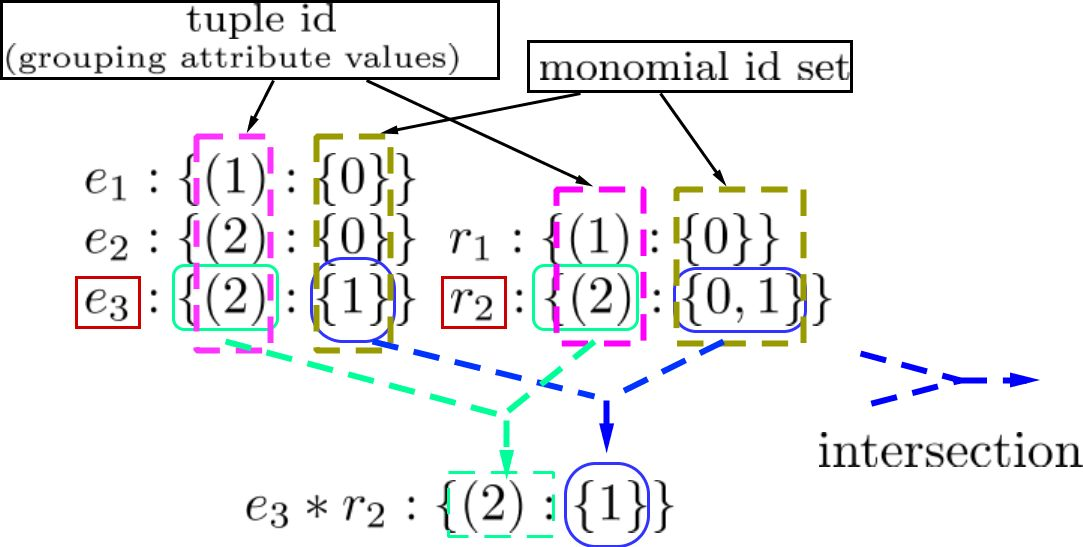
\includegraphics[width=0.4\textwidth,height=0.2\textwidth]{Figures/intersection.jpg}
    \caption{Query provenance index for $Q$, and how to compute coordinate information for $e_3*r_2$ from $V_4(D)$}
    \small \label{fig:query prov index}
\end{figure}
% \begin{figure}
% % \captionsetup[subfigure]{width=1\textwidth}
%      \centering
%     \begin{subfigure}{0.50\textwidth}
%     % \hspace*{-0.8cm}
%         \raisebox{-\height}{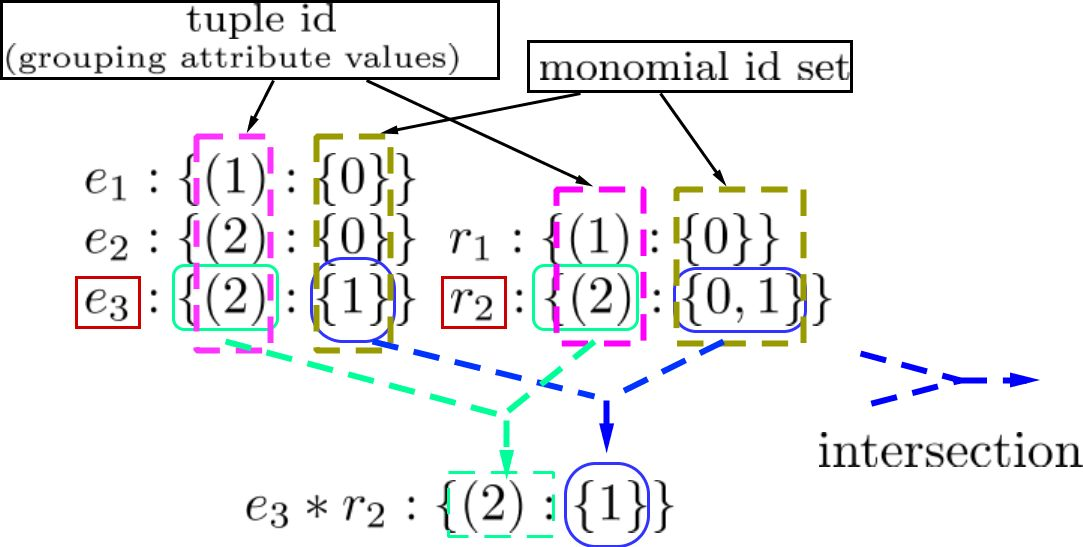
\includegraphics[height = 0.5\textwidth, width=1\textwidth]{Figures/intersection.jpg}}
%         \caption{query provenance index for $Q$ and computing coordinate information for $e_6*r_4$}     \label{fig:stress_test_instance_size}
%     \end{subfigure}
% \end{figure}
% \begin{table}[htp]
% \centering
% \small

% \end{table}

% \begin{table}[htp]
% \centering
% \small
% \caption{The instance of relation $Q_1$ along with how-provenance polynomials}\label{Instance of Q1}
% \begin{tabular}[t]{c|c|c|c|c|c|c|c|} \hhline{~-------}
% &T1&&N1&&COUNT(E)&MAX(L)&\\ \hhline{~-------}
% $t_{q_11}$&1&$\{t_1\}$&MB-203&$\{t_2\}$&1&1&$E_1*T_1$\\ \hhline{~-------}
% $t_{q_12}$&2&$\{t_5\}$&PC-203&$\{t_6\}$&2&3&$E_2*T_2 + E_3*T_2$\\ \hhline{~-------}
% $t_{q_13}$&4&$\{t_9\}$&HP-218&$\{t_6\}$&1&2&$E_4*T_3$\\ \hhline{~-------}
% $t_{q_14}$&5&$\{t_{13}\}$&GK-207&$\{t_6\}$&2&3&$E_5*T_4 + E_6*T_4$\\ \hhline{~-------}
% \end{tabular}
% \end{table}

% \begin{table}[htp]
% \centering
% \small

% \end{table}

% \begin{table}[htp]
% \centering
% \small
% \caption{The instance of relation $V5$}\label{Instance of V5}
% \begin{tabular}[t]{c|c|c|c|c|} \hhline{~----}
% &T1&N1&MAX(L)&\\ \hhline{~----}
% $t_{v_51}$&1&MB-203&1&$\{\{E_1,T_1\}\}$\\ \hhline{~----}
% $t_{v_52}$&2&PC-203&3&$\{\{E_2,T_2\}, \{E_3,T_2\}$\\ \hhline{~----}
% $t_{v_53}$&4&HP-218&2&$\{\{E_4,T_3\}\}$\\ \hhline{~----}
% $t_{v_54}$&5&GK-207&3&$\{\{E_5,T_4\}, \{E_6,T_4\}, \{E_7,T_4\}\}$\\ \hhline{~----}
% \end{tabular}
% \end{table}

% \begin{table}[htp]
% \centering
% \small

% \end{table}

In contrast, since $V_4$, $V_5$ and $V_6$ are aggregate views, we need to compare their how-provenance expressions with the how-provenance of the query to check the {tuple-level conditions}. That can be naively implemented by scanning the entire query provenance for {\em every view mapping} to build satisfiable provenance mappings (Def. \ref{Def: validity condition agg}), which is expensive when $N_{pv}$, $N_{pq}$ and the number of view mappings $m$ are large.  To reduce this cost, we index the query provenance.

\textbf{Query provenance index optimization.} 
% \scream{very long sentence. Please simplify}. 
\eat{Hashmap (mapping the grouping attribute values to the how-provenance monomial set for each query tuple) seems to be helpful to speed up the searching, which, however, still needs to scan the entire query provenance for every view mapping for initialization since the portion of how-provenance monomials in the query {\em involved} in the view mappings may be varied across different view mappings. For example, the view mapping $M_6$ only covers the subgoal $Transcript$ in the query body and thus only the provenance token $r_x (x=1,2,...)$ should be {\em involved} in $M_6$. However, both the token $r_x$ and $e_y$ are {\em involved} in $M_4$ and $M_5$. Such difference can lead to totally different HashMaps and thus inevitable repetitive scans over the entire query provenance for every view mapping in the worst case.}
In order to avoid multiple scans over query provenance, we build an index $I$ for each token in the query provenance to indicate which query tuples (represented by grouping variable values) and which provenance monomials the token is in. The provenance index for $Q$ is shown in Figure \ref{fig:query prov index}. For example, referencing Table \ref{Instance of Q1}, note that token $r_2$ is in the $0^{th}$ and $1^{st}$ monomial in the query tuple $t_{q2}$, which has value $2$ for the grouping variable $G$. So the index for $r_2$ is $r_2:\{(2):\{0,1\}\}$, where $(2)$ represents the tuple id while $\{0,1\}$ is the monomial id set. For a how-provenance monomial in the view, e.g. $e_3*r_2$ in $t_{v_42}$ (with grouping variable value 2), to determine whether it can be mapped to some query provenance monomial, we can retrieve the index for $e_3$ and $r_2$ with grouping variable value $2$ respectively, i.e. $\{1\}$ and $\{0,1\}$, and take the intersection, i.e. $\{1\}$. This indicates that $e_3$ and $r_2$ coexist in the $1^{st}$ monomial of the query tuple with grouping variable value 2 (i.e. $t_{q2}$). 
This derivation process is highlighted in Figure \ref{fig:query prov index}.

We can further optimize the intersection operation by representing the monomial ids with bit arrays, where the $i^{th}$ bit is 0/1 iff a token is/isn't in the $i^{th}$ monomial, and applying bit AND operations. This strategy only requires one full scan over the query provenance to build an index for all view mappings. Details on how to use the index to determine whether provenance mappings from view tuples to query tuple satisfy Def. \ref{Def: validity condition agg} are presented in Algorithm \ref{reasoning_valid_view_mappings}.

\begin{algorithm}[h!] 
\footnotesize
 \SetKwInOut{Input}{Input}
 \SetKwInOut{Output}{Output}
 \Input{a view $V$, a query $Q$, a view mapping $M$ from $V$ to $Q$, query tuple $t_q \in Q(D)$, query provenance index $I$, a set of view tuples $T_v \subseteq V(D)$}

 \Output{Whether provenance mappings from $T_v$ to $t_q$ satisfy Def. \ref{Def: validity condition agg}}
 
\For{$t_v \in T_v$}
{
    Retrieve the provenance monomial set $\Bar{P}$ of $t_v$
    Retrieve the grouping variable values ($Gv$) of $Q$ under mapping $M$

    \For{each provenance monomial $P \in \Bar{P}$}
    {
        \For{each provenance token $p \in P$}
        {
            \If{$p$ is not in $I$ OR $Gv$ is not in the entry of $I$ for $p$}
            {
                \Return false
            }
            
        }
        
        Perform intersection over the index for $p$ with grouping variable values $Gv$
        
        \If{the intersection result is empty}
        {
            \Return false
        }
    }
    
}

\Return true

% {\em Preprocessing step}: Return a set of all possible view mappings $\mathcal{M}$ and the provenance of $Q$

% {\em Reasoning valid view mapping step}: Retrieve provenance of every view. For each query tuple $t$, determine valid view mappings by comparing the provenance of $Q$ and the provenance of $V$

% {\em Covering sets calculation step}: Calculate covering sets by combining valid view mappings for each query tuple.
%  \Return $\mathcal{M}$
 \caption{Checking provenance mappings}
 \label{reasoning_valid_view_mappings}
 \end{algorithm}





\begin{algorithm}[h!] 
\footnotesize
 \SetKwInOut{Input}{Input}
 \SetKwInOut{Output}{Output}
 \Input{a set of valid view mappings $\mathcal{M}$ for query tuple $t \in Q(D)$, query $Q$}

 \Output{a set of covering sets $C$}
 
 For each aggregate term of $Q$, derive a set of view mappings covering it, which forms an array of view mapping sets $S$. 
 
%  Constructing an array of view mapping set $S$ where each view mapping set covers the same aggregate attribute
 
 Determine the order to compute the cross product of every element in $S$
 
 Initialize $C$ as the first view mapping set $s_0$ from $S$.
 
 \For{each set $s\in S - \{s_0\}$}
 {
    
    Initialize cross product result $C' = \{\}$:
    
    \For{each view mapping set $\Bar{M}' \in C$}
    {
        \For{each view mapping $M \in s$}
        {
            get three bit arrays of $\Bar{M}'$ ($M$): $b_1$ ($b_1'$), $b_2$($b_2'$) and $b_3$ ($b_3'$)
            
            construct new view mapping set $\Bar{M}''$ based on the bit OR operation result $b_i \lor b_i' (i=1,2,3)$ and put it into $C'$
        }
    }
    
    
    
    Remove duplicates from $C'$
    
    $C = C'$
    
 }
 
 \caption{Compute covering sets}
 \label{compute_covering_sets}
 \end{algorithm}




\textbf{Materialization and parallelism optimization.} To further improve performance, the provenance of the aggregate views along with the view content can be materialized before the query arrives. The strategy with  materialized view provenance is called {\em eager}, whereas that without is called {\em lazy}. The {\em eager} and {\em lazy} strategies are compared in Section \ref{sec:experiments}. We observe that reasoning about the validity of view mappings is highly parallelizable since the reasoning between different view mappings is independent.
However, since fully parallel computation in a single machine can incur large memory consumption, ProvCite only processes five view mappings at a time. Exploring how to fully develop our system in a distributed environment is left for future work.

% and which can be dealt with by two alternative strategies. One is to pre-compute their how-provenance ({\em eager strategy}) while the other one is to retrieve their how-provenance on the fly ({\em lazy strategy}). Their trade-offs will be discussed in Section~\ref{sec:experiments}.

Using the instances and provenance expressions of $V_4-V_6$ presented in Tables \ref{Instance of V4}-\ref{Instance of V6}, the valid view mappings for every query tuple are presented in Table \ref{Instance of Q1 with view mappings}. Note that for tuple $t_{q2}$, although all of its how-provenance monomials exist in the view tuple $t_{v_52}$, it does not include $e_4*r_2$ which is used to construct $t_{v_52}$, violating the {tuple-level condition}.  Intuitively, since the value of the aggregate term may come from this component of the monomial ($e_4*r_2$), $t_{v_52}$ should not provide citation information for $t_{q2}$.

Finally, valid view mappings are shown in Table \ref{Instance of Q1 with view mappings} along with the query instance, which are then used to compute covering sets for each query tuple in the {\em Covering sets step}. 
\eat{Note that for tuple $t_{{q}3}$, there are two covering sets, $\{M_3\}$ and $\{M_4, M_5\}$;  
% both of these sets cover the aggregate terms in $Q_1$ and are combined using $*$ and $+^R$. % as Table \ref{Instance of Q1 with view mappings} shows. covers both the aggregate terms in $Q1$. 
other combinations of view mappings either {redundantly} or {non-maximally} cover the query's aggregate terms, and therefore are not valid.}


As we observed in \cite{wu2018data}, it is time-consuming to compute {\em all} covering sets. We therefore use two new strategies to achieve speed-up: 1) representing coverings sets using bit arrays; and 2) applying clustering algorithms to avoid an explosion of intermediate results.  These lead to an order of magnitude performance gain (see Section \ref{sec:experiments}).

% \subsubsection{Introducing bit arrays}
\textbf{Bit array optimization.} The computation of covering sets involves merging valid view mappings and removing duplicates, which can be optimized using bit operations. For example, for $Q$, the aggregate term $COUNT(T)$, $MAX(L)$ and $COUNT(E)$ are covered by $\{M_3, M_4, M_6\}$ (denoted by $S_1$), $\{M_3, M_5\}$ (denoted by $S_2$) and $\{M_3, M_5\}$ (denoted by $S_3$) respectively (see Table \ref{Table: view mapping coverage}). We can encode the $0^{th}-3^{rd}$ view mappings $M_3-M_6$ as $\{0,1,2,3\}$, the $0^{th}-2^{nd}$ aggregate terms ($COUNT(T)$, $MAX(L)$ and $COUNT(E)$) as $\{0, 1, 2\}$, and the $0^{th}-1^{st}$ relational subgoals ($Exon$ and $Transcript$) as $\{0, 1\}$.  In this manner, arbitrary view mapping combinations (and thus covering sets) can be represented using three bit arrays in which the $i^{th}$ bit is 1 (0) iff the $i^{th}$ view mapping is included (missing), or the $i^{th}$ aggregated term or relational subgoal is covered (not covered). 
For example, $M_4$ is the $1^{st}$ view mapping, represented by $0100$ (the leftmost bit is the $0^{th}$ bit). $M_4$ covers the $0^{th}$ aggregate term $(COUNT(T))$ and the $0^{th}$ and $1^{st}$ relational subgoals, which are represented by bit arrays $100$ and $11$ respectively. The bit array representations for other view mappings are listed in Table \ref{Table: view mapping}. To compute covering sets, the view mapping combinations from the cross product of $\{S_1, S_2, S_3\}$ (denoted by $S_1 \times S_2 \times S_3$) are considered, which are constructed by applying bit OR operations over the bit arrays from those view mappings. For example, referencing Table \ref{Table: view mapping}, the covering set $\{M_4, M_5\}$ can be constructed by unioning bit arrays $0100$ and $0010$, and the aggregate terms (relational subgoals resp.) jointly covered by them are computed by unioning $100$ and $011$ ($11$ and $11$ resp.). The pseudocode for computing covering sets using bit array representations is presented in Algorithm \ref{compute_covering_sets}.

% To compute covering sets, the cross product of $S_1$ and $S_2$ are computed first, which leads to some view mapping combinations (called {\em sub-covering sets thereafter}) that can cover both the aggregate terms. For instance, $\{M_3, M_5\}$ is one such sub-covering set. The construction of sub-covering sets (and covering sets ultimately) involves merging the view mappings and the aggregate terms and relational subgoals covered by them, which facilitate the following redundancy removal step. For example, $\{M_3,M_6\}$ (picked from $S_1$ and $S_2$ respectively) can jointly cover both the aggregate terms and relational subgoals of $Q$, which, however, is redundant with respect to $\{M_6\}$ (picked from $S_1$ and $S_2$ and one copy is retained) since $\{M_6\}$ is a {\em subset} of $\{M_3,M_6\}$ but still covers the same aggregate terms and relational subgoals as $\{M_3,M_6\}$. So it is safe to remove $\{M_3, M_6\}$ at this point. Then the resulting sub-covering sets are combined with the view mapping set in $S_3$ to compute the final covering sets.

% Note that two key operations are essential in this step, i.e. 1) merging view mappings and the terms covered by them; 2) removing redundancy by subset checking, which can be optimized by applying bit operations.  Three bit arrays are introduced for view mapping combinations, aggregate terms and relational subgoals, in which $i_th$ bit is 0 or 1 if $i_th$ view mapping/aggregate term/relational subgoal is included or missing in the sub-covering set. For example, for sub-covering set $\{M_3, M_6\}$, we use bit array 1001 to represent the view mapping in it (the leftmost 1 is in the 0th bit, which indicates the existence of $M_3$). Similarly, since they cover both the aggregate terms and relational subgoals, the other two bit arrays will be both 11. So when merging sub-covering set (or view mappings) with other sub-covering set (or view mappings), we can apply bit OR operations over the three bit arrays. Similarly, for subset checking operation, bit AND operation is applicable.



% \subsubsection{Applying clustering algorithms}
\textbf{Clustering algorithm optimization.} Since cross product ($\times$) is commutative and associative, different orderings of operands result in the same output but may incur different overhead. For example, with $S_1\times S_2 \times S_3$, if $S_2 \times S_3$ is computed first, the result is $\{M_3, M_5\}$, $\{M_5, M_5\}$, $\{M_3, M_3\}$, $\{M_5, M_3\}$. After removing obvious redundancy, the result is  $\{M_3, M_5\}$, $\{M_5\}$, $\{M_3\}$. Note that $\{M_3, M_5\}$ is a duplicate compared to $\{M_3\}$ since 1) $\{M_3, M_5\}$ and $\{M_3\}$ cover the same set of aggregate terms and relational subgoals (checked by comparing the corresponding bit arrays); and 2) $\{M_3\}$ is a subset of $\{M_3, M_5\}$. It is therefore safe to remove $\{M_3, M_5\}$ since in the final result, any view mapping combinations which include $\{M_3, M_5\}$ will be a duplicate compared to one that includes $\{M_3\}$ and thus won't be a covering set. So the intermediate result of $S_2 \times S_3$ is $\{\{M_3\}, \{M_5\}\}$, which is smaller than the result of the other pairs. This is due to the high similarity between $S_2$ and $S_3$ (actually $S_2 = S_3$). To find good orderings for computing the cross product such that the intermediate result is minimized, clustering algorithms are applied so that view mapping sets which are similar to each other can be clustered and merged first (e.g. $S_2$ and $S_3$). In ProCite, the affinity propagation clustering algorithm \cite{dueck2007non} is used since it does not require a pre-specified number of clusters.
\end{example}
\section{Experiments}
\label{sec:experiments}
\subsection{Experimental set-up}
We implemented \provalg\ in Java 8 using PostgreSQL 9.6.3 as the underlying DBMS. All experiments were conducted
on a Linux server \eat{Distribution? (Gianmaria)}with an Intel(R) Xeon(R) CPU E5-2630 v4 @ 2.20GHz and 64GB of central memory. \eat{claim the use of code from CoreCover algorithm and provide the link to our own code}

{\bf Datasets.} %Three datasets were used in the experiments.
Two realistic datasets were used in addition to GENCODE: 
Hetionet\footnote{\url{https://neo4j.het.io/browser/}} and DBLP-NSF\footnote{\url{https://data.mendeley.com/datasets/ycnngyv5bd}}. 
Summary information of the three datasets, including the number of relations, average size per relation, and the size of the largest relation is presented in Table \ref{Table: datasets_summary}.

We converted Hetionet, which is stored in Neo4j, into a relational database\footnote{Available at 
\url{https://github.com/thuwuyinjun/Data_citation_provenance/files/2417454/hetionet_postgresql.zip}}.
% \scream{Should also make relational representation of Hetionet available.}
% Hetionet aims at building network to systematically identify why drugs work and predict new therapies for drugs. It connects some previously isolated information such as genes, drugs as well as biological processes in which drugs and genes may involve.
DBLP-NSF was developed in \cite{wu2018data}, which integrates DBLP publication information with NSF award information to augment traditional paper citations with funding information.

\begin{table}
\centering
\caption{Summary of datasets}
\small
\begin{tabular}[!h]{|>{\centering\arraybackslash}p{2cm}|>{\centering\arraybackslash}p{1.5cm}|>{\centering\arraybackslash}p{2cm}|>{\centering\arraybackslash}p{2cm}|} \hline
Dataset name& relation \# &average tuple \# per relation& tuple \# of largest relation \\ \hline
GENECODE&7&600k&2000k \\ \hline
Hetionet&38&60k&500k \\ \hline
DBLP-NSF&17&600k&6000k \\ \hline
\end{tabular}
\label{Table: datasets_summary}
\end{table}


{\bf Workloads.} 
We test the performance of \provalg\ using both {\em synthetic} and {\em realistic} workloads. As mentioned earlier, in order to retrieve the provenance of aggregate views, we can use either {\em eager} or {\em lazy} strategy. Plus, index can be built on query provenance. We measure the performance gains by using {\em eager strategy} and query provenance index separately under both workloads. The performance also depends on the {\em policies}. As mentioned in Section \ref{Sec: implementation}, different policies can lead to different results, and can generate either all or some of the covering sets. Due to space limitations, only the case where the {\em all} the covering sets are generated is presented here\eat{do we need to call it full case}.

%only care about t_cs
The purpose of using {\em synthetic workloads} is to determine the key factors which influence performance. 
Extensive experiments were performed in~\cite{wu2018data} measuring the \textit{total reasoning time}  to generate the covering sets ($t_{cs}$) and the \textit{citation generation time}   after covering sets are constructed.  The \textit{citation generation time} is not considered here since \provalg\ only changes how {\em valid view mappings} are determined during covering sets construction process %(rather than {\em formatted citations}) 
relative to the implementations of \rba. Since \provalg\ relies on the query provenance for reasoning, the query time over the provenance-enabled database ($t_{pq}$) is also recorded.
% in~\cite{wu2018data}.


%what key factors can influence the performance
%In terms of $t_{cs}$, based on the experimental results reported in \cite{wu2018data}, 
\eat{Maybe put in a table with these abbreviations in case people forget?}
In \cite{wu2018data}, $t_{cs}$ primarily depends on: 1) the number of view mappings (denoted $N_v$); 2) the total number of predicates under the view mappings (denoted $N_p$); 3) the size of the query instance before duplicates are removed (which is the same as the total number of how-provenance monomials in the query instance $N_{pq}$). The experiments measure the effect of these metrics on $t_{cs}$. %Plus, according to the brief time complexity analysis in Section \ref{Sec: implementation}, 
The total number of how-provenance monomials in the view instance on average ($N_{pv}$) can influence performance according to the analysis in Section \ref{Sec: implementation}, and is also considered in the experiments. So for the experiments for {\em synthetic workloads}, a query generator is built, which can generate random aggregate queries over GENECODE database with $N_{pq}$ how-provenance monomials in total. Given a query $Q$ from this query generator, a view generator can generate $N_v$ views, each of which has $N_{pv}$ provenance monomials in total and has exact one view mapping to $Q$. 

%compare to TLA/SSLA
The trade-offs between \provalg\ and two implementations of the \rba\ proposed in \cite{wu2018data}, TLA and SSLA, are also  measured. 
% We do not consider the {\em pure view-based approach} of \cite{wu2018data},\scream{maybe not correct} since this does not generate fine-grained citations. %;  it is not difficult to extend the view-based approach to handle aggregate queries using conjunctive views. 
As mentioned before, \rba\ can be extended to handle aggregate queries when views are conjunctive views (but not aggregate views). In this case, TLA, SSLA and \provalg\ all generate the same final, fine-grained citations.
%, which derives us to conduct experiments in this setting.

% Plus, according to the complexity analysis in Section \ref{Sec: implementation}, the time to generate covering sets ($t_{cs}$) should also depend on the total number of how-provenance monomials in query and view instance (denoted $N_{pq}$ and $N_{pv}$ respectively) when the views are aggregate views while queries are aggregate queries, which is also experimentally verified herein.

In the {\em realistic workloads}, we use frequent queries against the three databases, and build views to represent the portions of data in the database associated with predefined citations. Both the synthetic and realistic views and queries used are available in our Github repository\footnote{\url{https://github.com/thuwuyinjun/Data_citation_provenance}}. 

To mimic the summary information provided by GENCODE, we defined aggregate views to compute the total number of transcripts per gene, and total number of exons per gene and per transcript. Two additional parameterized views are also defined to represent basic information (e.g. ID, name and type) for each transcript and gene, respectively. The realistic queries  compute the total number of exons ($q1$) and the total number of transcripts per type of gene ($q2$) respectively.

For DBLP-NSF we use the realistic views defined in \cite{wu2018data}. We also add aggregate views to reflect publicly available statistics related to this database, such as the total number of publications per faculty member\footnote{\url{http://csrankings.org/}} and total number of grants per institution\footnote{\url{https://dellweb.bfa.nsf.gov/awdlst2/default.asp}}. Some realistic aggregate queries are designed to represent other summary information, such as total number of publications per institute ($q3$) and total amount of grants per state ($q4$).

Hetionet integrates information from various resources, and includes information about genes, biological process, drugs etc.  This information is stored in different relations in the database. Of these, the biological process relation is associated with citation information (i.e. related publication IDs). After consulting with the authors of Hetionet, two views were defined. The first one is a parameterized view showing the  biological processes that a particular gene is involved in. The second counts the total number of connections between each biological process and corresponding genes by joining several relations, such as the biological process and gene relations.  A typical query ($q5$) counts the total number of connections between each biological process and a certain drug via some genes.


\begin{table}
\centering
\caption{Notation used in the experiments}
\small
\begin{tabular}[!h]{|c|>{\centering\arraybackslash}p{6.8cm}|} \hline
Notation & Meaning \\ \hline
$t_{cs}$&total reasoning time to generate the covering sets for all query tuples \\ \hline
$t_{pq}$&query time over provenance-enabled database \\ \hline
$N_v$&total number of view mappings \\ \hline
$N_p$&total number of predicates under the view mappings \\ \hline
$N_{pq}$&total number of how-provenance monomials in the query instance \\ \hline
$N_{pv}$&total number of how-provenance monomials in the view instance on average\\ \hline
\end{tabular}
\label{Table: notation_summary}
\end{table}

\begin{figure*}
\captionsetup[subfigure]{width=1\textwidth}
     \centering
    \begin{subfigure}{0.30\textwidth}
    \hspace*{-0.8cm}
        \raisebox{-\height}{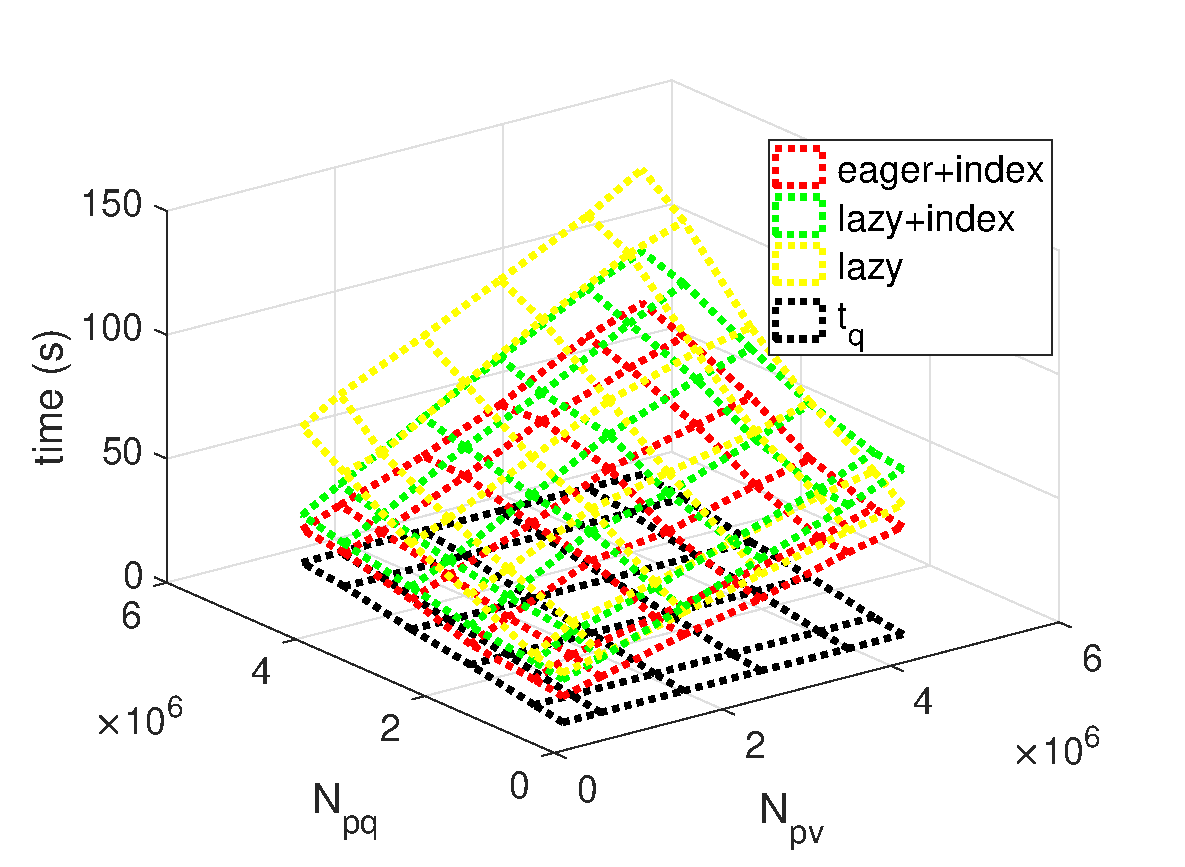
\includegraphics[height = 0.8\textwidth, width=1.2\textwidth]{Figures/synthetic_instance_size.eps}}
        \caption{$t_{cs}$ with varied $N_{pq}$ and $N_{pv}$}     \label{fig:stress_test_instance_size}
    \end{subfigure}
    \hfill
    \begin{subfigure}{0.30\textwidth}
    \hspace*{-0.8cm}
        \raisebox{-\height}{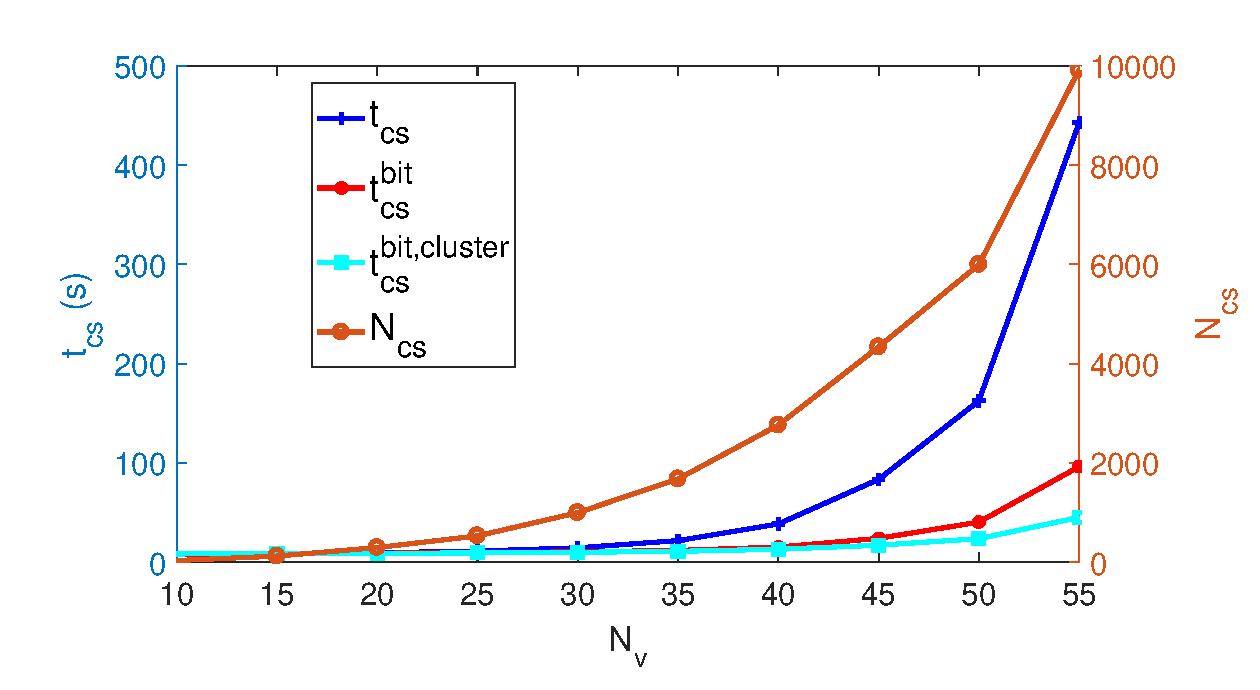
\includegraphics[height = 0.8\textwidth, width=1.2\textwidth]{Figures/synthetic_view_num.eps}}
        \caption{$t_{cs}$ with varied $N_v$}
        \label{fig:stress_test_view_num}
    \end{subfigure}
    \hfill
    \begin{subfigure}{0.30\textwidth}
    \hspace*{-0.8cm}
        \raisebox{-\height}{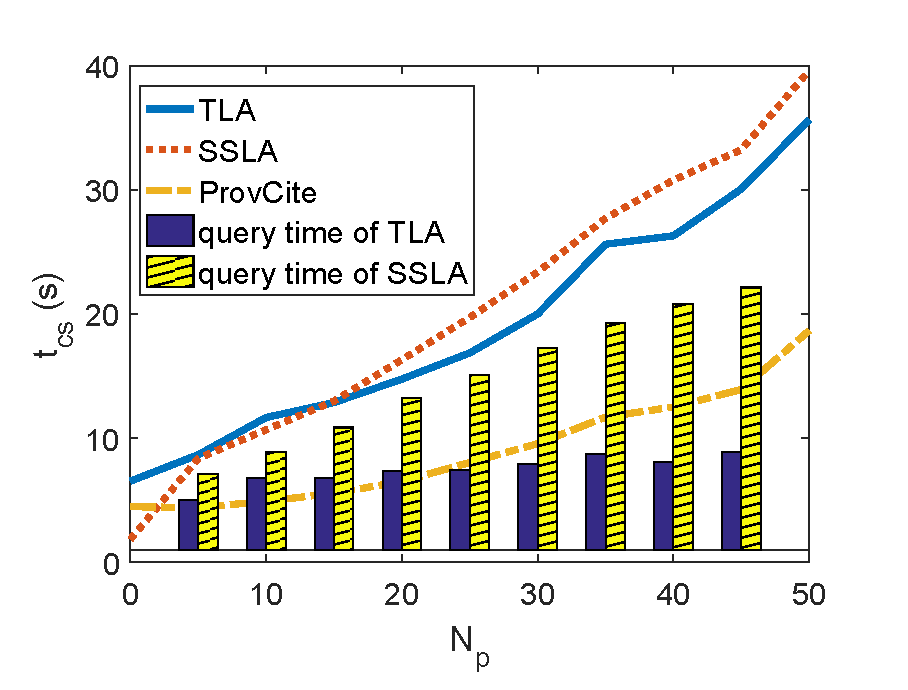
\includegraphics[height = 0.8\textwidth, width=1.2\textwidth]{Figures/synthetic_predicate_num.eps}}
        \caption{$t_{cs}$ with varied $N_p$}
        \label{fig:stress_test_predicate_num_time}
    \end{subfigure}
    \caption{Experimental results for synthetic workloads}
\end{figure*}

Table \ref{Table: notation_summary} provides a summary of the notation mentioned in this subsection.% which will be used in the remainder of this section.

\subsection{Experimental results}
We now report on results from the synthetic and realistic workloads.

\subsubsection{Synthetic workloads} \label{sec: synthetic_exp}
We measured the impact of the size of provenance in both the query and view instances on time performance (Exp1), and the relative performance of \provalg\ and two implementations of the \rba, i.e. TLA and SSLA while varying the number of view mappings (Exp2) and number of view predicates (Exp3).

\textbf{Exp1.}  This experiment measures how the total reasoning time $t_{cs}$ is influenced by the total number of how-provenance monomials in the query instance ($N_{pq}$) as well as 
%the total number of how-provenance monomials 
in the view instance ($N_{pv}$). We randomly generate an aggregate query, and vary $N_{pq}$ by adding appropriate predicates. A fixed number of aggregate views are also generated such that there is exact one view mapping from each of them to the query and the total number of view mappings is fixed at 20. \scream{claim view number here} In practice, the number of views that touch the query is usually far smaller than the total number of views. So 20 is a pretty large number. Both $N_{pq}$ and $N_{pv}$ are varied from 50K to 5M. $t_{cs}$ is measured for different ($N_{pq}$, $N_{pv}$) pairs under the {\em eager} and {\em lazy} strategy with query provenance index and the {\em lazy} strategy without index.  

\textbf{Results.} 
The time performance, $t_{cs}$, is shown using 3D surfaces in Figure \ref{fig:stress_test_instance_size}, with the eager strategy with index, lazy strategy with index and pure lazy strategy shown in yellow, blue and black respectively. Plus, the time query against the provenance-enabled database is also recorded with green surface. It shows that the query provenance index can lead to about 1.0x-1.8x speed-ups by comparing lazy strategy with index and pure lazy strategy while materializing view provenance results in about 1.1x-1.5x speed-ups by comparing eager strategy and lazy strategy with index. In the end, the combinations of the index and eager strategy leads to up to 2x performance gains. Besides, the result also implies scalability of our approach since it only takes less than 2 mins to process query instance with up to 5 million how-provenance monomials and 20 views with up to 5 million how-provenance monomials, which rarely happens in practice. We also observe that reasoning about valid view mappings is highly parallelizable, which means that further improvement can be achieved by implementing in distributed systems. 

% We also measured the extra space needed for the eager strategy, where the provenance of views is precomputed and stored in the database; it takes about 180 MB in the database to store the provenance for each view when the instance of the view includes up to 1 million how-provenance monomials. 

\textbf{Exp2.} The goal of this experiment is to compare the relative performance of \provalg, TLA and SSLA while varying the number of view mappings ($N_v$). Since TLA and SSLA cannot handle aggregate views, only conjunctive views are used. So there is no difference between {\em eager} and {\em lazy} strategy and the query provenance index is not useful since the provenance of views is not necessary. But the effect of two optimization strategies on covering set computation, i.e. applying bit arrays and clustering algorithms are measured here. The query is a fixed aggregate query with 1 million how-provenance monomials in its instance. $N_v$ is varied from 1 to 50 and there are no predicates or lambda variables for each individual view. 

\textbf{Results.}
The experimental results are presented in Figure \ref{fig:stress_test_view_num}, which shows the change of $t_{cs}$ for ProvCide and the number of covering sets ($N_{cs}$) with the increase of the number of view mappings ($N_v$) with and without using bit arrays and clustering algorithm. We observe that TLA and SSLA have almost the same performance as ProvCite and thus are not presented here. Figure \ref{fig:stress_test_view_num} indicates that when $N_v$ is large, an exponential number of covering sets are generated, which leads to inevitable bad performance (see blue line). But bit array computation and the use of clustering algorithm lead to about 5 times and about 2 times speed up respectively and order of magnitude performance gains can be achieved in the end.


\textbf{Exp3.} In this experiment, \provalg\ is compared with TLA and SSLA while varying the total number of predicates ($N_p$) in views. Similar to Exp2, the query is an aggregate query which can generate about 1 million tuples. The number of view mappings is fixed at 10 and there are initially no predicates. At each run, one more local predicate is added. As shown in \cite{wu2018data}, increasing $N_p$ can significantly influence the performance of TLA and SSLA by 1) increasing the query time since the query is extended to explicitly evaluate the satisfiability of predicates of the views in the query instance; 2) increasing the number of {\em reasoning groups} since we need to compute covering sets for each group and thus more {\em reasoning groups} in the query instance means more reasoning time. In theory, \provalg\ will also suffer from a large number of groups but will save on query time.

\textbf{Results.} The experimental results are shown in Figure \ref{fig:stress_test_predicate_num_time}, which matches the analysis above. As the number of predicates increases, $t_{cs}$ 
increases slowly for \provalg. In contrast, TLA and SSLA are twice as slow as \provalg\ for large $N_p$. To understand the reason for this, the query time for TLA, SSLA and ProvCite is also presented in this figure, which implies that the increasing query time becomes the major overhead for both TLA and SSLA, thus slowing down the computation.

{\bf Discussion.} The experiments reveal that all four metrics, $N_{pq}$ (the total number of how-provenance monomials in the query instance), $N_{pv}$ (the total number of how-provenance monomials in the view instance on average), $N_v$ (the total number of view mappings), $N_p$ (the total number of predicates under the view mappings) can affect the total reasoning time $t_{cs}$. In extreme cases, where the value of the metric is very large, bad performance is unavoidable when ProvCite is implemented naively, which, however, can be substantially improved by the use of various optimization strategies. We therefore expect better time performance for realistic workloads where the extreme value of those metrics rarely appear. 

% In the case of aggregate views where how-provenance is necessary, the  eager strategy beats the lazy strategy in terms of time.  The speedup is small (10\%-40\%), however, extra space is needed (up to 180 MB per view). So in practice, the choice between the eager or lazy strategy depends on whether speed or space is more important. In comparison to the previous approaches, TLA and SSLA, \provalg\ is not only more powerful in that it supports aggregate views but is also (surprisingly) frequently more efficient.  

\subsubsection{Realistic workloads}
\label{ssec: realistic}
The experimental results for realistic workloads are presented in Table \ref{Table: realistic_performance}, which includes the time to generate covering sets ($t_{cs}$) for three cases (lazy, lazy + index and eager + index), as well as the metrics that can potentially affect the performance: the total number of how-provenance monomials in the query instance ($N_{pq}$), the total number of view mappings ($N_v$), the total number of predicates in the views under all the view mappings ($N_p$) and the time to query the provenance along with the instance. Except for $q1$, $t_{cs}$ is less than 10 seconds for all queries. Although $N_{pq}$ is more than one million in $q1$, the total reasoning time ($t_{cs}$) is only about 11-13 seconds for the three strategies, which is acceptable considering the large query instance. Note that index does not always help since 1) it takes significant time to build the index for query provenance (e.g. up to 3 seconds for $q1$) and 2) when indexes are not used, the small number of view mappings leads to weak effect of multiple scans over entire the query provenance. But according to Section \ref{sec: synthetic_exp}, index can provide better scalability and thus it will be more efficient to deal with possible extreme cases in practice. We also list the query time over the provenance-enabled database in the last column, which indicates that the reasoning time ($t_{cs} - t_{pq}$) is almost the same as $t_{pq}$. So it is possible that when users are browsing the query result, the system can generate covering sets for all query tuples in the back-end, ready to instantly construct formatted citations when users select tuples of interest.

\eat{Comparing to time to simply generate query instance (See last column), $t_{cs}$ is still reasonable considering the large instance. When users are browsing the query result, the system can generate covering sets for all query tuple in the back-end, ready to construct formatted citations when users select tuples of interest.}

{\bf Discussion.} The experimental results above show that reasonable time performance can be guaranteed in practice where none of the crucial metrics become too large.  Revisiting the experimental results for synthetic workloads, when the total number of how-provenance monomials in the query instance ($N_{pq}$) is more than 1 million (as in $q1$), the reasoning time ($t_{cs}$) can be large (up to 150 seconds). However, the time shown for $q1$ is significantly smaller since the number of view mappings ($N_v$) is only 1, and the reasoning time relies on both $N_v$ and $N_{pq}$.




\begin{table}
\centering
\caption{Experimental results on realistic datasets}
\small
\begin{tabular}[!h]{|>{\centering\arraybackslash}p{0.75cm}|>{\centering\arraybackslash}p{0.85cm}|>{\centering\arraybackslash}p{0.85cm}|>{\centering\arraybackslash}p{0.85cm}|>{\centering\arraybackslash}p{0.7cm}|>{\centering\arraybackslash}p{0.25cm}|>{\centering\arraybackslash}p{0.25cm}|>{\centering\arraybackslash}p{1cm}|} \hline
Query& $t_{cs}$ (s) (eager + index) & $t_{cs}$ (s) (lazy + index)& $t_{cs}$ (s) (lazy)& $N_{pq}$&$N_v$&$N_p$& $t_{pq}$(s) \\ \hline
$q1$&11.05&12.93&11.89&1237k&1&0&5.09 \\ \hline
$q2$&1.75&2.06&3.26&203k&2&0&0.69 \\ \hline
$q3$&4.95&6.62&6.44&507k&2&0&2.92 \\ \hline
$q4$&5.90&6.49&6.33&416k&1&0&2.80\\ \hline
$q5$&4.65&5.10&4.81&243k&3&0&2.32 \\ \hline
\end{tabular}
\label{Table: realistic_performance}
\end{table} 



\section{Conclusions}\label{sec: conclusion}
This paper builds on the connection to {\em data provenance} to develop a model for  data citation which is able to handle aggregate queries and views. The model reasons about citations at the level of tuples in the query result using provenance to enable citations to arbitrary subsets of the query result. 

The \pbafull\ was implemented in \provalg, and extensive experiments conducted under both {\em synthetic} and {\em realistic workloads}.  The results show that \provalg\ can not only handle a larger class of queries than pure Rewriting-based approaches (which assume conjunctive queries and views, e.g. \cite{wu2018data}), but is much faster in some cases.  However, the approach assumes a \textit{provenance-enabled DBMS}.
Trade-offs between an {\em eager} versus {\em lazy} strategy for generating view provenance was also explored.  The choice involves a trade-off between speed and space.

In future work, we would like to explore how to insert data citation into the  larger citation ecosystem involving bibliometrics. We would also like to explore how to combine data citation with machine learning algorithms by leveraging \pba, which can be simply achieved by viewing machine learning model as an aggregate function.
\eat{
This is the first paper to build a {\em \pbafull} to connect the notion of {\em data citation} and {\em data provenance}, which is able to handle a larger class of queries and views i.e. aggregate queries and views compared to previous work and generate citations for query result at \textit{various granularity}. Efficient implementations for provenance reasoning, \provalg, are challenging but achieved by utilizing various optimization strategies. In \provalg, two different strategies are designed to deal with the provenance of views, which is either precomputed ({\em eager strategy}) or computed on the fly ({\em lazy strategy}). 

Extensive experiments are conducted under both {\em synthetic workloads} and {\em realistic workloads}. The experimental results justify the feasibility of \provalg\ to this model, which is not only powerful but also much faster in some cases compared to the implementations of \rba. Besides, the trade-offs between {\em eager strategy} and {\em lazy strategy} has been explored. The choice depends on users' preferences for speed or less space in practice.

In future work, we would like to explore how to integrate data citation into a larger citation ecosystem, which aims at efficiently and accurately computing and monitoring contributors' bibliometrics. Plus, considering the fact that machine learning algorithms are widely used and cited in {\em data science environment} and machine learning model is a special aggregate function, it will be also an interesting extension to automate citation generation process for machine learning pipeline.}
% \section{Optimizations in detail}
\subsection{Optimization on determining valid view mappings}
\subsubsection{Building indexes for query provenance}

Recall that the validity of view mapping $M$ for each query tuple $t_q$ depends on the mapping from a (or multiple) how-provenance monomial(s) of the view tuples to those of query tuple $t_q$. A naive solution is simply to scan the entire query provenance (at least once) for {\em every view mapping} to attempt to map every view provenance to the query provenance, which is expensive especially when $N_{pv}$ and $N_{pq}$ are large. Hashmap (mapping from the grouping attribute values to the how-provenance monomials in the query) seems to be helpful to speed up the searching, which, however, still needs to scan the entire query provenance for every view mapping. This issue is presented as below.

\begin{example}
Consider the following query:
\begin{tabbing}
$Q(G, COUNT(T), MAX(L)):-Exon(E, L, T'), E <= 6$\\
\tab\tab\tab\tab$Transcript(T, N, Ty, G), T = T'$
% \tab\tab\tab$$
\end{tabbing}

Its instance along with the how-provenance polynomials are presented in Table \ref{Instance of Q}. By referencing the views defined in \ref{}, $V4-V6$ can potentially provide view mappings for $Q$. So their instance and how-provenance expressions are shown in Table \ref{Instance of V4'} to Table \ref{Instance of V6'}.

\begin{table}[htp]
\centering
\small
\caption{$Q(D)$ with how-provenance polynomials}\label{Instance of Q}
\begin{tabular}[t]{c|c|c|c||b|} \hhline{~----}
&G&COUNT(T)&MAX(L)&prov\\ \hhline{~----}
$t_{q1}$&1&1&1&$e_1*r_1$\\ \hhline{~----}
$t_{q2}$&2&2&3&$e_2*r_2 + e_3*r_2$\\ \hhline{~----}
$t_{q3}$&3&3&3&$e_4*r_3 + e_5*r_4 + e_6*r_4$\\ \hhline{~----}
\end{tabular}
\bigskip
\caption{$V_4(D)$ with how-provenance polynomials}\label{Instance of V4'}
\begin{tabular}[t]{c|c|c||b|} \hhline{~---}
&G1&COUNT(T1)&prov\\ \hhline{~---}
$t_{v_41}$&1&1&$e_1*r_1$\\ \hhline{~---}
$t_{v_42}$&3&3&$e_4*r_3 + e_6*r_4 + e_7*r_4$\\ \hhline{~---}
\end{tabular}
\bigskip
\caption{$V_5(D)$ with how-provenance polynomials}\label{Instance of V5'}
\begin{tabular}[t]{c|c|c||b|} \hhline{~---}
&G1&MAX(L)&prov\\ \hhline{~---}
$t_{v_51}$&1&1&$e_1*r_1$\\ \hhline{~---}
$t_{v_52}$&2&3&$e_2*r_2 + e_3*r_2$\\ \hhline{~---}
$t_{v_53}$&3&3&$e_4*r_3 + e_5*r_4 + e_6*r_4 + e_7*r_4$\\ \hhline{~---}
\end{tabular}
\bigskip
\caption{Instance of relation $V6(D)$ with provenance}\label{Instance of V6'}
\begin{tabular}[t]{c|c|c||b|} \hhline{~---}
&G&COUNT(T)&prov\\ \hhline{~---}
$t_{v_61}$&1&1&$r_1$\\ \hhline{~---}
$t_{v_62}$&2&1&$r_2$\\ \hhline{~---}
$t_{v_63}$&3&2&$r_3 + r_4$\\ \hhline{~---}
\end{tabular}


\end{table}

There is an obvious view mapping from each view $V4-V6$ to $Q$, denoted as $M4-M6$, which should satisfy the {\em schema-level conditions} by comparing the grouping variables and aggregate variables between the views and the query. Then the {\em tuple-level conditions} are checked by comparing the how-provenance of each view tuple and that of each query tuples, As claimed earlier, a hashmap $HM$ is built to store the provenance information, in which the key-value pair stores the grouping attribute value and the set of how-provenance monomials respectively for each query tuple. For example, for query tuple $t_{q2}$ in the query $Q$, the entry in $HM$ corresponding to this tuple will be $\{2\rightarrow \{e_2*r_2, e_3*r_2\}\}$ (denoted by $En$) where $2$ is the value for grouping attribute $G$ while $\{e_2*r_2, e_3*r_2\}$ is the how-provenance monomial set for $t_{q2}$. For a view tuple (e.g. $t_{v_52}$), in order to build the potential monomail mappings for its how-provenance monomial, we firstly retrieve the {\em candidate entry} (e.g. $En$ for $t_{v_52}$) from $HM$ with the value of the grouping attributes (that are mapped to the grouping attributes under the view mapping). Then for every monomial of this view tuple (e.g. $e_2*r_2$), we can check its existence in the candidate entry (with $O(1)$ time for every monomial) and thus determine whether the provenance monomial mappings satisfy the validity conditions

However, it is worth noting that $HM$ is not helpful for determining the validity of $M6$ since the how-provenance monomials in $V6(D)$ only include one provenance token (e.g. see tuple $t_{v_62}$, it includes on provenance monomial $r_2$), for which we cannot determine their existence in some entry in $HW$ in $O(1)$ time. For example, the {\em candidate entry} for $t_{v_62}$ is still $En$, but $r_2$ is not the same as either of the two monomials in the monomial set ($e_2*r_2$ and $e_3*r_2$), which, however can be mapped to either $e_2*r_2$ or $e_3*r_2$ under view mapping $M6$ according to the validity conditions. So we either need to consume more time for search in $HW$ or have to reconstruct another hashmap $HW'$ which simply includes the portion of how-provenance monomials involved in $M6$ (such that the search takes only $O(1)$), either of which case can result in another full scan of the entire query provenance.

In order to avoid multiple scans over query provenance, we built an index $I$ for each single provenance token to indicate which query tuples (represented by grouping attribute values) and which provenance monomials it lies in. For example, for token $r_4$ in the query provenance, since it is in the second and third monomial in the query tuple $t_{q3}$, such {\em coordinate information} is thus stored in the index $I$ taking $r_4$ as the key. For a how-provenance monomial in the view, e.g. $e_4*r_3$ in $t_{v_42}$, to determine whether it can be mapped to some query provenance monomial, we can retrieve the {\em coordinate information} for $e_4$ and $r_3$ respectively (if any) and then perform intersection over the {\em coordinate information} of the two tokens to check whether they coexist in some how-provenance monomial in the query provenance. For instance, after taking the intersection operations, the common position for $e_4$ and $r_3$ is the first monomial in the tuple $t_{q3}$. We can further optimize the intersection operations by representing the monomial coordinate with bit array and applying bit AND operations for speed-ups. It turns out that this strategy only requires full scan over the query provenance for all the view mappings.

\subsubsection{Parallelly determine valid view mappings}
We also observe that the validity of one view mapping is independent from others, which thus drives us to parallelize the computation. One straightforward way is to create one thread for each view mapping, which, however can degrade the performance due to the overhead to retrieve the view provenance from the database and the memory consumption in each thread. After trial and errors, we find that batch processing 5 view mappings each time can lead to best performance. Note that the system is built on single machine, it is worth trying to migrate it to distributed systems for further performance gains in the future.



\subsection{Optimization on computing covering sets}
As we observed in \cite{wu2018data}, it is a time-consuming step to compute {\em all} covering sets after the validity of view mappings are determined. Compared to \cite{wu2018data}, two strategies are applied to speed up the covering sets calculation, i.e. 1) representing coverings sets using bit arrays; 2) applying clustering algorithms to avoid an explosion of intermediate results. 

\subsubsection{Introducing bit arrays}
The computation of covering sets involves merging valid view mappings by each every aggregate term incrementally and removing duplicated view mapping combinations by comparing the aggregate terms and subgoals that are jointly covered by the view mapping combinations. For example, for $Q$, the aggregate term $COUNT(T)$ is covered by $\{M_3, M_4, M_6\}$ (denoted by $S_1$) while $MAX(L)$ is covered by $\{M_5, M_6\}$ (denoted by $S_2$). By considering all the view mapping combinations in the cross product of $S_1$ and $S_2$, 


\subsubsection{Applying clustering algorithms}



\eat{; and 3) query tuples associated with the same set of valid view mappings form a {\em reasoning group} to avoid repetitive computations of covering sets. For example, $t_{q1}$ and $t_{q2}$ have the same set of valid view mappings, $\{M_5\}$, which should end up with the same covering sets. So those two tuples are grouped together to compute covering sets once. These optimizations can result in orders of magnitude speed-up.} %However, due to the space limit, the details are not provided here. 



\end{example}
%ACKNOWLEDGMENTS are optional
\section{Acknowledgments}
This research was partially funded by NSF IIS 1302212 NSF ACI 154736, Israel Innovation Authority, the Israel Science Foundation, and Len Blavatnik and the Blavatnik Family foundation. The authors thank Peter Buneman for conceiving the idea of data citation, and Val Tannen for discussions on query rewriting and provenance.
%; and Boris Glavic for his support in understanding details of GProM's source code.


% The following two commands are all you need in the
% initial runs of your .tex file to
% produce the bibliography for the citations in your paper.
\newpage
\balance
\bibliographystyle{abbrv}
\bibliography{vldb_sample}  % vldb_sample.bib is the name of the Bibliography in this case
% You must have a proper ".bib" file
%  and remember to run:
% latex bibtex latex latex
% to resolve all references

% \subsection{References}
% Generated by bibtex from your ~.bib file.  Run latex,
% then bibtex, then latex twice (to resolve references).

%APPENDIX is optional.
% ****************** APPENDIX **************************************
% Example of an appendix; typically would start on a new page
%pagebreak
\clearpage

% \begin{appendix}
Subject: Submission of revised paper 360

Dear VLDB Program Committee:
Thank you for the decision requesting a revised version of our paper for a second evaluation. We have carefully reviewed the feedback and comments, and have revised the manuscript as detailed below. The reviewers mainly criticized the problem motivation (Section 1 and Section 3), implementation and optimization (Section 5) and experiments (Section 6), which we addressed by 1) improving the motivation on why we should care about aggregation in data citation, 2) adding a detailed comparison between the algorithms proposed in this paper and our previous work to highlight the need to use provenance; 3) adding implementation and optimization details; and 4) refining the experiments to show the effect of the optimizations.
 
% We look forward to hearing from you!
% Sincerely,
% Authors of Paper 360

\section{Response to Reviewer 1}
% \textbf{W1}. 
% It is a rather incremental paper, compared to \cite{alawini2018data} and \cite{wu2018data}. The underlying ideas were already known and previous systems showed feasibility (to some extent).

\textbf{Response to W1}: Thanks for your concerns about the novelty of this paper. We agree with you that some of the underlying ideas were discussed in our previous work. However, this work is new compared to those papers since 1) we develop a new model for data citation based on provenance. Compared to \cite{alawini2018data} and \cite{wu2018data}, the novelty of this paper is that it can support aggregate queries and aggregate views, which was not addressed in \cite{alawini2018data} and \cite{wu2018data}. To motivate the use of provenance In Section 3.3, we compare \pba\ and \rba\ from \cite{wu2018data} via an example to show why the previous solutions and their extension fail in the context of aggregate queries with aggregate views, thus motivating the need for provenance. 2) the implementation, which is presented in Section 5.2 along with optimizations for performance improvement,  is totally different from our previous system. The optimization strategies include the use of indexes over query provenance and materialized view provenance for reasoning about valid view mappings, and the use of bit arrays and clustering algorithms for computing covering sets. These optimizations are new to this work, and have not been published in our prior work. Some optimization ideas can also be used in other applications, as discussed in the conclusions.

% \textbf{W2}
% . Some optimizations are mentioned that are claimed to "result in orders of magnitude in speed-up". This is not substantiated in the experimental section.
\textbf{Response to W2}:
We agree, and thanks for pointing this out. We have reorganized the paper so that there is room to present both details of the optimizations and the related experimental results (see Sections 5.2 and 6.2 respectively). The optimization strategies include two parts: The first one is for the reasoning step, which includes building indexes over the query provenance and materializing the view provenance.  The second is for the covering set step, which includes representing covering sets with bit arrays and applying a clustering algorithm to minimize the size of intermediate results during the computation. More details can be found in Exp2 of Section 6.2, where the optimization strategies for the covering sets step are shown to result in an order of magnitude speed-up (see Figure 2(b)).

% W3. It seems "early" to start looking at extensions of the prov+rewriting approach while the non-aggregate case is in its infancy. It is unclear how the proposed techniques help to speed up the simpler case. 
\textbf{Response to W3}: 
As we now better explain in the paper, the primary motivation for using provenance is not to speed-up the process, but rather to support aggregate queries and views for which provenance is necessary. We explain why aggregate queries and views are increasingly important in Section 1 by discussing two datasets, Hetionet and GENCODE.  In Section 3 we explain why provenance is necessary to deal with aggregate queries and views.  Since dealing with provenance is known to be costly, the optimization efforts described in Section 5 are necessary to obtain ``acceptable'' performance, i.e. performance that is comparable to the previous solution for the non-aggregate case. As Section 6.2 shows, in some cases (Exp3), PBM can even outperform RBM since the query in RBM used for evaluating the view predicates when retrieving the query instance is more expensive than the query in PBM used for retrieving the query instance along with the provenance.
While we agree there is certainly more to be done for the non-aggregate case, looking at the aggregate case significantly increases the applicability of the solution to realistic cases. 

% W4. Some comparisons are made with two competitors (from [35]), but insufficient details are provided to understand the experiments.

\textbf{Response to W4}:
We agree that in the first version of our paper, we failed to elaborate on the differences between PBM and RBM. In order to remedy this, we rewrote Section 3 to present some important details of RBM using a running example, show the key differences between RBM and PBM and explain why RBM fails for aggregate queries with aggregate views. We also highlight in Section 5.2 (in the first paragraph of the right column of page 8) the fact that PBM and RBM have different mechanisms for the case of conjunctive views. We believe that these details on the implementation differences between RBM and PBM are necessary to understand the effect of the experiments.

In the experimental section (Section 6), we also present more details to show the effect of the optimization strategies introduced in Section 5 (Exp1, Exp2) and show how PBM can outperform RBM in some cases (Exp3). In Exp1, we show experiments in the case of aggregate queries and aggregate views, which cannot be handled by RBM. So there is no comparison between them in Exp 1. In Exp2, the goal is to compare PBM and RBM by the increasing number of conjunctive views and showing the effect of the optimization strategies for the covering set computation. We observe that the time to compute covering sets becomes the major overhead for both PBM and RBM and thus the differences between them become insignificant; thus only the experimental results for PBM are shown in Figure 2(b). In Exp3, the number of predicates varies in the case of conjunctive views, in which case PBM can outperform RBM. As indicated in Section 6.2, the reason behind this is that the query for retrieving the provenance and query instance in PBM incurs less overhead than the query for evaluating the view predicates explicitly in RBM.

% C1. Originality is low, however: the validity conditions are what one would expect and are obtained by inspecting whether sufficient information is present in views to deduce information for the query result tuples.
\textbf{Response to C1}:
It is true that we take a lot of effort to formalize the (intuitively reasonable) validity conditions for view mappings in the context of aggregate queries and possible aggregate views, which is the main contribution in this paper. However, implementing the model to perform in an acceptable time is also a major contribution, and one which we were not initially convinced could be done.  To that end, significant engineering efforts were required and optimizations developed to speed up the reasoning process.  We now expand on these optimizations in the revised paper.  Note that several of these techniques can be used in other applications, although we do not have space to expand on this idea and mention it only in the conclusions. For example, the index over query provenance is applicable to speed up the computation where we need to compare the provenance of two queries, such as linked brushing in interactive data visualizations \cite{psallidas2018smoke}, which is highlighted in the conclusions of the paper.

% C2. Section 5.2 in the paper is a bit strange; its title contains the word "optimization" but apart from a short paragraph listing optimization strategies no details are given. It is also not reported in the experimental section what impact these optimizations have on performance.
% Nevertheless, it is claimed that these optimizations "can result in orders of magnitude speed-up". This claim should be experimentally substantiated a more in-depth discussion of the optimization techniques should be present.


\textbf{Response to C2}:
Good point. To deal with this issue, we provide more details on the optimizations strategies in both the reasoning  and covering set steps in Section 5. In order to optimize the reasoning step, we build an index over query provenance to speed up comparisons between the query provenance and view provenance. The view provenance can also be materialized to avoid repeated re-computation. As shown in Exp1 in Section 6.2, these optimizations can lead to up to 2x speed-up. 

For the covering set step, we use bit arrays to represent each covering set and the subgoals and aggregate terms it covers. We also observe that in the process of producing covering sets, different orders of combining valid view mapping sets have different performance due to the size of intermediate results. A clustering algorithm called Affinity propagation is therefore applied to compute the best order. The two optimization strategies can result in 5x and 2x improvements, respectively, and their combination can lead to an order-of-magnitude speed-up as shown in Exp2 in Section 6.2. 

% C3. In addition, a comparison with two previous approach TLA and SSLA (from \cite{wu2018data}) is included. Since no details are provided about these two competitors, it is difficult to assess with what is compared here. These comparisons are a bit "internal", meaning that they are perhaps more of interest to the authors (since the competitors originated from same research groups as the authors), rather than of interest to a wider audience.
\textbf{Response to C3}:
Thanks for your comments. To solve this issue, we modified Section 3 to use a running example to illustrate briefly how to use TLA and SSLA for citation reasoning, highlighted the implementation differences between RBM and PBM when dealing with conjunctive views in Section 5.2 (in the first paragraph of the right column of page 8) and showed how such implementation differences lead to different overhead in Section 6.  

We agree that those comparison seems a bit ``internal'', however there are no other approaches to include in the comparison at this point. The comparison between PBM proposed in this paper and RBM proposed in our previous paper is still necessary since it gives reader a sense of the trade-offs between PBM and RBM, and thus provides some insight on which one should be used in different scenarios or workloads. 

% D1 sect 3.1. Use initial capital letters for transcript2tag and exon2tag.
\textbf{Response to D1}:
Thanks, it has been revised.

% \textbf{Response to D2} sect 3.2. you define valid in terms of visibility; it is unclear, however, what being visible means, until much later. Similarly, for being ``involved''. The explanation given here could be improved.
\textbf{Response to D2}: Thanks for your comments, we modified the terminology in that paragraph. Instead of talking about ``visibility'',  we say ``for a query tuple $t$, view mapping $M$ is valid iff some portion of $t$ appears in the instance of $V$ under $M$'', which is determined by examining the lambda variables, the head variables and the predicates of views in the query. To illustrate this point, we use a modified example in Section 3.2 to show what kinds of query tuples can appear in the view instance under certain view mapping $M$, and thus when $M$ is valid for such query tuples. In the same example, we also briefly introduce how RBM determines the validity of view mappings in the implementation, which is mainly achieved by evaluating the view predicates along with query evaluation. 
Also we removed the sentence with the word ``involved'', which is used for illustrating the concept of ``covered''. We delay the discussion about this point until Section 4.

% D3 sect 3.3. What happens if Tid <=5 in the query. It would be instructive to have an example in which the view does not hold all necessary information.
\textbf{Response to D3}:
We have modified the example in Section 3.3 to illustrate this, where the view mapping of $V_2$, $M_{22}$ is not valid for query tuple $t_{{q_2}2}$; this is also justified in Section 4.3.2. The invalidity is because tuple $t_{q_{\ref{eg: illustrative_eg3}}2}$ does not include the how-provenance token $g_4$ as the view tuple $t_{v_21}$ does, which is filtered out by the predicate $Gid \leq 3$. As a comparison, in Section 4.3.2, we also show that if the predicate is relaxed to $Gid \leq 4$, then the token $g_4$ is included in tuple $t_{q_{\ref{eg: illustrative_eg3}}2}$, thus satisfying the tuple level conditions in Def. \ref{Def: validity condition agg}. However, if tuple $t_{q_{\ref{eg: illustrative_eg3}}2}$ includes a token that is not in view tuple $t_{{v_2}1}$, then then tuple level condition still does not hold. This is the idea of ``exact match'' between query provenance and view provenance.

% D4 sect 3.3. Table 5: How are Lee, Joe and Liu?
\textbf{Response to D4}:
It should be \{Group: [`Lee', `Joe', `Liu']\} after applying the citation construction policies, which simply aggregates all the values of the same key (i.e. Group) from different view tuples. In Section 3.3, we changed the example for the purpose of clarifying the mechanism of RBM and to show why we need provenance for aggregate queries in the case of aggregate views. However,  citations for the query tuples are still presented. 
% D5 sect 6.1., last sentence: notation "used" in

\textbf{Response to D5}: Done

% D6 sect 6.2.1. exp 3. The explanation of the discrepancy between Provcite and TLA/SSLA is not clear enough.

\textbf{Response to D6}: 
In order to clarify the mechanism of TLA and SSLA, we rewrote Sections 3.1 and 3.2 to show how TLA/SSLA deal with simple conjunctive queries and how they can be extended to deal with aggregate queries for conjunctive views. We also explain how ProvCite deals with simple conjunctive queries and conjunctive views with provenance in Section 5.2 (in the first paragraph of the right column of page 8), and highlight the implementation differences between TLA/SSLA and ProvCite.


\section{Response to Reviewer 2}

% W1 Novelty and technical contribution might be considered a bit narrow in terms of improvements over the authors' previous work and over existing solutions for data citation
\textbf{Response to W1}:
As we now better explain, the novelty of our paper has two aspects: 1) we formalize the connections between provenance and data citation, and apply this connection to address data citation for aggregate queries and views, which has not been completely studied; 2) we apply various optimizations to gain performance.  These techniques may be applicable in other areas.  For example, due to the close connection between data citation and fine-grained access control, our techniques are applicable in the fine-grained access control. In addition, as we mention in the paper, the key step in determining the validity of view mappings is to compare the provenance of the input query and the views, which indicates that our techniques and optimization ideas (especially the query provenance index idea) are usable for any application where the reasoning needs to compare provenance between different queries or views. For example, as mentioned in the conclusions of our paper, in linked brushing from interactive data visualization problem \cite{psallidas2018smoke}, two database views are used to visualize patterns. Users may highlight parts of the visualized result and want to see the corresponding part in the other visualized result, which requires lineage/provenance for reasoning. So we believe that the optimization ideas proposed in this paper can be adapted to this area.

% W2 The experimental evaluation is superficial and not thoroughly convincing
\textbf{Response to W2}:
To improve the experiment section, we add evaluations to show the effect of the optimization strategies mentioned in the implementation section (Section 5), which includes the optimizations on Reasoning step (Exp1) and Covering sets step (Exp2). In Exp1, we enlarged the scale of $N_{pq}$ and $N_{pv}$ (from 50k to 5 million) and increased the number of views $N_v$ to 20, resulting in an updated figure (Figure 2(a)) to show the effect of each optimization strategy separately. As introduced in Section 6.2.1, the use of query provenance index can lead to about 1.0x-1.8x speed-ups in most cases while materializing view provenance results in about 1.1x-1.5x speed-ups. So the overall speed-up is up to 2x. 
In Exp2, we observe that with the increase of the number of views ($N_v$), the covering set computation becomes the major overhead for both PBM and RBM and thus they do not have performance differences in this case. So only the experimental results of PBM are presented in Figure 2(b) along with the effect of the optimization strategies for the Covering sets step. As described in Section 6.2.1, using a bit array representation and clustering leads to about a 5x and 2x speed-up, respectively, and an order of magnitude performance gain when both are combined. 

We also include the time to query the provenance from the underlying provenance-enable database as requested (particularly in Figure 2(a), 2(c) and Table 17), which shows that the reasoning time is still comparable to the query time. It is also helpful for explaining Exp3 where PBM outperforms RBM due to the different query against the database. For PBM, the query is used for retrieving the query instance along with provenance. In contrast, for RBM, the query is used for retrieving the query instance and for evaluating the view predicates. As introduced in Exp3 in Section 6.2, when there are a large number of view predicates, the query used in RBM takes much more time than that in PBM and thus slows down the computation of RBM. 

% W3 Formalization and technical depth shall be improved in some parts of the paper
\textbf{Response to W3}:
Thanks for your comments. 
In terms of the formalization, we improve it by 1) modifying the running example in Section 3 to motivate the use of provenance; 2) simplifying some content and examples in Section 4. 

In terms of the technical depth, compared to the previous version, we added more details in the implementation section (Section 5) to show how we can optimize the Reasoning step and Covering set step rather than implement naively. The optimization strategies in the Reasoning step include indexing over query provenance and materialization over view provenance while the optimization strategies in the Covering set step include bit array representations and optimizing the order of view mapping set combination by clustering algorithm. Those strategies have been shown in Section 6 to achieve significant performance gains.

% W4 Presentation of the paper can be improved
\textbf{Response to W4}:
We agree. In the previous version of our paper, we spent a lot of space describing unnecessary details of the PBM model, and did not elaborate the difference between RBM and PBM; we also did not elaborate optimizations of PBM. To improve that, we first modified Section 3 where we used a new motivating example to show how RBM works, how it can be extended to handle aggregate queries with conjunctive views and why the ideas of RBM fail in reasoning for aggregate queries with aggregate views, which thus motivates the use of provenance. Second, in Section 5.2 (in the first paragraph of the right column of page 8) we highlight the differences between RBM and PBM in the case of conjunctive views. Third, in Section 5.2 we elaborate the optimizations that are not presented in the previous version, which includes building an index over query provenance, representing covering sets with bit arrays and speeding up covering set computation by applying a clustering algorithm. We also update the experiment section (especially the figures) to show the effect of these optimization strategies. 

% D1) A major concern of this paper is the contribution, which might be considered a bit narrow. First, parts of this work have been published by the authors in previous papers ([5,21]). Second, the improvement wrt to RBM solutions is to cover also aggregate views and queries. Third, provenance is a well-known technique for tracing query results back to the input tuples, hence there no much novelty in using provenance for data citation.

\textbf{Response to D1}:
Although the basic concepts used in the data citation problem, such as the definition of view mappings and the idea of covering sets, have been published before, the problem of dealing with aggregation is new and raises new challenges that have not been addressed in any previous work. To this end, the model proposed and the algorithm used for this problem are also more powerful than the ones in our SIGMOD paper since they can deal with aggregate queries in the context of aggregate views. As we clarify in this version of our paper, RBM can be extended to handle aggregate queries and conjunctive views but cannot deal with aggregate queries and aggregate views.  We illustrate this point with an example in Section 3.3, and justify the use of provenance for reasoning in the case of aggregate queries and aggregate views. 
We agree that data provenance is a well-known technique, however it has not been previously used in the context of data citation. In this paper, one of the major contribution is that we formalize the connections between data citation and data provenance and justify how data provenance can help us deal with data citation with aggregate queries and aggregate views, which cannot be solved using our previous solutions.  Interestingly, while the use of provenance is necessary for aggregates, we also show that it may result in performance gains in the case of conjunctive views. 

Various optimization strategies are also presented in the paper, which are another major contribution. Some of the optimizations lead to an order of magnitude speed-up, such as the ones for covering sets computation.  Other optimizations, like the ones used for deriving valid view mappings, have potential use in other scenarios such fine-grained access control and linked brushing in data visualization. To our knowledge, our optimization strategies over provenance have not been proposed previously, and are therefore another important contribution.

\textbf{D2} \textit{The experimental evaluation is not convincing and leaves a number of open question. 
First, in the experiment for synthetic workloads (sec. 6.2.1), it is not clear which queries are used and on which datasets. Moreover, ProvCite is not always clearly better than its competitors, e.g., Fig. 4(b). Also, for large values of the parameters $N_{pv}$, $N_{pq}$ and $N_v$, the reasoning time is quite large for interactive, real-time applications.}


\textbf{Response}: We have now significantly revised the experimental study. For the synthetic workloads, the queries and the views used are generated randomly. We add some sentences in Section 6.1 to show that we use a random query generator and a view generator to generate synthetic queries and synthetic views with given $N_{pv}$, $N_{pq}$ and $N_v$ values.  The query generator can generate a random aggregate query Q over GENECODE with a given $N_{pq}$ value. Given such a synthetic aggregate query Q and the value of $N_{pv}$ and $N_v$, synthetic views can be generated with the view generator. The high-level idea of the query and view generator is that the query/view body is generated by randomly picking relations from the database, and generating appropriate predicates to make sure that the total number of provenance monomials is $N_{pq}$ or $N_{pv}$, which follows by randomly picking up variables from the relations in the query/view body as the grouping variables and aggregate variables

To make sure that our experiments can be replicated, we uploaded the synthetic queries and synthetic views into our Github repository where readers can access them.

In terms of the performance, we admit that ProvCite is not always better than RBM since processing provenance is very expensive in the case of conjunctive views. However, as we claimed before, ProvCite is more powerful since it can handle aggregate views, which can not be dealt by RBM. Besides, we have improved the performance (particularly for Exp1 in Section 6.2) by applying some optimization strategies for the reasoning and covering sets steps. For example, for Exp1 in Section 6.2, we use 20 views (instead of 10 in the previous version) for a single synthetic query and the maximal $N_{pv}$ and $N_{pq}$ become 5 million (instead of 1 million in the previous version). When both  $N_{pv}$ and $N_{pq}$ are 1 million, the total time is 20 seconds when using the optimization, which is more efficient that the one (about 2 mins) in the previous version.   Considering the fact that ProvCite is only slightly worse than RBM in most cases and can be even significantly better than RBM, ProvCite has a lot of potential in practice (although it requires a provenance-enable database).


\textit{Second, in the experiments in Tab. 15 (sec. 6.2.2), the parameters $N_v$ and $N_p$ are very small, and I doubt whether this are realistic assumptions in many real use cases. }

\textbf{Response}: $N_v$ is the number of view mappings and $N_p$ is the total number of predicates under the view mappings.  Note that $N_v$ is not the total number of views defined in the database but is the total number of views that can be mapped to the query. Views which cannot be mapped to the query (e.g. the query is defined over relation A while the view is defined over relation B) will not be considered, which is mentioned in Section 6.2 for Exp1.  Typically, $N_v$ will be proportional to the number of relations in the query -- most views ``partition'' the relations \cite{wu2018data}, i.e. are select-project queries that do not overlap.   We can also give the DBA guidance on how to define views so as to avoid too many overlaps between views. Similarly $N_p$ in practice will be proportional to the size of the query.  


\textit{Third, in Sec. 5.1 it is mentioned that $N_{pv}$ and $N_{pq}$ are usually no more than 1 million. I think that this is not a realistic assumption in many modern applications, especially for aggregate queries over large datasets.}

\textbf{Response}: In terms of the reasoning time for synthetic workloads (especially for Exp1), we now give experimental results for much larger $N_{pv}$ (0-5 million), $N_{pq}$ (0-5 million) and $N_v$ (20). However, these extreme cases rarely happen in practice.  In particular, $N_{pq}$ and $N_{pv}$ are typically less than 1.5 million,  as shown in the experiments for realistic workloads. Even if $N_{pq}$ and $N_{pv}$ are large, it is possible to parallelize the Reasoning step as mentioned in Section 5.2 for performance gains.

\textit{Fourth, sec. 5 mentions several optimizations, which are not evaluated at all.}


\textbf{Response}: We present more details in Section 5.2 to show the optimization strategies used in the Reasoning and Covering sets steps, and their effect is presented in Section 6.2. For the optimization strategies for Covering sets, an order of magnitude speed-up can be achieved, which is shown in Exp2 in Section 6.2.


\textit{Overall, I think that more detailed experiments should be provided to get deeper insights in the performance of the proposed method. It would also be helpful to see some experiments that show the overall total query time and not only the reasoning time, instead of providing only a reference to experiments in previous work.}


\textbf{Response}:
Thanks for your suggestion to include the query time against the provenance-enabled database in the result, which has been done for both synthetic workload and realistic workload (see Section 6.2). As the result suggests, the reasoning time is comparable to the query time.


% D3) In sec. 4, I miss some crisp results that show/proof that the proposed framework computes the correct data citations for all kind of conjunctive and aggregation queries. There are definitions that specify requirements, but it is not shown that these requirements are sufficient to obtain the intended result.

\textbf{Response to D3}:
Good point. Actually RBM and PBM generate the same covering sets and thus citations in the case of conjunctive views and (conjunctive or aggregate) queries.  This is  stated in Section 6.1 and can be also proved. Due to space limitations, the proof is not included in the paper.  


% D4) Although considered a important contributions, the lazy and eager strategies are not elaborated.
\textbf{Response to D4}:
Thanks for your concerns. Actually the only difference between the lazy and eager strategies is whether or not the view provenance is materialized in the provenance-enabled database. More implementation details about the two strategies are given in Section 5.2. 

% D5) In sec. 5, the optimization strategies are not elaborated at all.


\textbf{Response to D5}:
Thanks for your comments, we now elaborate the optimization strategies in Section 5.2 and their effect in Section 6.2. The optimizations are used in the Reasoning and Covering sets steps. For the Reasoning step, we build an index over the query provenance on the fly to speed up the comparison between query provenance and view provenance and can materialize the view provenance beforehand (eager strategy). For the Covering sets step, bit arrays and a clustering algorithm are applied, which can achieve up to an order of magnitude speed-up.


% D6) It is not very clear to the reader whether it is impossible to extend RBM to aggregate queries/views or whether it is only complicated to do so: At the bottom of page one it is written ".. cannot be used in applications in which the queries and views involve aggregate ...", at the end of sec. 3 it says "... it is not trivial to extend RBM to handle such cases", and in sec. 6.1 it says "... RBM can be extended to handle aggregate queries when views are conjunctive views (but not aggregate views)". It would be good to have a crisp statement about this issue to better understand the context and the positioning of this paper.


\textbf{Response to D6}:
We clarified in the new version of our paper that RBM can be extended to handle aggregate queries when views are conjunctive but cannot be further extended to handle the case when the views have aggregation. We use a new running example in Sections 3.2 and 3.3 to show why RBM does not work for aggregate views and thus motivate the use of provenance.


% D7) In sec. 5.2, it would be helpful to show the mappings $M_3$, $M_4$ and $M_5$.


\textbf{Response to D7}: Done.


% D8) Sec. 1 is rather long and too abstract. I suggest to provide a concrete minimal example that shows at least one query and one view, instead of the system overview in Fig. 1, which is not that helpful and anyway shown in previous work of the authors.


\textbf{Response to D8}: Thanks for your input, we have removed Fig. 1 and shortened the text in Sec. 1.


% D9) The presentation of the paper can be improved to facilitate the reading and the understanding. Perhaps it is possible to make the running example a bit shorter and to focus more on the crucial aspects in the description of the examples.

\textbf{Response to D9}: We have removed unnecessary content from the running example in Sections 3.1-3.3 and highlighted why RBM fails in the case of aggregate queries with aggregate views with the running example in Section 3.3


\section{Response to Reviewer 4}


% W1. How big was the synthetic dataset? I did not see where you provided for the synthetic dataset the same statistics as in table 13 for the realistic datasets. How was the synthetic data generated?
\textbf{Response to W1}:
The synthetic workloads are based on GENECODE whose statistics are shown in Table 15. As illustrated in Section 6.1, to generate synthetic queries, we implemented a query generator which can generate a random aggregate query Q over GENECODE with a given $N_{pq}$ value. Given such a synthetic aggregate query Q, synthetic views can be generated with a view generator given the value of $N_{pv}$ and $N_v$. The high-level idea of the query and view generator is that the query/view body is generated by randomly picking relations from the database, and generating appropriate predicates to make sure that the total number of provenance monomials is $N_{pq}$ or $N_{pv}$, which follows by randomly picking up variables from the relations in the query/view body as the grouping variables and aggregate variables

To make sure that the experiments are repeatable, the synthetic queries and views used have been uploaded to a Github repository.

% W2. In the conclusion, you mention incorporating PBM into machine learning algorithms without much context or explanation. Can you elaborate on that? 
\textbf{Response to W2}:
Thanks for your suggestions. The reason why PBM can be incorporated with machine learning algorithms is that PBM can deal with arbitrary aggregate functions, which means that the test phase of a machine learning model can be viewed as an aggregate function which predicts the labels of a set of test samples and outputs the accuracy as the aggregate value. Due to space, we only briefly mention this point in the conclusions.


% W3. Minor typo on page 2: 'for every type of genes.'
\textbf{Response to W3}: Corrected.


\end{appendix}


\end{document}
